%%%%%%%%%%%%%%%%%%%%%%%% editor.tex %%%%%%%%%%%%%%%%%%%%%%%%%%%%%
%
% sample root file for the contributions of a "contributed volume"
%
% Use this file as a template for your own input.
%
%%%%%%%%%%%%%%%%%%%%%%%%%%%%% Springer %%%%%%%%%%%%%%%%%%%%%%%%%%


% RECOMMENDED %%%%%%%%%%%%%%%%%%%%%%%%%%%%%%%%%%%%%%%%%%%%%%%%%%%
\documentclass[graybox, envcountchap, natbib]{svmult}

% choose options for [] as required from the list
% in the Reference Guide

%\usepackage{type1cm}        % activate if the above 3 fonts are 
                             % not available on your system

\usepackage{makeidx}         % allows index generation
\usepackage{graphicx}        % standard LaTeX graphics tool
                             % when including figure files
\usepackage{multicol}        % used for the two-column index
\usepackage[bottom]{footmisc}% places footnotes at page bottom

\usepackage{newtxtext}       % 
\usepackage{newtxmath}       % selects Times Roman as basic font
\usepackage{doi}             % makes hyperlinks out of doi in bib

\usepackage{kantlipsum}
\usepackage{cleveref}

\let\Bbbk\relax              % MER: Fixes compilation error

% see the list of further useful packages in the Reference Guide
\usepackage{chapterbib}
\input{packages}
\input{commands}
\input{macros}
\makeindex             % used for the subject index
                       % please use the style svind.ist with
                       % your makeindex program

%%%%%%%%%%%%%%%%%%%%%%%%%%%%%%%%%%%%%%%%%%%%%%%%%%%%%%%%%%%%%%%%%

\begin{document}

\frontmatter%%%%%%%%%%%%%%%%%%%%%%%%%%%%%%%%%%%%%%%%%%%%%%%%%%%%%%

\include{dedication}
\include{foreword}
\include{preface}
\include{acknowledgement}

\setcounter{tocdepth}{0}
\tableofcontents
\include{contriblist}
\include{acronym}

\mainmatter%%%%%%%%%%%%%%%%%%%%%%%%%%%%%%%%%%%%%%%%%%%%%%%%%%%%%%%

% \include{part}
% Write the full path to the location of the graphics relative to book.tex
\graphicspath{{chapters/zhang/graphics/}}


\title{Thermal analysis of brake discs in rail vehicles}
\titlerunning{Thermal analysis}

\author{Yanjun Zhang, Sebastian Stichel and William Liu}
\authorrunning{Yanjun et al.}

\institute{Yanjun Zhang \email{yanjunzh@kth.se} \at KTH Royal Institute of Technology}

\maketitle

\abstract{}
Railway brake discs convert the kinetic energy of rail vehicles to thermal energy to achieve braking. This thermal energy deteriorates braking performance, therefore, it is necessary to conduct thermal analyses of brake discs. In this work, we build a FEM (finite element method) model in FEniCSx to investigate the influence of contact areas between brake pads and discs on the temperature of brake discs. The weak form of the nonlinear heat transfer equation has been derived, which accounts for conduction, convection and radiation. Multiple Neumann boundary conditions are applied. Simulation results are validated with experimental results. With this efficient FEM model, more advanced research related to railway brake discs can be conducted, such as investigating the effect of wear and thermal expansion, or designing a new geometry of the brake pads and discs.

\section*{Introduction}
Rail vehicles are developed towards higher speed and higher axle load, requiring robust mechanical brake systems for running safety. As shown in figure \ref{fig:disc_block}, one of the most important mechanical brake systems is the disc brake, which converts the kinetic energy of the rail vehicle into heat. A high brake disc temperature reduces the coefficient of friction between the brake discs and the brake pads \cite{Saffar2010}, and causes high thermal stress, which, in turn, induces thermal cracks on the brake discs. To avoid these negative impacts, it is necessary to study the temperature distribution of brake discs. Experimental investigation is relatively complex and can not obtain some parameters, while numerical study is an effective way to address this issue.

\begin{figure}[h]
    \centering
    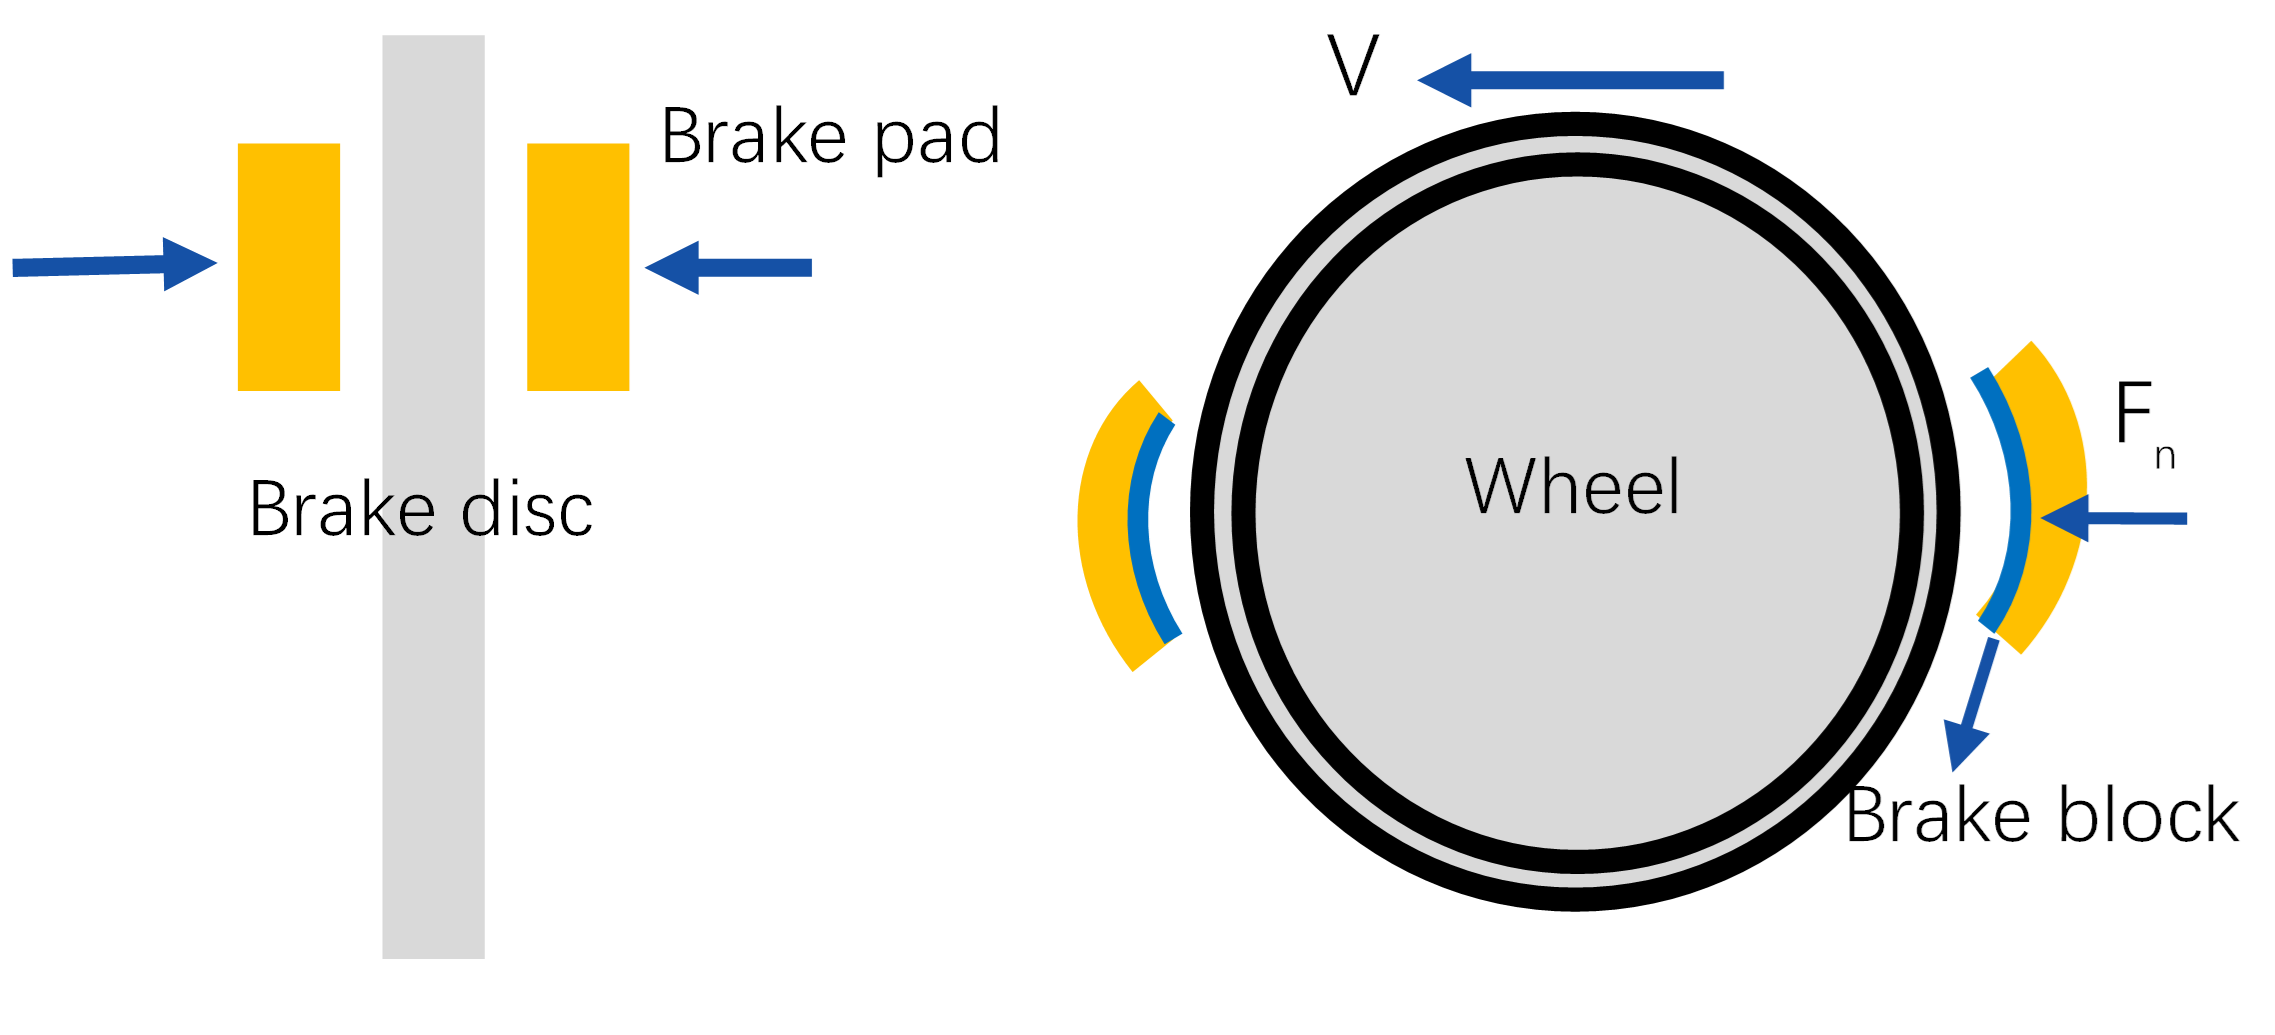
\includegraphics[width=0.65\textwidth]{book/chapters/zhang/graphics/disc_block_brakes.png}
    \caption{Block and disc brakes for rail vehicles}
    \label{fig:disc_block}
\end{figure}

Most thermal analyses of brake discs assume full contact between the brake pads and discs. From tribology studies, the real contact area is around 20\% of the whole brake pad friction surface \cite{eriksson_nature_2002}. Because of thermal expansion and wear of the brake pads, the contact area between the brake pads and discs is always changing. It is difficult to predict the true contact area. However, assuming fixed contact areas, the effect on the temperatures of brake discs can be investigated. This research aims to address the effects of different contact areas on the temperature of the brake discs.



\section*{Methods}

\subsection*{Modelling}
Heat generation and dissipation are two main parts of conducting thermal analysis of railway brake discs. Heat flux is based on friction
\begin{equation}
    q_d = \xi F_f V = \xi P A_d \mu V, 
    \label{heat flux}
\end{equation}

where \( q_d \) is the heat flux in the brake discs (W/m$^2$), \( \xi \) is the heat partition coefficient, \( F_f \) is the friction force (N), \( V \) is the velocity (m/s), \( P \) is the local contact pressure between the brake pads and discs (Pa), \( A_d \) is the friction contact area of the brake pads (m$^2$), and \( \mu \) is the coefficient of friction. Equation \ref{heat flux} is the Neumann boundary condition of Equation \ref{heat equation}, which is the overall heat transfer equation.

The heat flux distribution between the brake pads and discs is vital since it depends on how much heat flows to brake discs, which affects the temperatures and stresses. This coefficient is highly non-linear, affected by material, temperature, and pressure. In this research, this coefficient is simplified to a constant number. The distribution factor is described by \cite{rudolf_limpert_brake_1999}
\begin{equation}
    \xi = \frac{q_p}{q_d + q_p},
\end{equation}
where \( q_p \) is the heat flux in the brake pads (W/m$^2$), and \( q_d \) is the heat flux in the brake discs (W/m$^2$). 

The next step is to build a FEM model of the brake disc. FEM is a method to solve partial differential equations. This method includes the discrete domain, uses an appropriate basis, and rewrites algebraic equations. The heat equation is 
\begin{equation}
    \rho c \frac{\partial T}{\partial t} + \nabla \cdot (- k \nabla T) = f,
    \label{heat equation}
\end{equation}
where \( \rho \) is density, \( c \) is thermal capacity, \( T \) is temperature, \( t \) is time, \( k \) is the overall heat transfer coefficient, and \( f \) is the inner heat source. The time derivative on the right-hand side can be approximated by a difference quotient. Here we use the Euler backward method for consideration of numerical stability. After that, all items are multiplied by a test function \( v \) and integrated by parts. Then according to the divergence theorem, the bilinear form \( a(T,v) \) and linear form \( L(v) \) are

\begin{equation}
    a(T,v) = \frac{\rho c}{\Delta t} \int_\Omega T v dx + \int_\Omega k \nabla T \cdot \nabla v dx + \int_{\partial \Omega} h T v ds + \int_{\partial \Omega} \epsilon \sigma T^4 v ds,
\end{equation}

\begin{equation}
    L_{n+1}(v) = \int_\Omega f^{n+1} v dx 
    + \frac{\rho c}{\Delta t} \int_\Omega  T^{n} v dx 
    -  \int_{\partial \Omega} q v ds
    +  \int_{\partial \Omega} h T_a v ds 
    + \int_{\partial \Omega} \epsilon \sigma T_a^4 v ds,
\end{equation}
where \( \Omega \) is the computation domain, \( \partial \Omega \) is the boundary, \( dx \) is the differential element for integration over the domain, and \( ds \) is the differential element for integration over the boundary, \( h \) is the heat convection coefficient,  \(\Delta t\)\ is the time step, \(n\) is an integer counting time levels. The thermal radiation equation is based on Stefan-Boltzmann Law, where \( \epsilon \) is the emissivity, \( \sigma \) is Stefan-Boltzmann constant, \(T\) is the temperature and \(T^4\) is the temperature to the power of four, \( T_a \) is ambient temperature. For more detailed derivation, please see  \href{https://github.com/Yanjun96/fenicsx/blob/main/derivation_of_heat_transfer.pdf}{derivation of weak form for heat transfer equation}.

The above equation is only for heat transfer, as for brake pad deformation, one needs to solve the elastic equation and here we haven't included here. The main contribution of the elastic deformation calculation is a more accurate contact area between the brake pads and the discs. In this study, we assume that the contact area is known a priori since this research focuses on comparing the influence of different contact areas. The above equations are solved in the FEniCSx platform \cite{baratta_dolfinx_2023,scroggs_construction_2022,alnaes_unified_2014}. All the codes for this paper are in \cite{zhang_thermal_2025}.

The computation domain or mesh is shown in Figure \ref{fig:coarse mesh}. This is a much coarser mesh than the one with 1 million elements used later, with around 43,000 elements. The element type is tetrahedron since when we compared it with hexahedral elements, we found with more tetrahedron elements, the simulation can get the same accuracy with hexahedral elements while tetrahedron has less computation time. Only the brake disc and pad are computation domains. The friction heat, or the Neumann boundary condition is applied on the contact surface, more specifically, only the rubbing elements of the brake pad areas. The rubbing elements are the column structure of the brake pad. Other boundaries include radiation and convection heat transfer, which are also the Neumann boundary conditions without the heat flux input. In each time step, the boundary conditions are redefined since the rotation will change the contact area. In reality, the brake pad should keep still while the brake disc rotates. Here we assumed only the heat flux input areas are rotating: these are the friction heat input areas.

\begin{figure}[h]
    \centering
    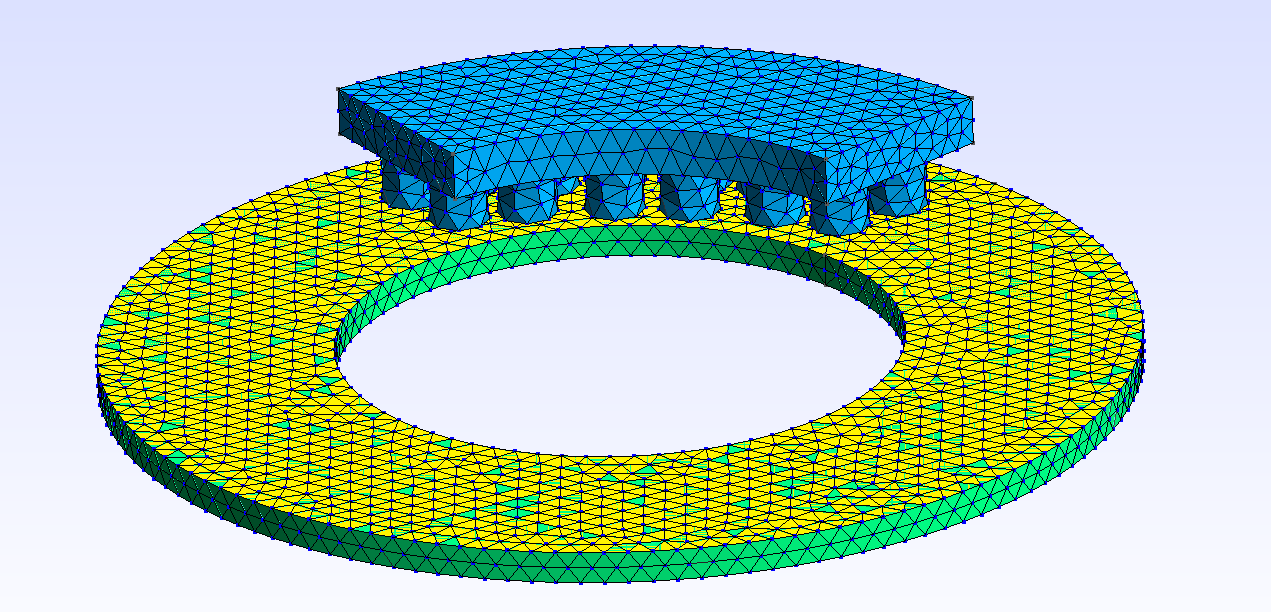
\includegraphics[width=0.9\textwidth]{book/chapters/zhang/graphics/3d surface.png}
    \caption{Computation domain of brake pad and disc, the mesh is much coarser than 1 million case. Friction heat or the Neumann boundary condition is only applied to friction contact areas.}
    \label{fig:coarse mesh}
\end{figure}


\subsection*{Experiment}

The test rig mainly consists of a DC motor, flywheels, brake pad and brake disc, as shown in Figure \ref{fig:test rig}. The maximum motor power is 450 kW, and the maximum motor torque is 4000 Nm. The brake pressure at the reservoir ranges from 0-10 Bar. 
There are in total 6 thermocouples to measure the temperature of the brake disc, which are located under the contact surface. A symmetric model is used in the simulation to save computational effort. The brake lag is the time it takes for the brake pressure to increase from 0\% to 95\% of the target pressure. In the test, the brake lag is 4±0.2 s, which follows the UIC 541-3 standard. Table \ref{tab: operational parameters} shows the operational parameters.

\begin{figure}[h]
    \centering
    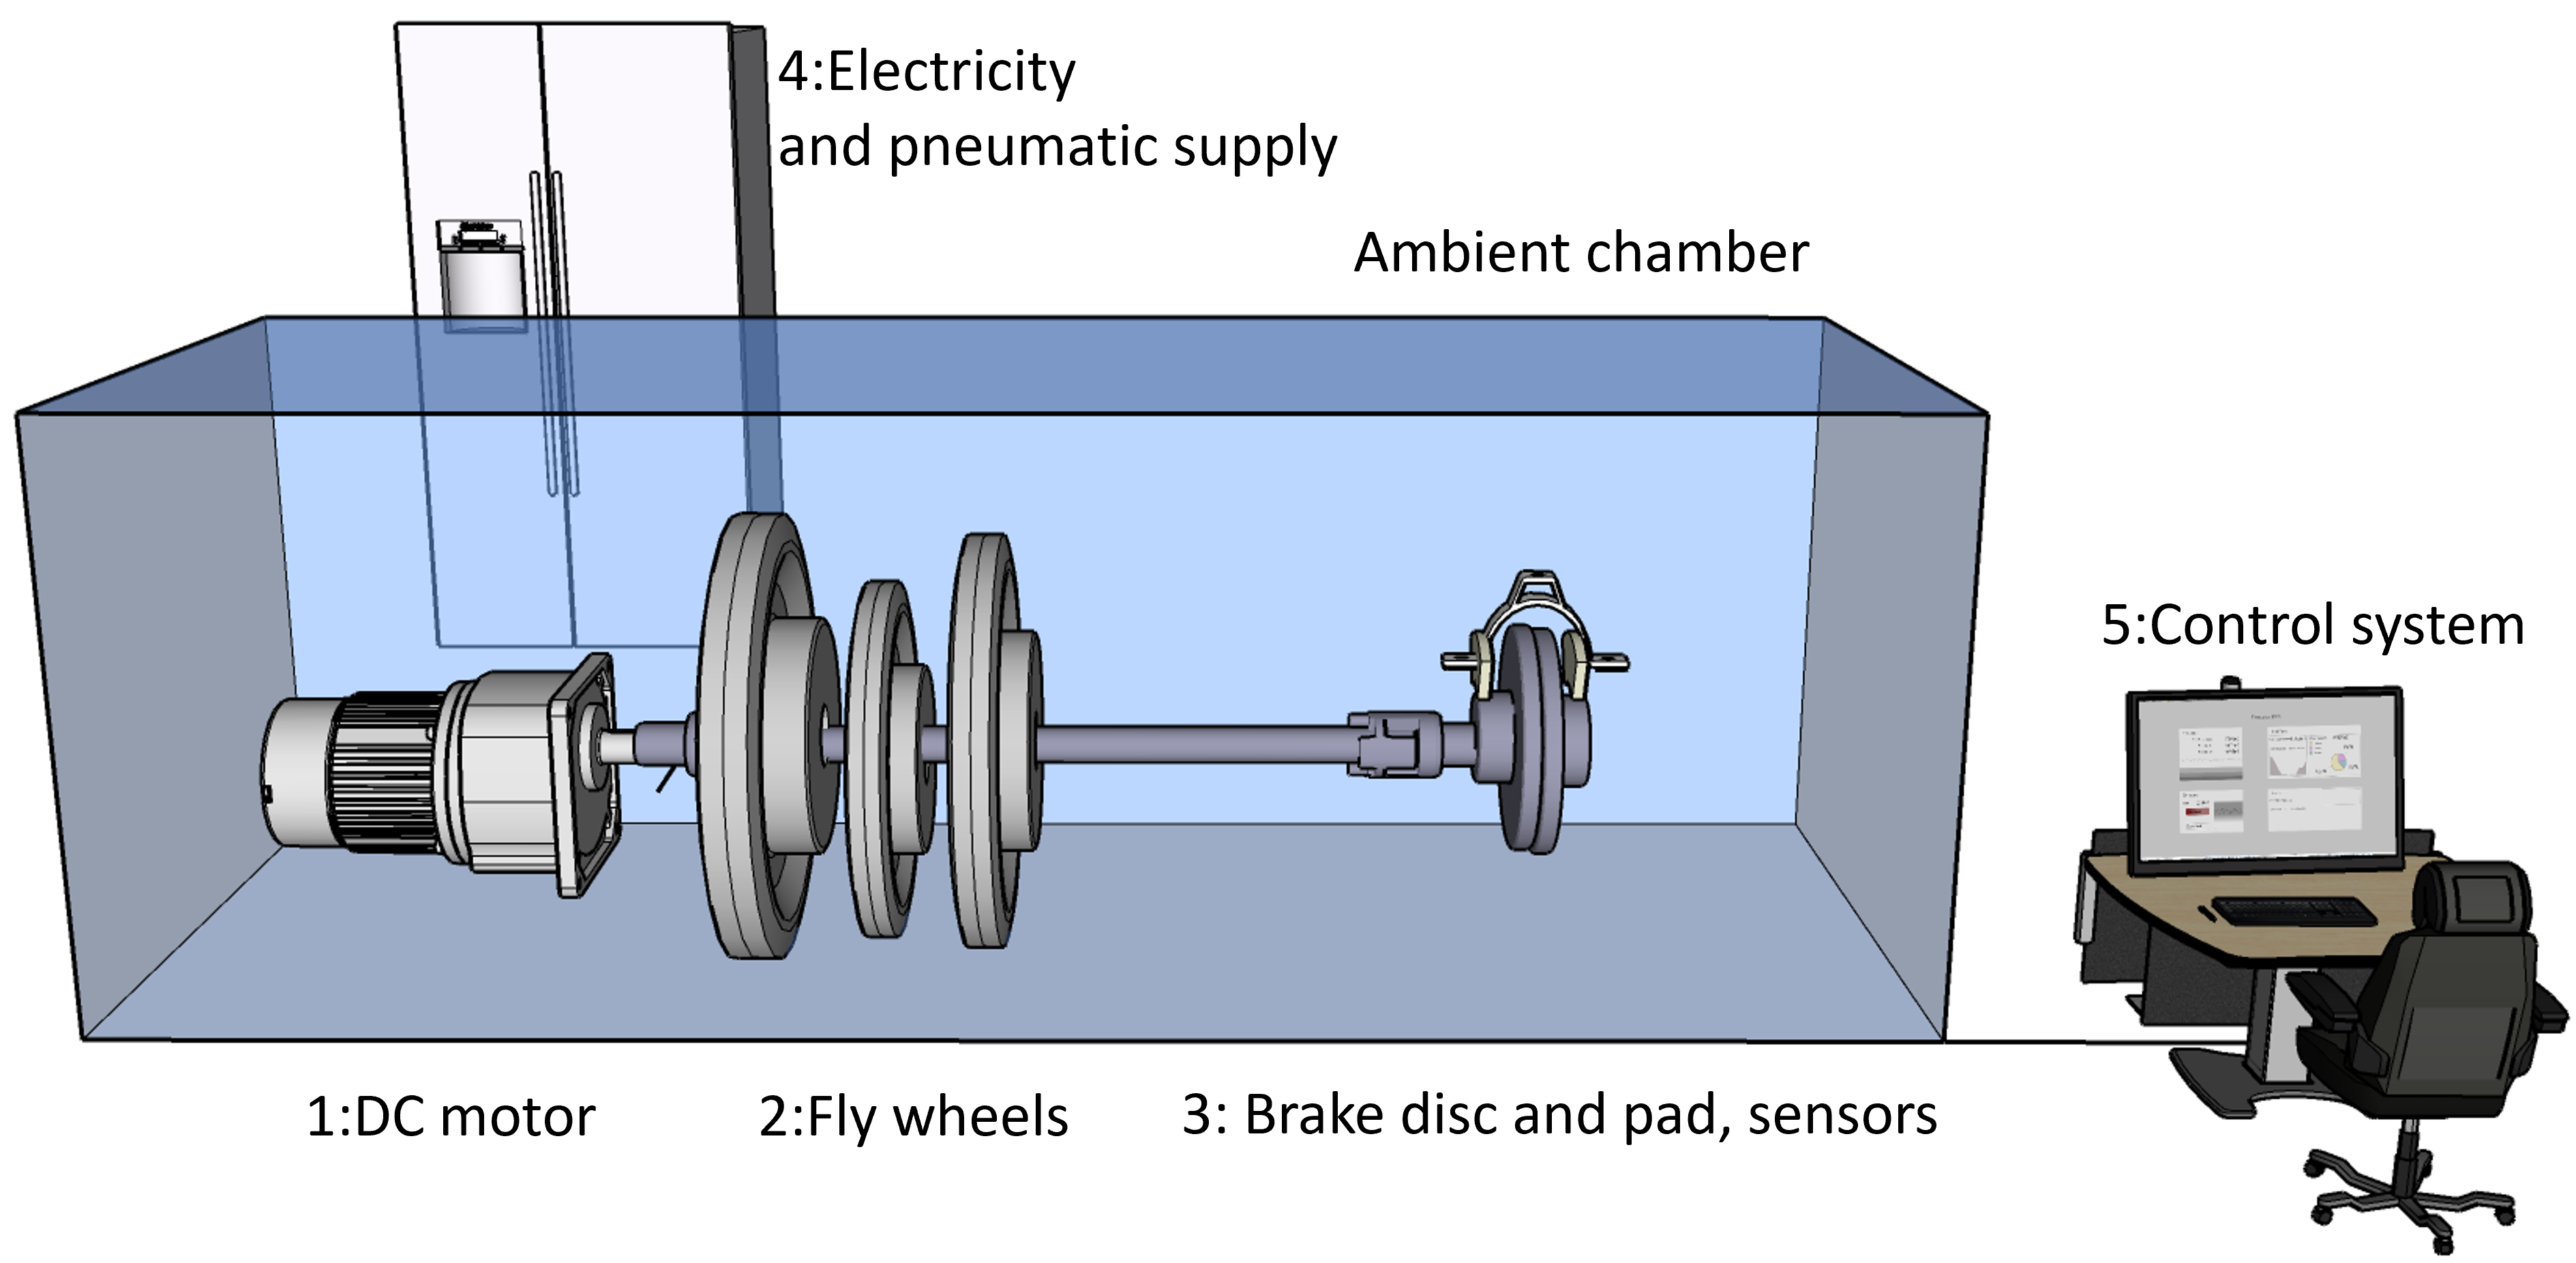
\includegraphics[width=0.85\textwidth]{book/chapters/zhang/graphics/test_rig.png}
    \caption{Full scale railway brake test rig}
    \label{fig:test rig}
\end{figure}

\begin{table}[h]
    \centering
    \begin{tabular}{llll} % 'l' for left-aligned, 'c' for centered
        \toprule
        \textbf{property} & \textbf{quantity} & \textbf{property} & \textbf{quantity}\\ % Header row
        \midrule
        initial velocity (km/h)             & 160       &braking time(s)          & 49 \\
        contact pressure (MPa)              & 0.274      &coefficient of friction  & 0.376 \\
        heat transfer coefficient( W/(m·k)) & 30-125    &heat distributor factor  & 0.88 \\
        brake lag (s)                       & 4         &initial temperature ($^\circ\text{C}$) & 50\\
       
        \bottomrule
    \end{tabular}
    \caption{Brake test parameters}
    \label{tab: operational parameters}
\end{table}

\begin{figure}[h]
    \centering
    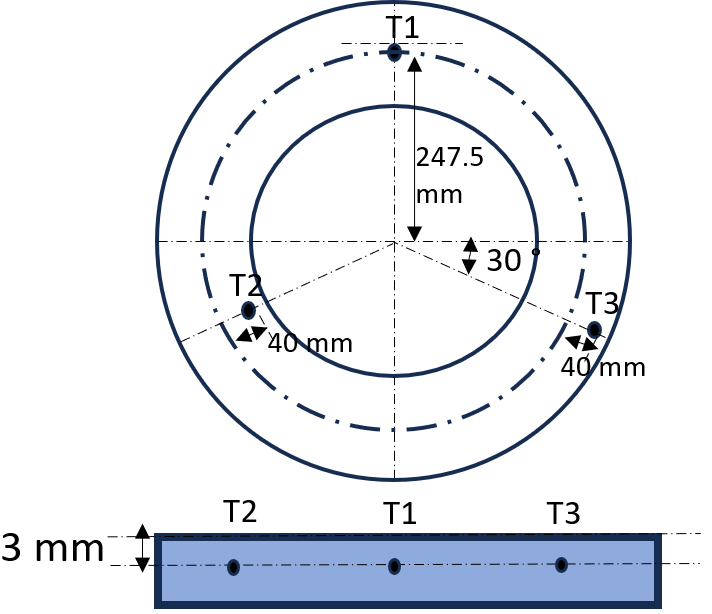
\includegraphics[width=0.45\textwidth]{book/chapters/zhang/graphics/thermo_couples.png}
    \caption{Location of three thermocouples}
    \label{fig:thermocouples}
\end{figure}


\section*{Results and discussion}

\subsection*{Validation}
The first step is mesh sensitivity and time step analysis, where we aim to show that the simulation results converge with finer mesh sizes and smaller time steps. Since no exact solution exist, the average temperature of point T1, as shown in Figure \ref{fig:thermocouples} is used as the convergence parameter.
\begin{figure}
    \centering
    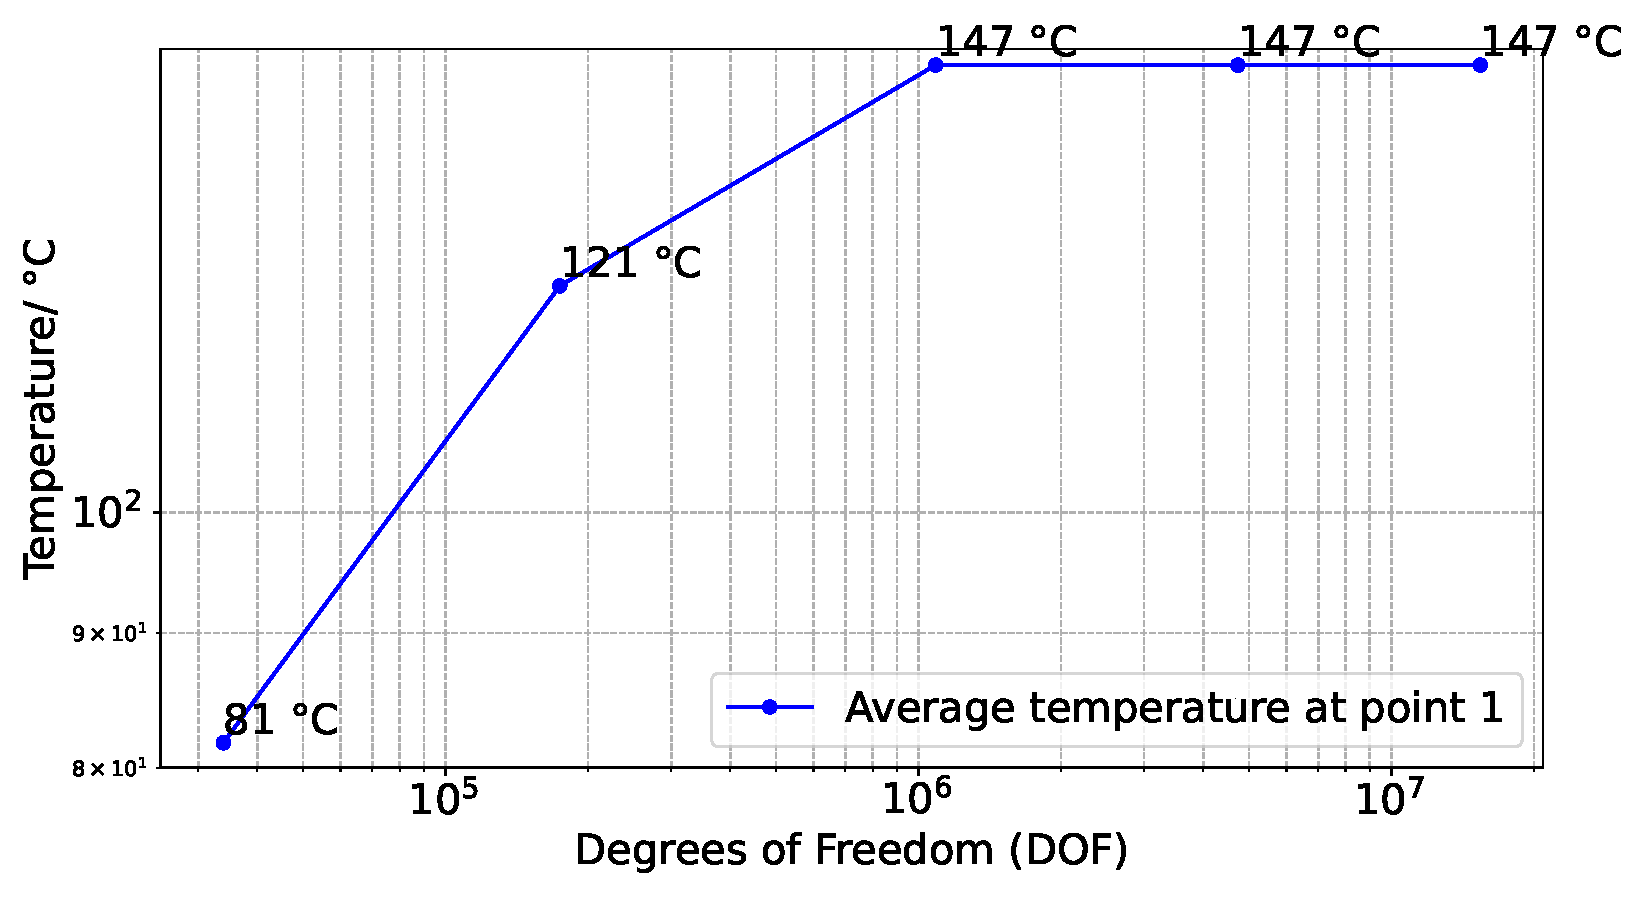
\includegraphics[width=0.8\linewidth]{book/chapters/zhang/graphics/ave_T_vs_dof.pdf}
    \caption{Convergence test, average temperatures of point T1, compared with degrees of freedom (DOFs)}
    \label{fig:error_mesh}
\end{figure}

 As shown in Figure \ref{fig:error_mesh}, the average temperature of point T1 increases with more degrees of freedom until 1 million degrees of freedom (DOFs). Above 1 million, the temperature remains constant.  The above results show that DOFs above 1 million are enough to capture the characteristics of the system. 
\begin{figure}[h]
    \centering
  
    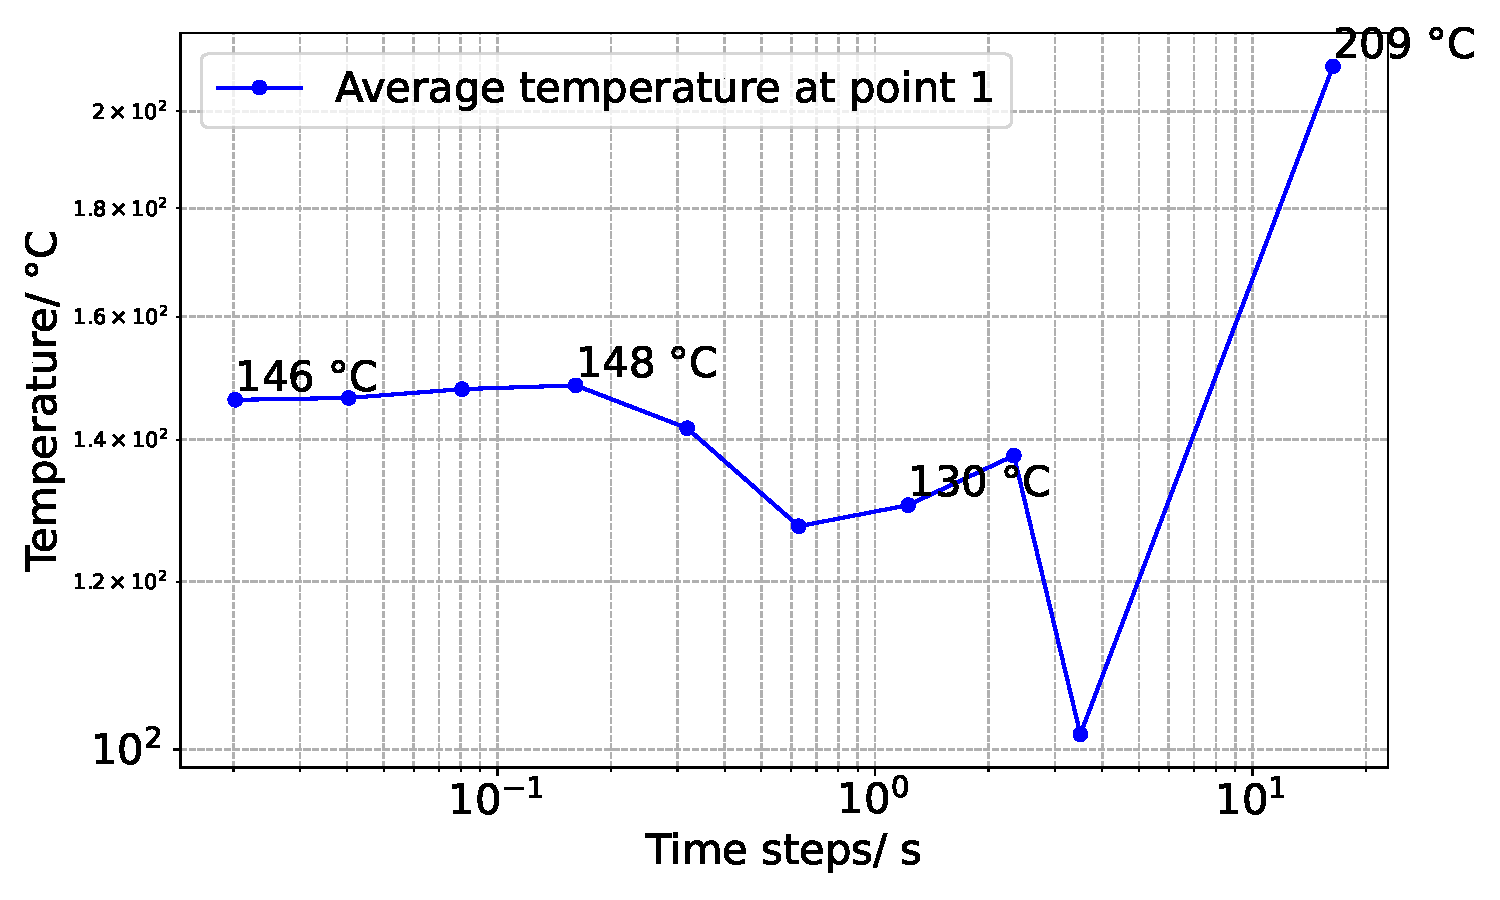
\includegraphics[width=0.8\textwidth]{book/chapters/zhang/graphics/T_ave_vs_dt.pdf}
    \caption{Convergence test, average temperatures of point T1 with time step}
    \label{fig:error_time}
\end{figure}


Figure \ref{fig:error_time} is a comparison of the average temperature of point 1 and times steps. When \(dt\) is above 1 s, the temperature has a large variance. The best value of \(dt\) is 0.16 s (point of 148$^{\circ}\text{C}$ ), which is a balance time step between accuracy and computational time.

\begin{figure}[h]
    \centering
    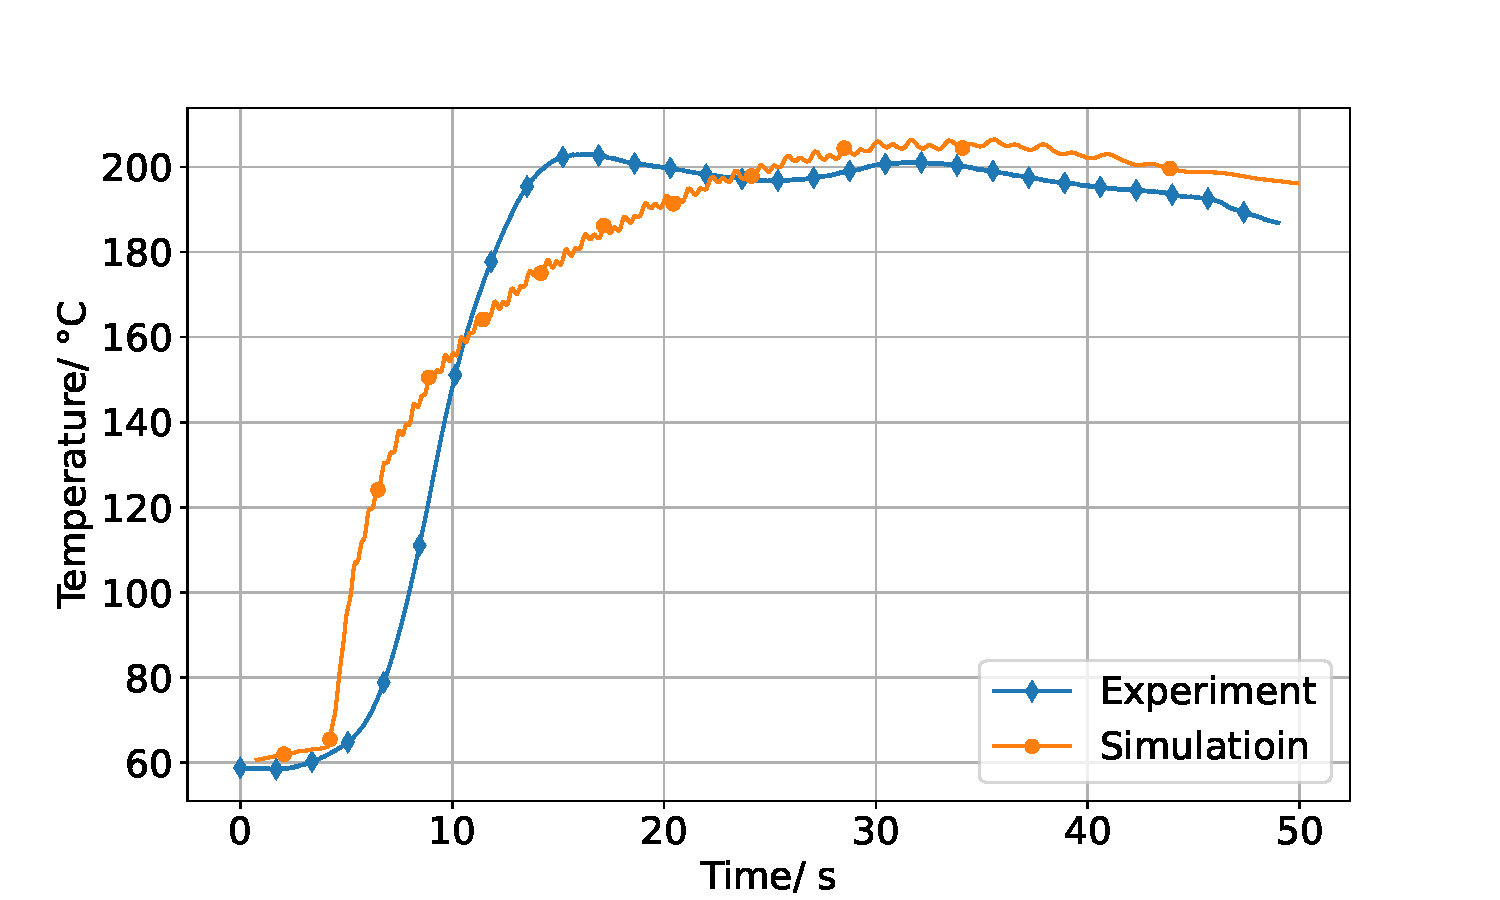
\includegraphics[width=0.8\textwidth]{book/chapters/zhang/graphics/T_sim_exe.pdf}
    \caption{Comparison between simulation time and experimental results}
    \label{fig:experiment}
\end{figure}

Except for mesh and time sensitivities analysis, the simulation results should validated against the experiment. As shown in Figure \ref{fig:experiment}. The general trend of case 1.2 million elements(4.7 million DOFs) and measurement data are the same, so we think the simulation accuracy is acceptable. However, there is still a large space to improve the accuracy. Such as introducing nonlinear material properties. These parameters, such as thermal conductivity, heat capacity, and coefficient of friction are all not constant or linear with temperature, velocity, and pressure. Getting the exact material characteristics is difficult. So better numerical results can benefit from the research of tribology and material engineering. The more detailed experiment parameters, like the loading pressure, would also significantly improve the numerical results since the experiment tests also contain large variances.



\subsection*{Average and maximum temperatures}

This section presents the temperatures of brake discs with different contact areas. The average and the maximum temperatures are presented.
The total contact surface is 200 cm$^2$. The brake pressures from the back of the brake pads are the same, 0.274 MPa, while the different contact areas will affect the contact pressure between the brake pads and discs. 20\%, 50\% and 100\% contact areas are compared. The 20\% contact areas represent the research from Eriksson \cite{eriksson_nature_2002}, and the 100\% contact areas represent most FEM or analytical solutions.

\begin{figure}[h]
    \centering
    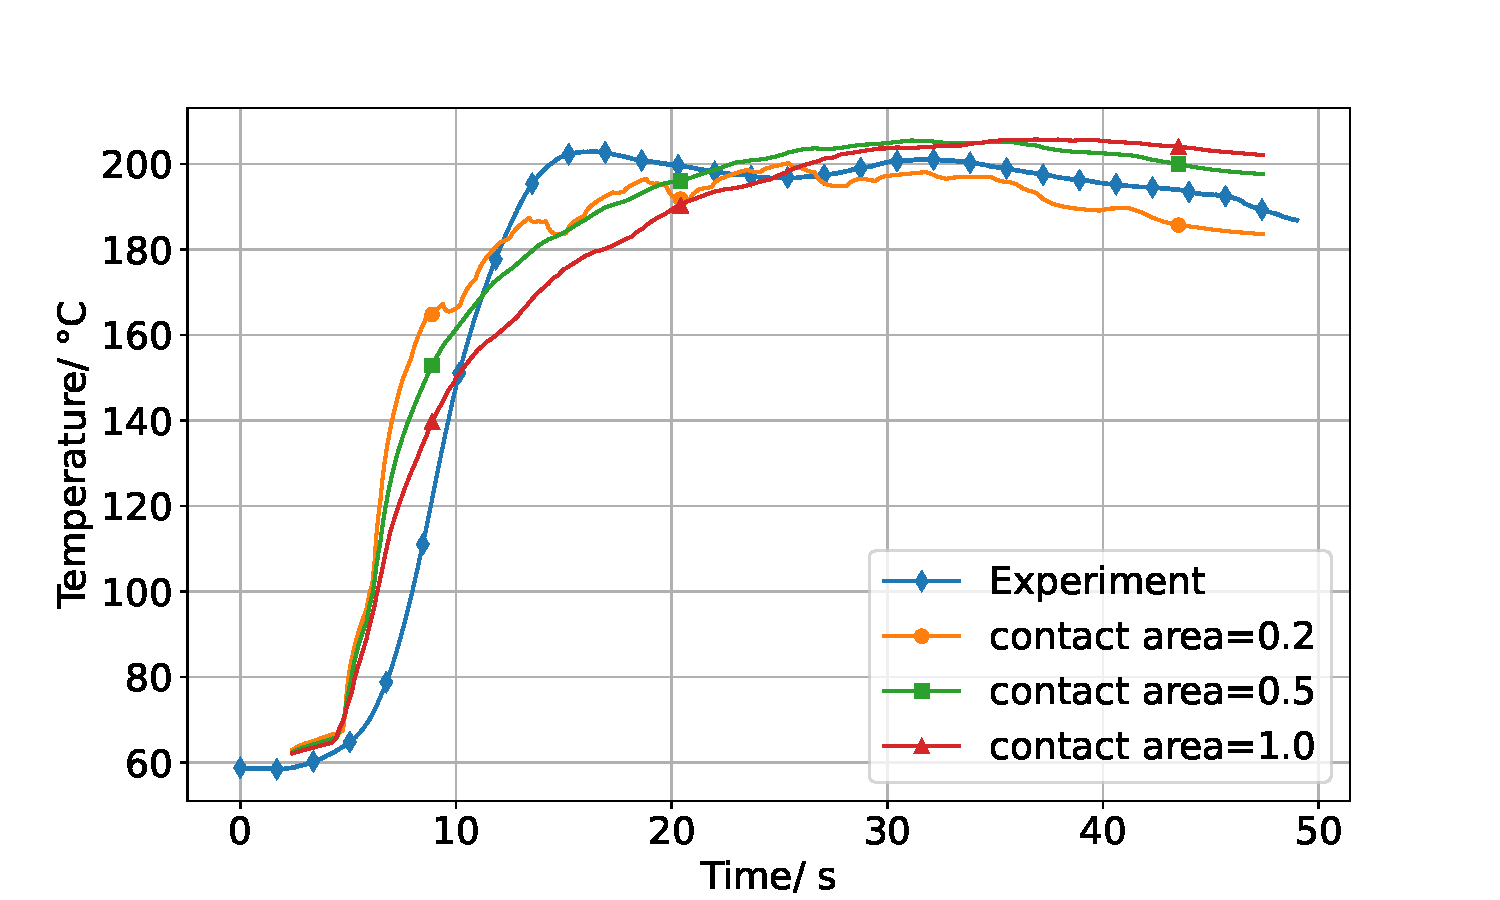
\includegraphics[width=0.8\textwidth]{book/chapters/zhang/graphics/T_ave_dc.pdf}
    \caption{Average temperatures with different contact areas}
    \label{fig:T_ave}
\end{figure}

As shown in Figure \ref{fig:T_ave} is the average temperature for these three cases. The maximum temperature difference is 20 $^{\circ}\text{C}$ between 20\% and 100\% contact areas. The maximum relative difference is 16.6\%. The average temperature is not sensitive to different contact areas since the total heat input is the same, while only heat dissipation is slightly different because the temperature distribution of the brake discs is uneven. Uneven temperature distribution can be proven through the comparison of the maximum temperatures.

\begin{figure}[h]
    \centering
    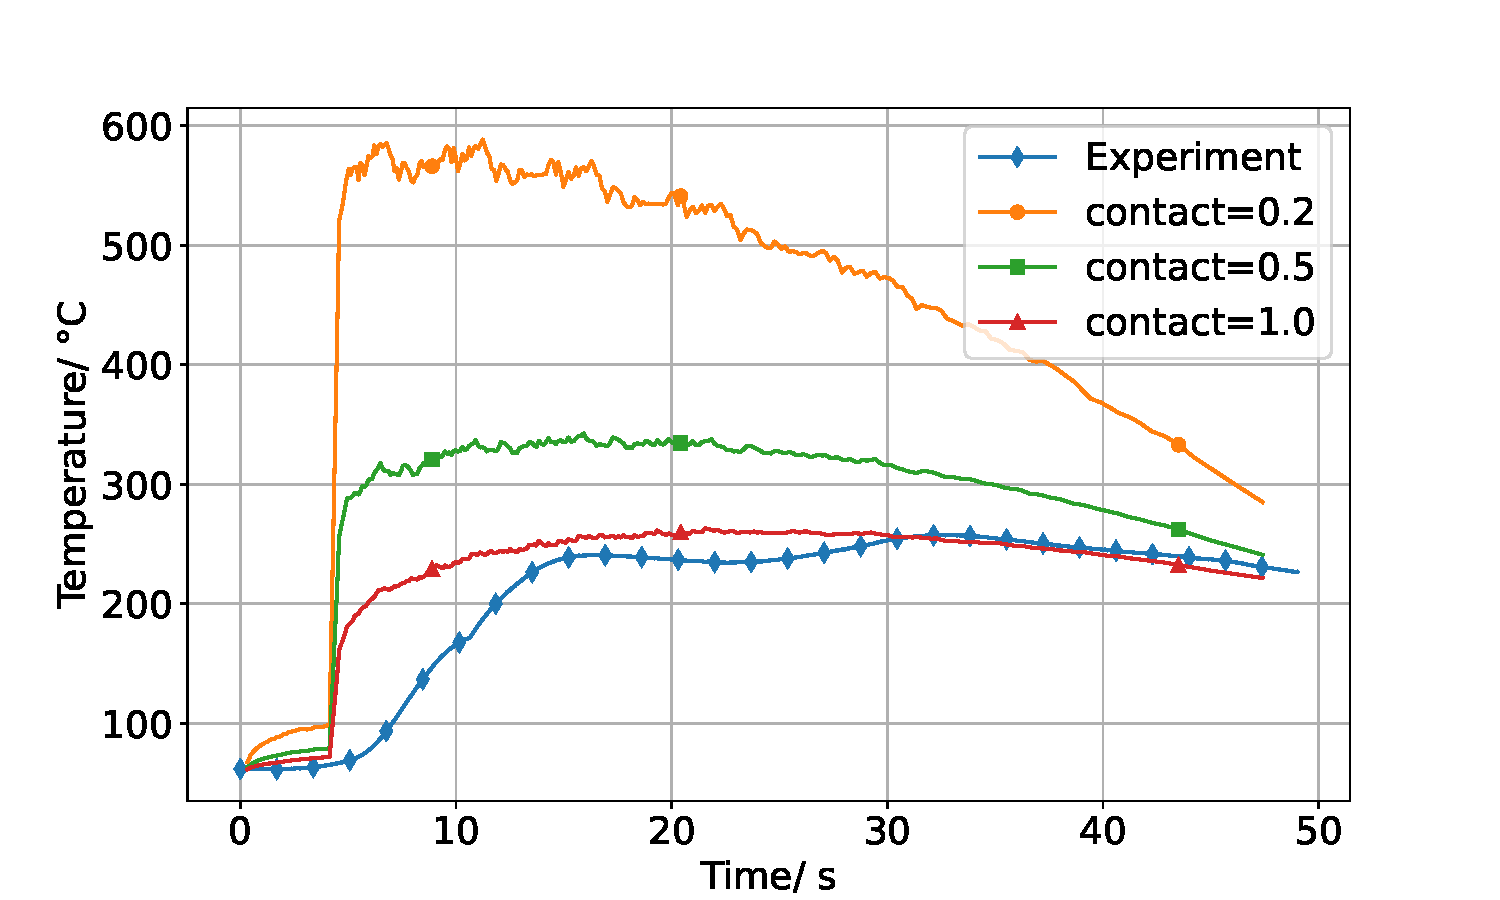
\includegraphics[width=0.8\textwidth]{book/chapters/zhang/graphics/T_max_dc.pdf}
    \caption{The maximum temperatures with different contact areas}
    \label{fig:T_max}
\end{figure}

Figure \ref{fig:T_max} shows the maximum temperature of the brake discs. The maximum temperature difference is more than 300 $^{\circ}\text{C}$, and the relative difference can reach 160\%. Small contact areas induce higher local temperatures since contact pressure is significantly increased and all friction heat is loaded on limited surfaces.

More advanced research can be conducted based on this FEM model, including sensitivity analysis of railway brake disc temperature development. In the future, the following need to be considered to build a more realistic model to investigate different brake designs:

\begin{enumerate}
\item Coupling elastic equations to get deformation details of the brake pads.
\item Considering more nonlinear parameters, like a variable coefficient of friction, and temperature-dependent material properties.
\end{enumerate}


\section*{Conclusion}
This study investigates the influence of contact area on the temperature of railway brake discs. A FEM model in FEniCSx is built and validated. The following conclusions can be drawn:
\begin{enumerate}
\item The contact area does not influence average temperature significantly while a small contact area induces a higher maximum temperature.
\item FEM based research on thermal analysis of brake systems should model real contact areas between brake pads and discs to get an accurate temperature distribution.
\end{enumerate}


\begin{acknowledgement}
This work is sponsored by the KTH Railway Group, China Scholarship Council and CRRC ZELC. Thanks to the experimental support of Fei Gao, Junying Yang at Dalian Jiaotong University. The help of Jørgen S. Dokken from the FEniCSx community and Jing Gong from Kungliga Tekniska Högskolans PDC support are especially acknowledged. Thanks to the National Academic Infrastructure for Supercomputing in Sweden for providing computer resources.        
\end{acknowledgement}

\bibliographystyle{spbasic}
% Write the full path of your bibfile relative to book.tex

\bibliography{chapters/zhang/bibliography.bib}



% Write the full path to the location of the graphics relative to book.tex
\graphicspath{{chapters/zhang/graphics/}}


\title{Thermal analysis of brake discs in rail vehicles}
\titlerunning{Thermal analysis}

\author{Yanjun Zhang, Sebastian Stichel and William Liu}
\authorrunning{Yanjun et al.}

\institute{Yanjun Zhang \email{yanjunzh@kth.se} \at KTH Royal Institute of Technology}

\maketitle

\abstract{}
Railway brake discs convert the kinetic energy of rail vehicles to thermal energy to achieve braking. This thermal energy deteriorates braking performance, therefore, it is necessary to conduct thermal analyses of brake discs. In this work, we build a FEM (finite element method) model in FEniCSx to investigate the influence of contact areas between brake pads and discs on the temperature of brake discs. The weak form of the nonlinear heat transfer equation has been derived, which accounts for conduction, convection and radiation. Multiple Neumann boundary conditions are applied. Simulation results are validated with experimental results. With this efficient FEM model, more advanced research related to railway brake discs can be conducted, such as investigating the effect of wear and thermal expansion, or designing a new geometry of the brake pads and discs.

\section*{Introduction}
Rail vehicles are developed towards higher speed and higher axle load, requiring robust mechanical brake systems for running safety. As shown in figure \ref{fig:disc_block}, one of the most important mechanical brake systems is the disc brake, which converts the kinetic energy of the rail vehicle into heat. A high brake disc temperature reduces the coefficient of friction between the brake discs and the brake pads \cite{Saffar2010}, and causes high thermal stress, which, in turn, induces thermal cracks on the brake discs. To avoid these negative impacts, it is necessary to study the temperature distribution of brake discs. Experimental investigation is relatively complex and can not obtain some parameters, while numerical study is an effective way to address this issue.

\begin{figure}[h]
    \centering
    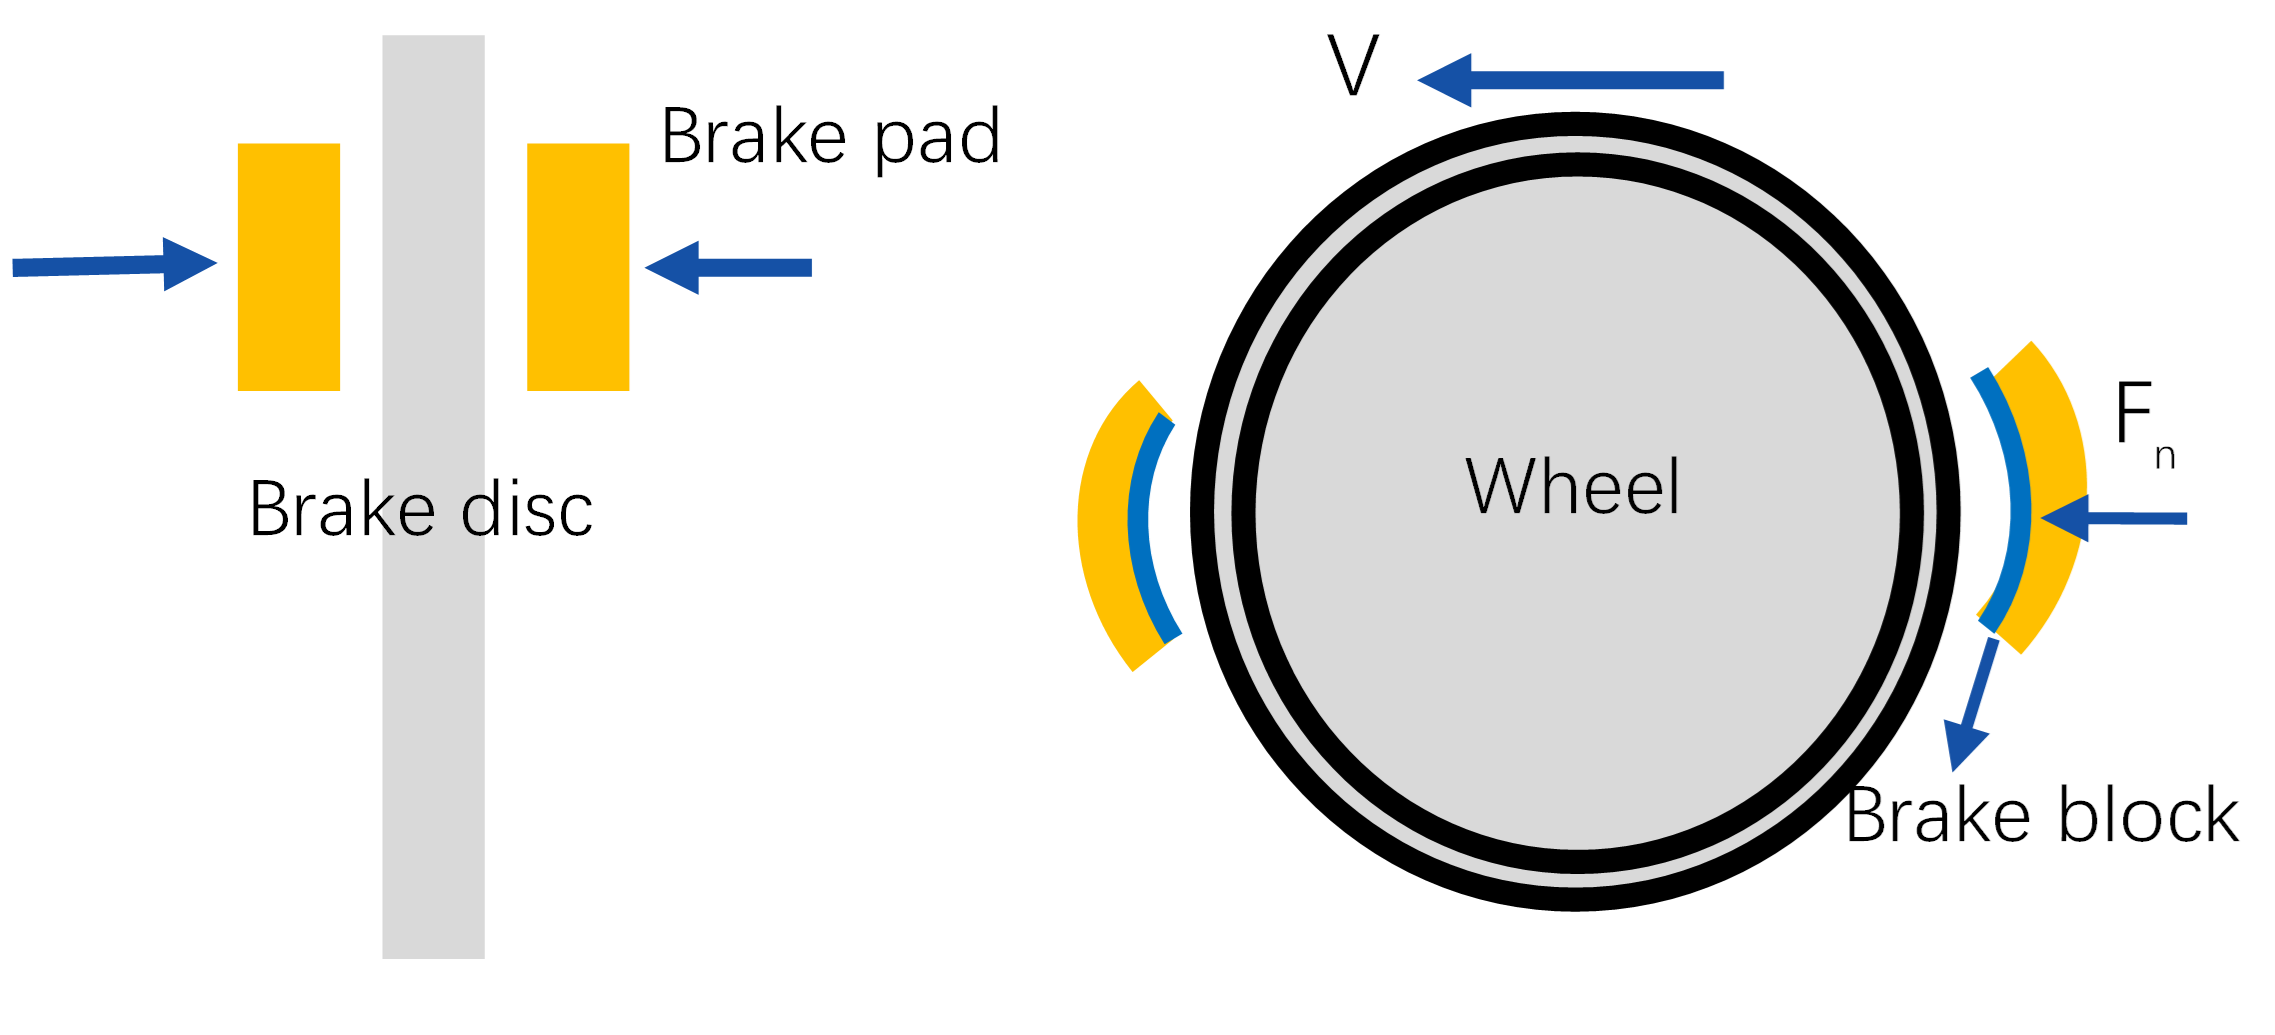
\includegraphics[width=0.65\textwidth]{book/chapters/zhang/graphics/disc_block_brakes.png}
    \caption{Block and disc brakes for rail vehicles}
    \label{fig:disc_block}
\end{figure}

Most thermal analyses of brake discs assume full contact between the brake pads and discs. From tribology studies, the real contact area is around 20\% of the whole brake pad friction surface \cite{eriksson_nature_2002}. Because of thermal expansion and wear of the brake pads, the contact area between the brake pads and discs is always changing. It is difficult to predict the true contact area. However, assuming fixed contact areas, the effect on the temperatures of brake discs can be investigated. This research aims to address the effects of different contact areas on the temperature of the brake discs.



\section*{Methods}

\subsection*{Modelling}
Heat generation and dissipation are two main parts of conducting thermal analysis of railway brake discs. Heat flux is based on friction
\begin{equation}
    q_d = \xi F_f V = \xi P A_d \mu V, 
    \label{heat flux}
\end{equation}

where \( q_d \) is the heat flux in the brake discs (W/m$^2$), \( \xi \) is the heat partition coefficient, \( F_f \) is the friction force (N), \( V \) is the velocity (m/s), \( P \) is the local contact pressure between the brake pads and discs (Pa), \( A_d \) is the friction contact area of the brake pads (m$^2$), and \( \mu \) is the coefficient of friction. Equation \ref{heat flux} is the Neumann boundary condition of Equation \ref{heat equation}, which is the overall heat transfer equation.

The heat flux distribution between the brake pads and discs is vital since it depends on how much heat flows to brake discs, which affects the temperatures and stresses. This coefficient is highly non-linear, affected by material, temperature, and pressure. In this research, this coefficient is simplified to a constant number. The distribution factor is described by \cite{rudolf_limpert_brake_1999}
\begin{equation}
    \xi = \frac{q_p}{q_d + q_p},
\end{equation}
where \( q_p \) is the heat flux in the brake pads (W/m$^2$), and \( q_d \) is the heat flux in the brake discs (W/m$^2$). 

The next step is to build a FEM model of the brake disc. FEM is a method to solve partial differential equations. This method includes the discrete domain, uses an appropriate basis, and rewrites algebraic equations. The heat equation is 
\begin{equation}
    \rho c \frac{\partial T}{\partial t} + \nabla \cdot (- k \nabla T) = f,
    \label{heat equation}
\end{equation}
where \( \rho \) is density, \( c \) is thermal capacity, \( T \) is temperature, \( t \) is time, \( k \) is the overall heat transfer coefficient, and \( f \) is the inner heat source. The time derivative on the right-hand side can be approximated by a difference quotient. Here we use the Euler backward method for consideration of numerical stability. After that, all items are multiplied by a test function \( v \) and integrated by parts. Then according to the divergence theorem, the bilinear form \( a(T,v) \) and linear form \( L(v) \) are

\begin{equation}
    a(T,v) = \frac{\rho c}{\Delta t} \int_\Omega T v dx + \int_\Omega k \nabla T \cdot \nabla v dx + \int_{\partial \Omega} h T v ds + \int_{\partial \Omega} \epsilon \sigma T^4 v ds,
\end{equation}

\begin{equation}
    L_{n+1}(v) = \int_\Omega f^{n+1} v dx 
    + \frac{\rho c}{\Delta t} \int_\Omega  T^{n} v dx 
    -  \int_{\partial \Omega} q v ds
    +  \int_{\partial \Omega} h T_a v ds 
    + \int_{\partial \Omega} \epsilon \sigma T_a^4 v ds,
\end{equation}
where \( \Omega \) is the computation domain, \( \partial \Omega \) is the boundary, \( dx \) is the differential element for integration over the domain, and \( ds \) is the differential element for integration over the boundary, \( h \) is the heat convection coefficient,  \(\Delta t\)\ is the time step, \(n\) is an integer counting time levels. The thermal radiation equation is based on Stefan-Boltzmann Law, where \( \epsilon \) is the emissivity, \( \sigma \) is Stefan-Boltzmann constant, \(T\) is the temperature and \(T^4\) is the temperature to the power of four, \( T_a \) is ambient temperature. For more detailed derivation, please see  \href{https://github.com/Yanjun96/fenicsx/blob/main/derivation_of_heat_transfer.pdf}{derivation of weak form for heat transfer equation}.

The above equation is only for heat transfer, as for brake pad deformation, one needs to solve the elastic equation and here we haven't included here. The main contribution of the elastic deformation calculation is a more accurate contact area between the brake pads and the discs. In this study, we assume that the contact area is known a priori since this research focuses on comparing the influence of different contact areas. The above equations are solved in the FEniCSx platform \cite{baratta_dolfinx_2023,scroggs_construction_2022,alnaes_unified_2014}. All the codes for this paper are in \cite{zhang_thermal_2025}.

The computation domain or mesh is shown in Figure \ref{fig:coarse mesh}. This is a much coarser mesh than the one with 1 million elements used later, with around 43,000 elements. The element type is tetrahedron since when we compared it with hexahedral elements, we found with more tetrahedron elements, the simulation can get the same accuracy with hexahedral elements while tetrahedron has less computation time. Only the brake disc and pad are computation domains. The friction heat, or the Neumann boundary condition is applied on the contact surface, more specifically, only the rubbing elements of the brake pad areas. The rubbing elements are the column structure of the brake pad. Other boundaries include radiation and convection heat transfer, which are also the Neumann boundary conditions without the heat flux input. In each time step, the boundary conditions are redefined since the rotation will change the contact area. In reality, the brake pad should keep still while the brake disc rotates. Here we assumed only the heat flux input areas are rotating: these are the friction heat input areas.

\begin{figure}[h]
    \centering
    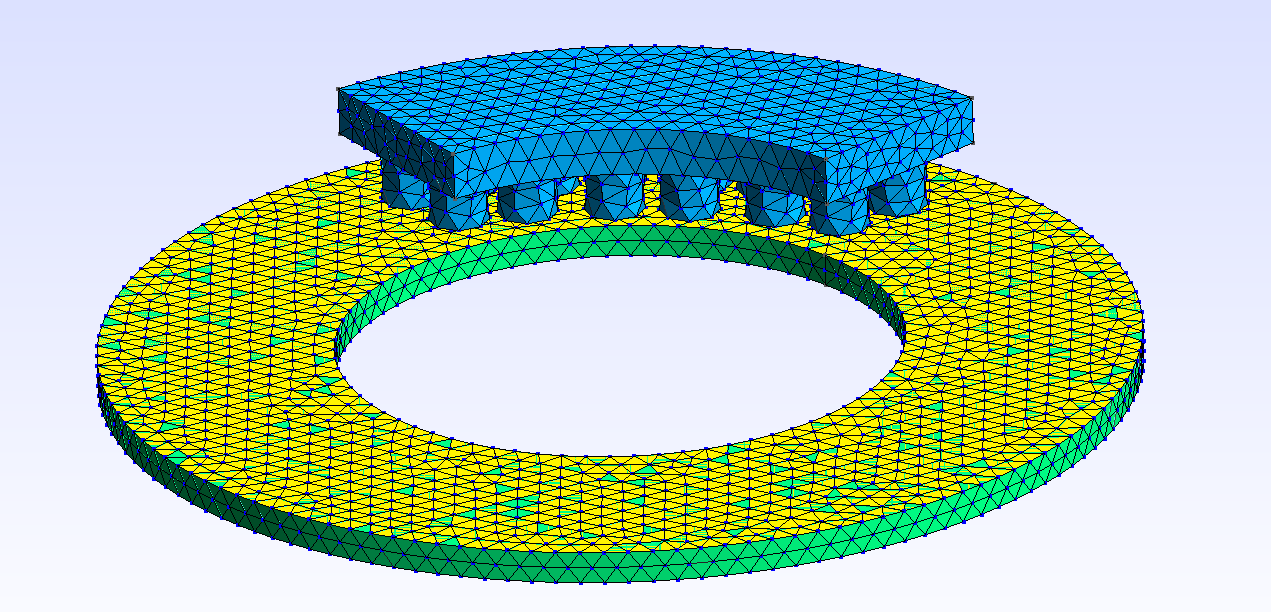
\includegraphics[width=0.9\textwidth]{book/chapters/zhang/graphics/3d surface.png}
    \caption{Computation domain of brake pad and disc, the mesh is much coarser than 1 million case. Friction heat or the Neumann boundary condition is only applied to friction contact areas.}
    \label{fig:coarse mesh}
\end{figure}


\subsection*{Experiment}

The test rig mainly consists of a DC motor, flywheels, brake pad and brake disc, as shown in Figure \ref{fig:test rig}. The maximum motor power is 450 kW, and the maximum motor torque is 4000 Nm. The brake pressure at the reservoir ranges from 0-10 Bar. 
There are in total 6 thermocouples to measure the temperature of the brake disc, which are located under the contact surface. A symmetric model is used in the simulation to save computational effort. The brake lag is the time it takes for the brake pressure to increase from 0\% to 95\% of the target pressure. In the test, the brake lag is 4±0.2 s, which follows the UIC 541-3 standard. Table \ref{tab: operational parameters} shows the operational parameters.

\begin{figure}[h]
    \centering
    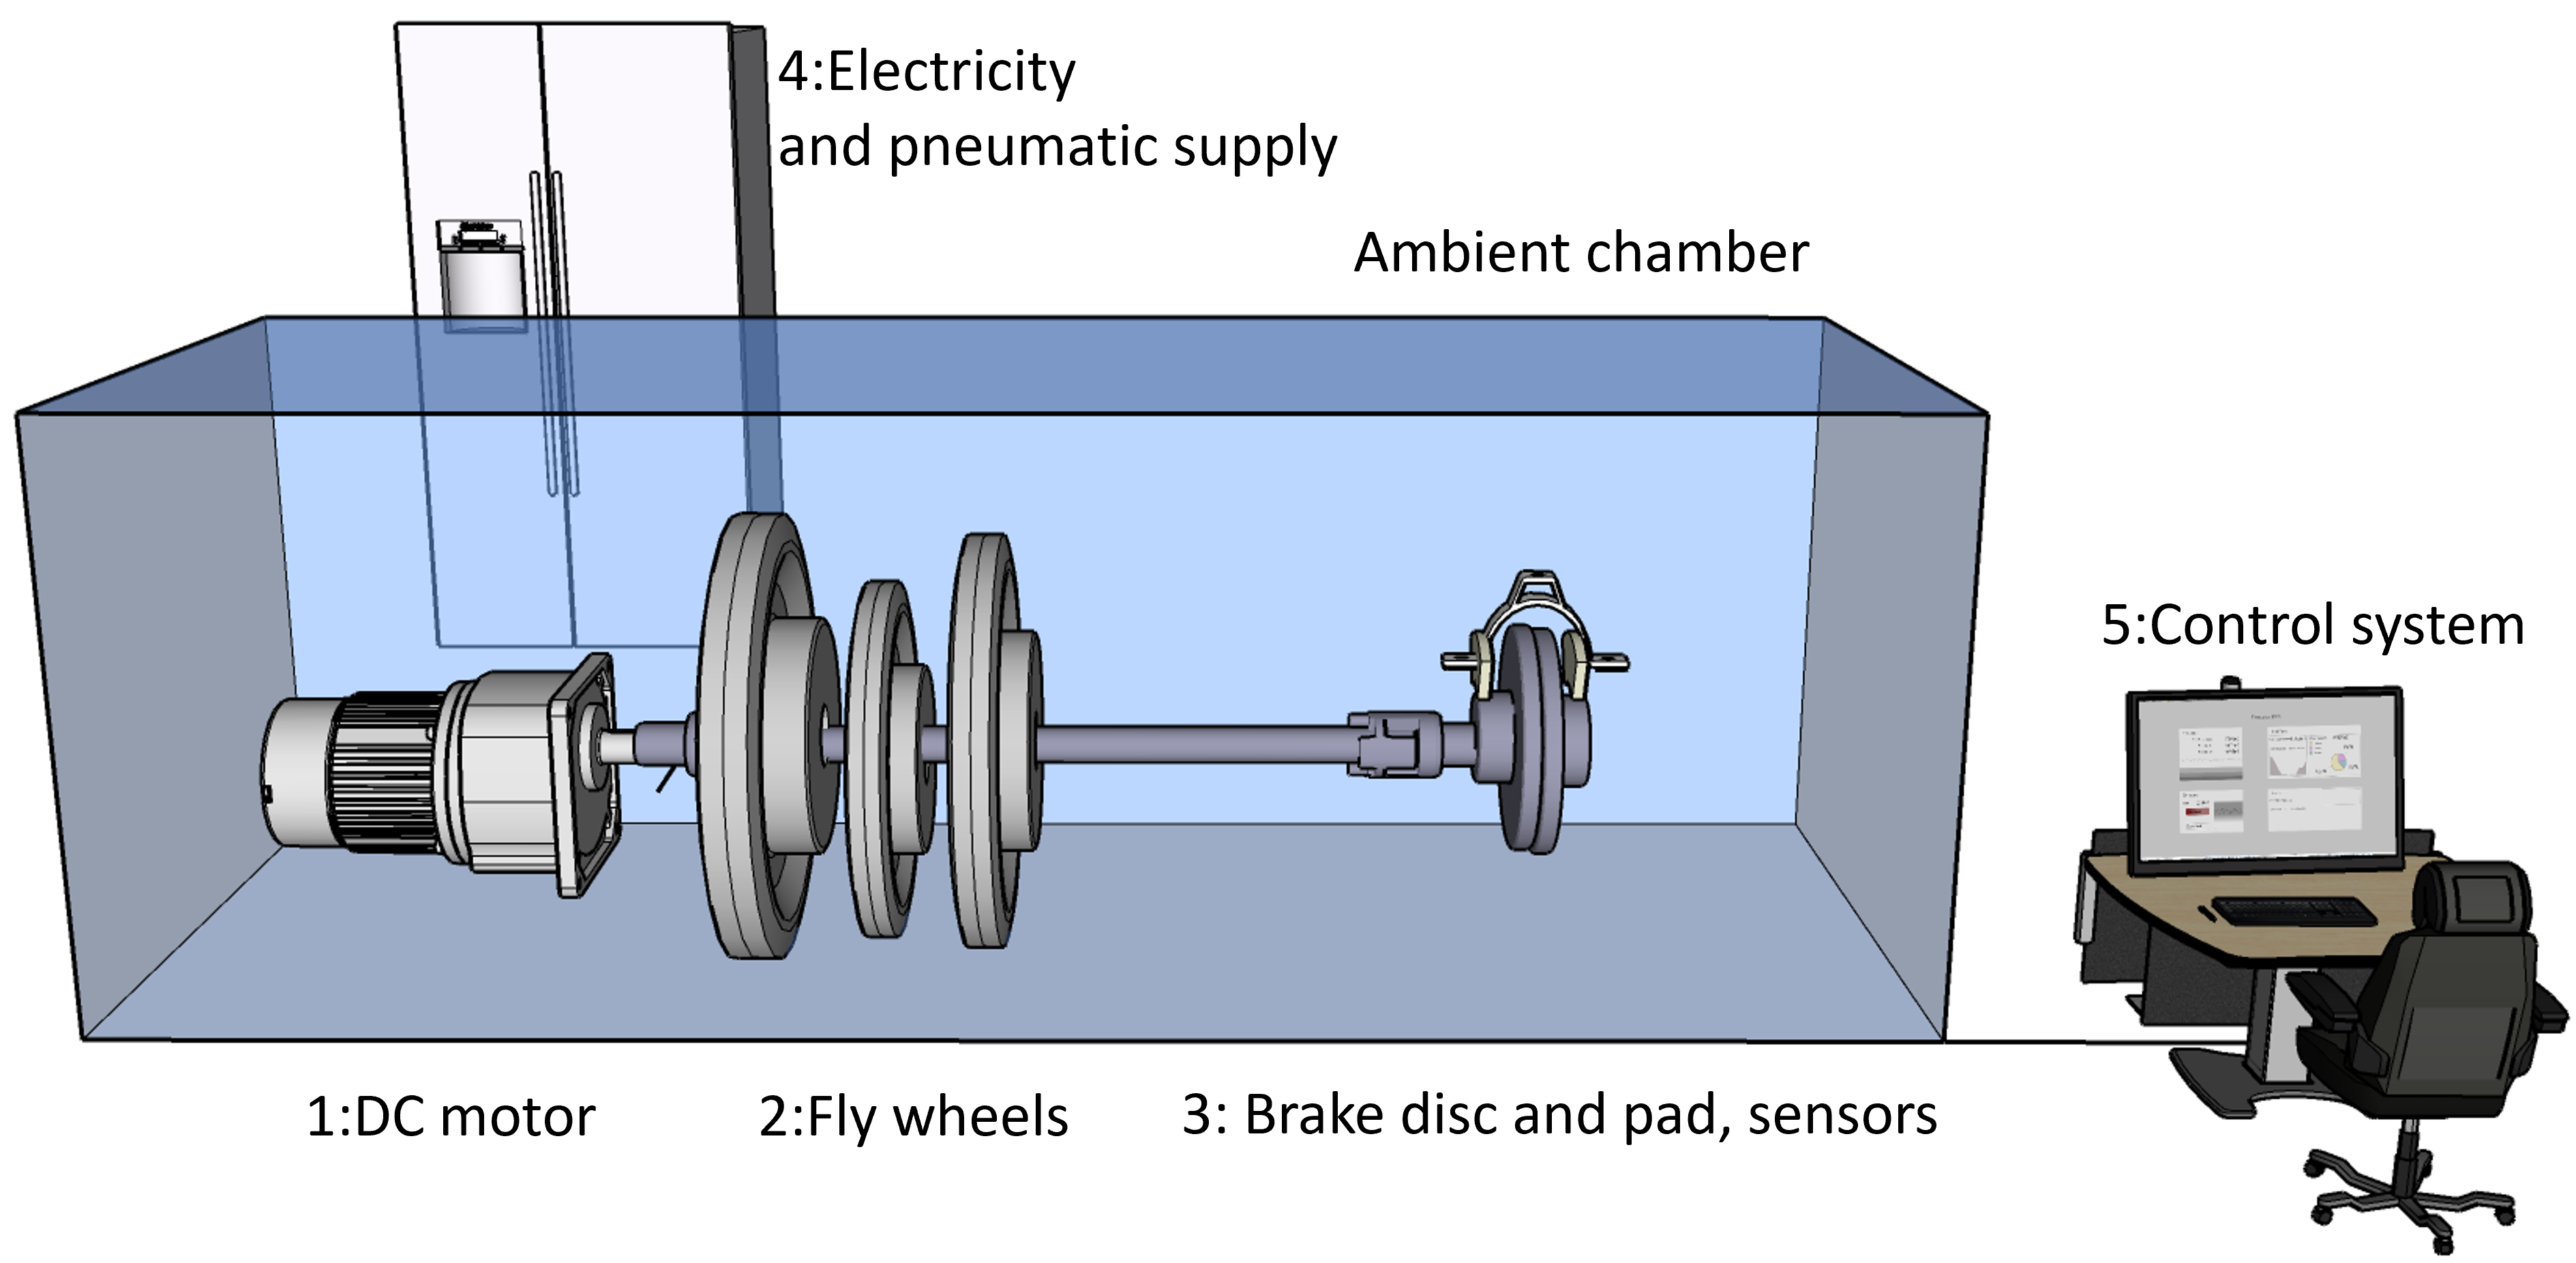
\includegraphics[width=0.85\textwidth]{book/chapters/zhang/graphics/test_rig.png}
    \caption{Full scale railway brake test rig}
    \label{fig:test rig}
\end{figure}

\begin{table}[h]
    \centering
    \begin{tabular}{llll} % 'l' for left-aligned, 'c' for centered
        \toprule
        \textbf{property} & \textbf{quantity} & \textbf{property} & \textbf{quantity}\\ % Header row
        \midrule
        initial velocity (km/h)             & 160       &braking time(s)          & 49 \\
        contact pressure (MPa)              & 0.274      &coefficient of friction  & 0.376 \\
        heat transfer coefficient( W/(m·k)) & 30-125    &heat distributor factor  & 0.88 \\
        brake lag (s)                       & 4         &initial temperature ($^\circ\text{C}$) & 50\\
       
        \bottomrule
    \end{tabular}
    \caption{Brake test parameters}
    \label{tab: operational parameters}
\end{table}

\begin{figure}[h]
    \centering
    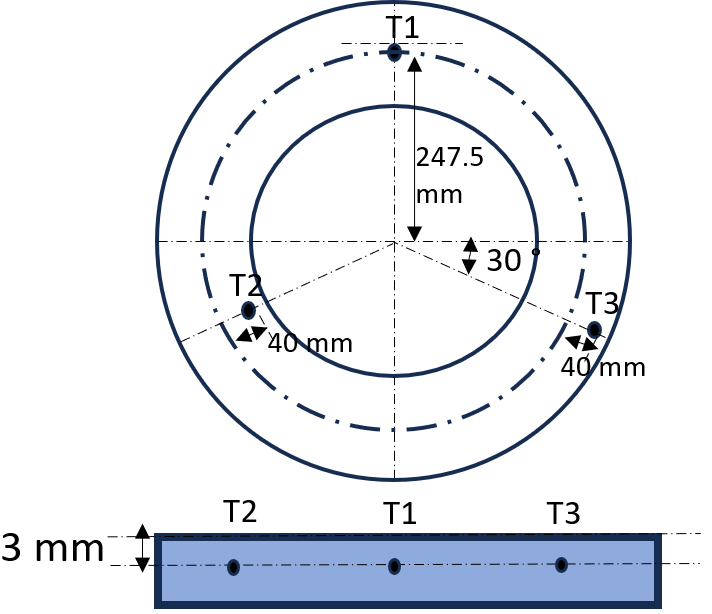
\includegraphics[width=0.45\textwidth]{book/chapters/zhang/graphics/thermo_couples.png}
    \caption{Location of three thermocouples}
    \label{fig:thermocouples}
\end{figure}


\section*{Results and discussion}

\subsection*{Validation}
The first step is mesh sensitivity and time step analysis, where we aim to show that the simulation results converge with finer mesh sizes and smaller time steps. Since no exact solution exist, the average temperature of point T1, as shown in Figure \ref{fig:thermocouples} is used as the convergence parameter.
\begin{figure}
    \centering
    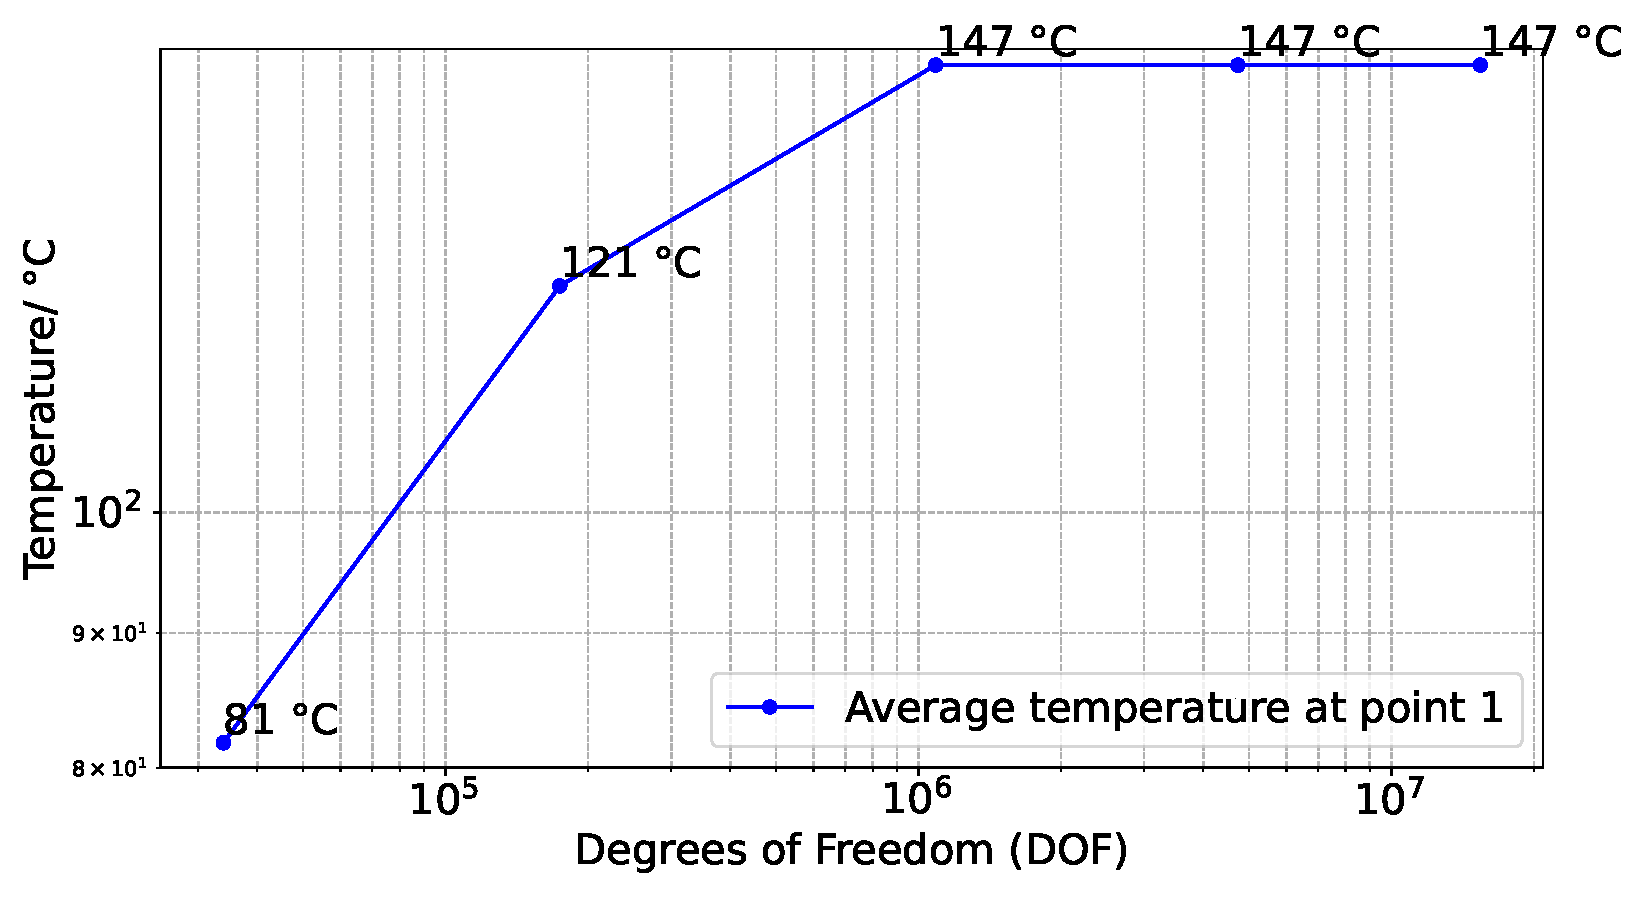
\includegraphics[width=0.8\linewidth]{book/chapters/zhang/graphics/ave_T_vs_dof.pdf}
    \caption{Convergence test, average temperatures of point T1, compared with degrees of freedom (DOFs)}
    \label{fig:error_mesh}
\end{figure}

 As shown in Figure \ref{fig:error_mesh}, the average temperature of point T1 increases with more degrees of freedom until 1 million degrees of freedom (DOFs). Above 1 million, the temperature remains constant.  The above results show that DOFs above 1 million are enough to capture the characteristics of the system. 
\begin{figure}[h]
    \centering
  
    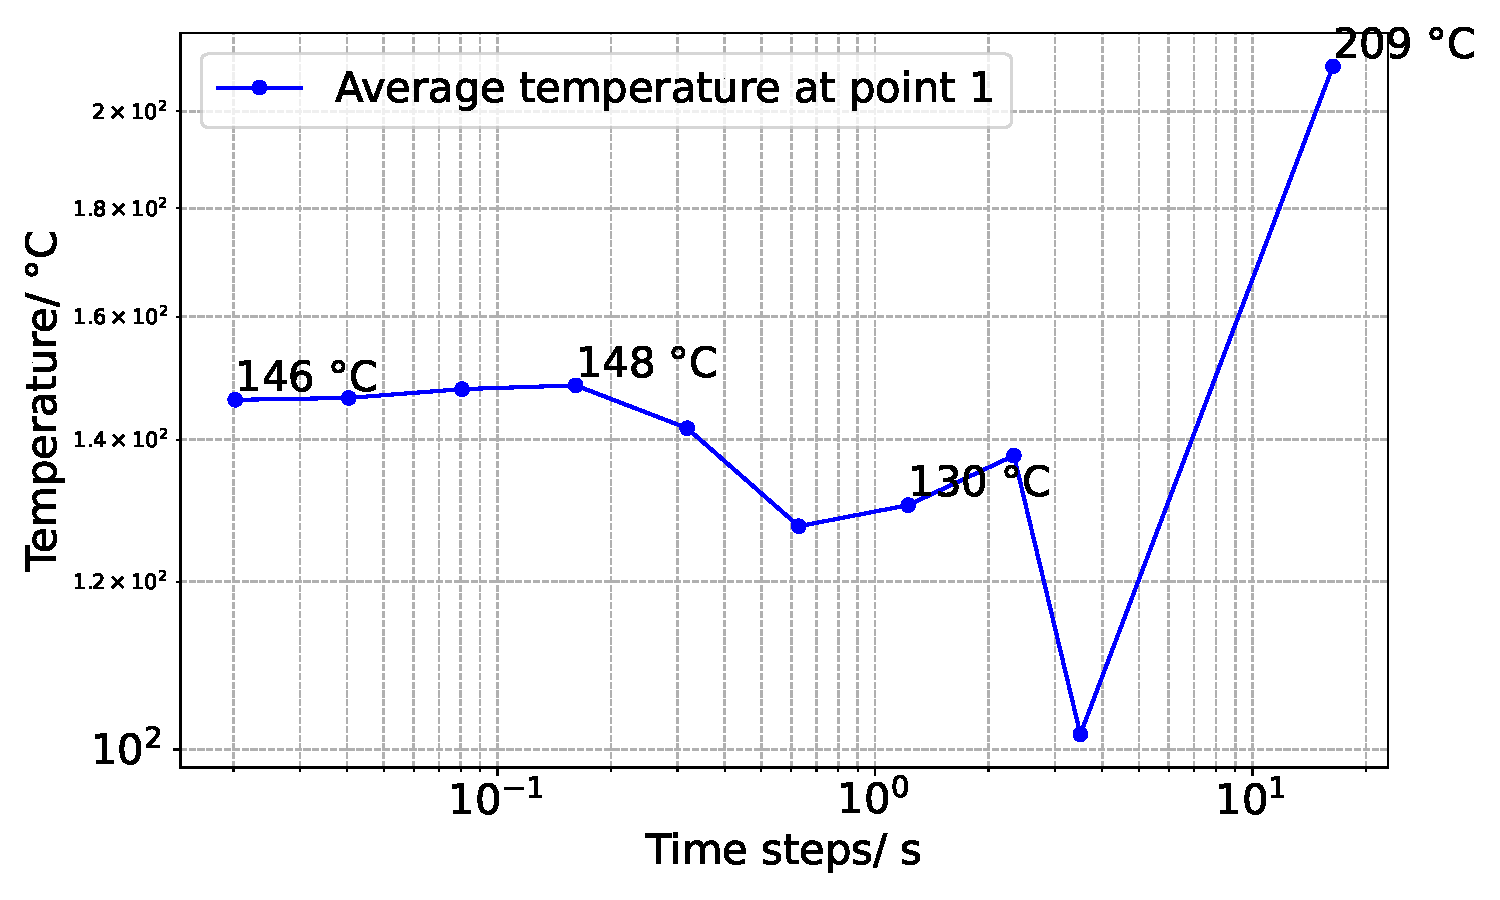
\includegraphics[width=0.8\textwidth]{book/chapters/zhang/graphics/T_ave_vs_dt.pdf}
    \caption{Convergence test, average temperatures of point T1 with time step}
    \label{fig:error_time}
\end{figure}


Figure \ref{fig:error_time} is a comparison of the average temperature of point 1 and times steps. When \(dt\) is above 1 s, the temperature has a large variance. The best value of \(dt\) is 0.16 s (point of 148$^{\circ}\text{C}$ ), which is a balance time step between accuracy and computational time.

\begin{figure}[h]
    \centering
    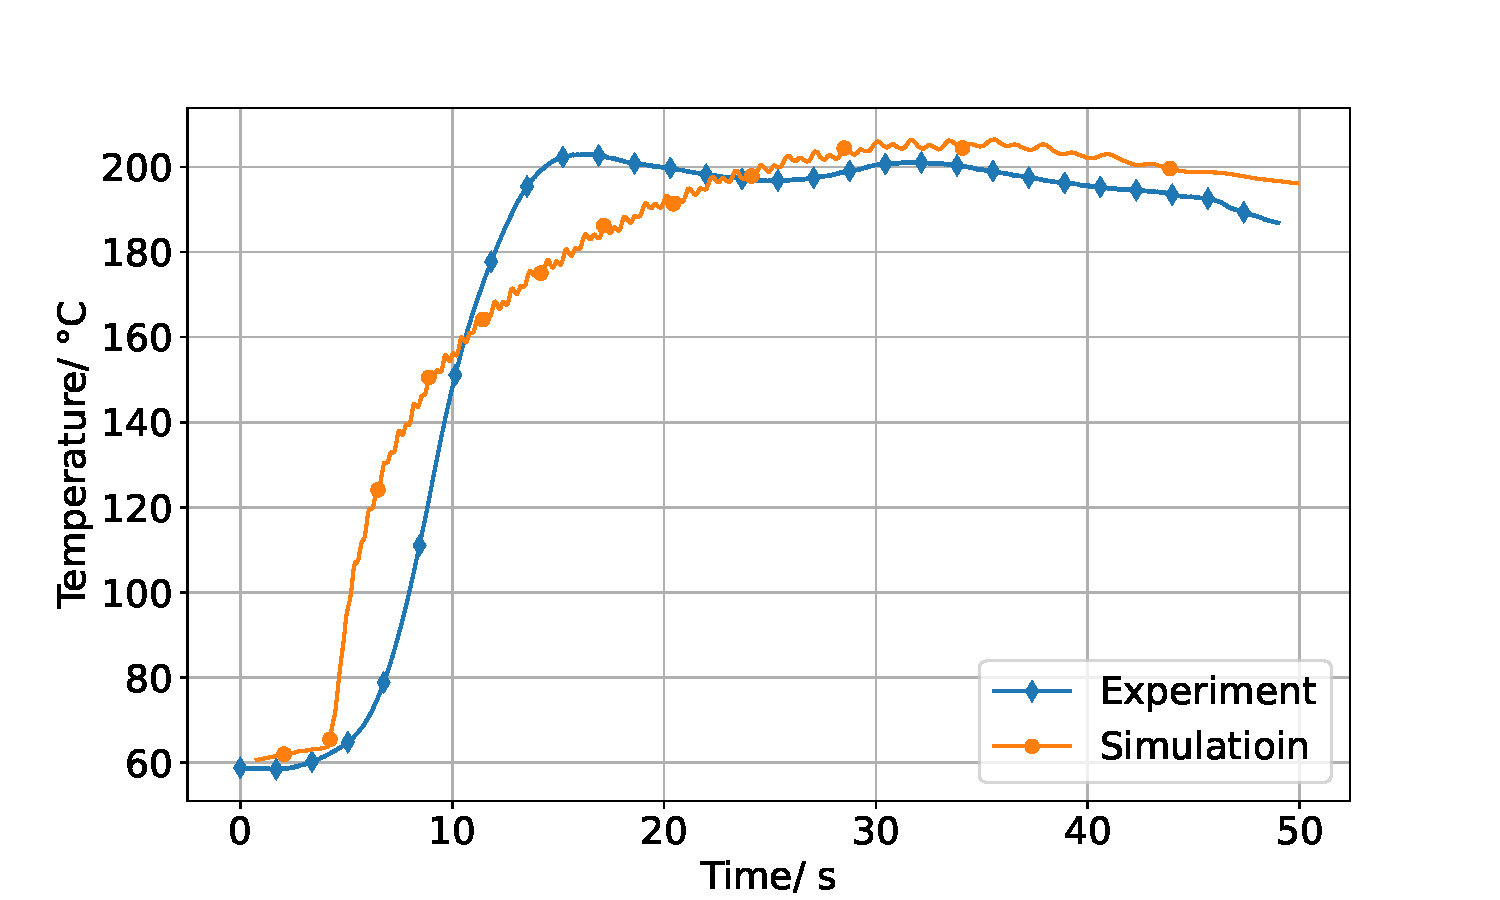
\includegraphics[width=0.8\textwidth]{book/chapters/zhang/graphics/T_sim_exe.pdf}
    \caption{Comparison between simulation time and experimental results}
    \label{fig:experiment}
\end{figure}

Except for mesh and time sensitivities analysis, the simulation results should validated against the experiment. As shown in Figure \ref{fig:experiment}. The general trend of case 1.2 million elements(4.7 million DOFs) and measurement data are the same, so we think the simulation accuracy is acceptable. However, there is still a large space to improve the accuracy. Such as introducing nonlinear material properties. These parameters, such as thermal conductivity, heat capacity, and coefficient of friction are all not constant or linear with temperature, velocity, and pressure. Getting the exact material characteristics is difficult. So better numerical results can benefit from the research of tribology and material engineering. The more detailed experiment parameters, like the loading pressure, would also significantly improve the numerical results since the experiment tests also contain large variances.



\subsection*{Average and maximum temperatures}

This section presents the temperatures of brake discs with different contact areas. The average and the maximum temperatures are presented.
The total contact surface is 200 cm$^2$. The brake pressures from the back of the brake pads are the same, 0.274 MPa, while the different contact areas will affect the contact pressure between the brake pads and discs. 20\%, 50\% and 100\% contact areas are compared. The 20\% contact areas represent the research from Eriksson \cite{eriksson_nature_2002}, and the 100\% contact areas represent most FEM or analytical solutions.

\begin{figure}[h]
    \centering
    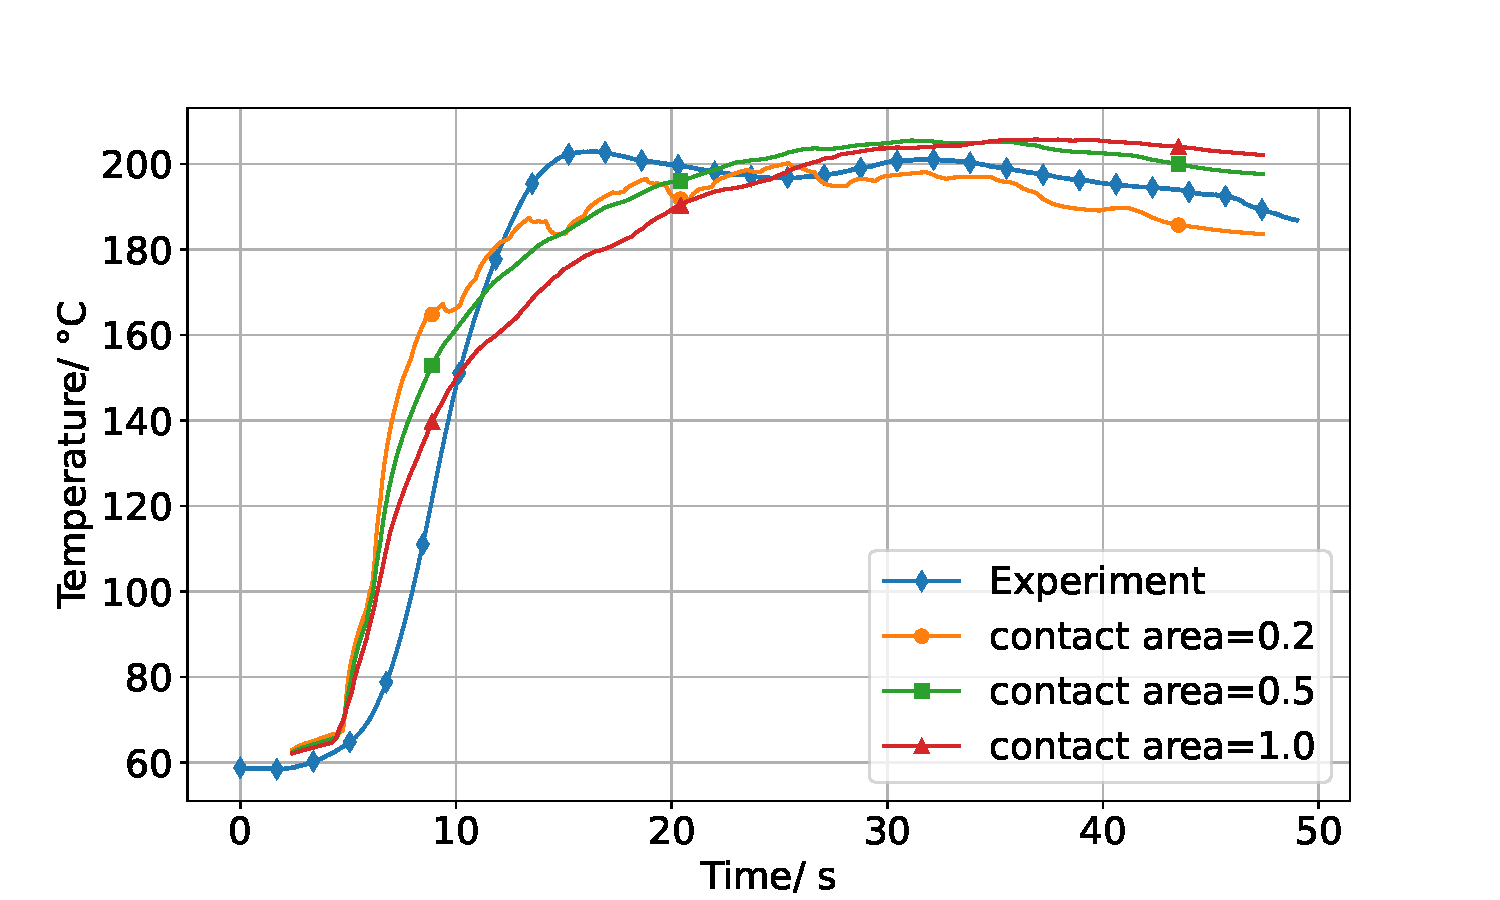
\includegraphics[width=0.8\textwidth]{book/chapters/zhang/graphics/T_ave_dc.pdf}
    \caption{Average temperatures with different contact areas}
    \label{fig:T_ave}
\end{figure}

As shown in Figure \ref{fig:T_ave} is the average temperature for these three cases. The maximum temperature difference is 20 $^{\circ}\text{C}$ between 20\% and 100\% contact areas. The maximum relative difference is 16.6\%. The average temperature is not sensitive to different contact areas since the total heat input is the same, while only heat dissipation is slightly different because the temperature distribution of the brake discs is uneven. Uneven temperature distribution can be proven through the comparison of the maximum temperatures.

\begin{figure}[h]
    \centering
    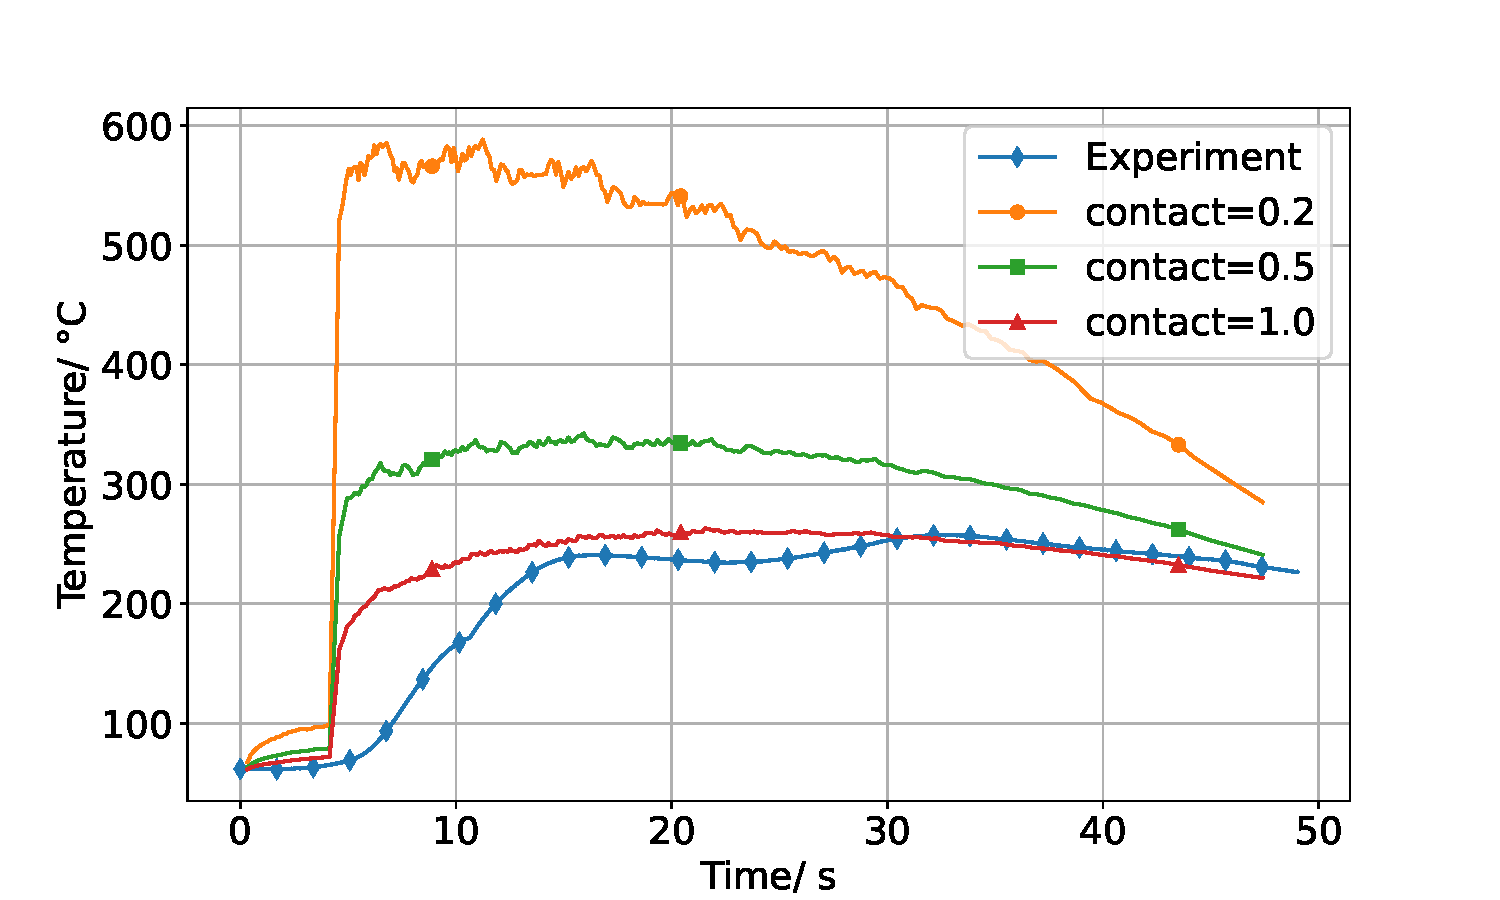
\includegraphics[width=0.8\textwidth]{book/chapters/zhang/graphics/T_max_dc.pdf}
    \caption{The maximum temperatures with different contact areas}
    \label{fig:T_max}
\end{figure}

Figure \ref{fig:T_max} shows the maximum temperature of the brake discs. The maximum temperature difference is more than 300 $^{\circ}\text{C}$, and the relative difference can reach 160\%. Small contact areas induce higher local temperatures since contact pressure is significantly increased and all friction heat is loaded on limited surfaces.

More advanced research can be conducted based on this FEM model, including sensitivity analysis of railway brake disc temperature development. In the future, the following need to be considered to build a more realistic model to investigate different brake designs:

\begin{enumerate}
\item Coupling elastic equations to get deformation details of the brake pads.
\item Considering more nonlinear parameters, like a variable coefficient of friction, and temperature-dependent material properties.
\end{enumerate}


\section*{Conclusion}
This study investigates the influence of contact area on the temperature of railway brake discs. A FEM model in FEniCSx is built and validated. The following conclusions can be drawn:
\begin{enumerate}
\item The contact area does not influence average temperature significantly while a small contact area induces a higher maximum temperature.
\item FEM based research on thermal analysis of brake systems should model real contact areas between brake pads and discs to get an accurate temperature distribution.
\end{enumerate}


\begin{acknowledgement}
This work is sponsored by the KTH Railway Group, China Scholarship Council and CRRC ZELC. Thanks to the experimental support of Fei Gao, Junying Yang at Dalian Jiaotong University. The help of Jørgen S. Dokken from the FEniCSx community and Jing Gong from Kungliga Tekniska Högskolans PDC support are especially acknowledged. Thanks to the National Academic Infrastructure for Supercomputing in Sweden for providing computer resources.        
\end{acknowledgement}

\bibliographystyle{spbasic}
% Write the full path of your bibfile relative to book.tex

\bibliography{chapters/zhang/bibliography.bib}


 
% Write the full path to the location of the graphics relative to book.tex
\graphicspath{{chapters/zhang/graphics/}}


\title{Thermal analysis of brake discs in rail vehicles}
\titlerunning{Thermal analysis}

\author{Yanjun Zhang, Sebastian Stichel and William Liu}
\authorrunning{Yanjun et al.}

\institute{Yanjun Zhang \email{yanjunzh@kth.se} \at KTH Royal Institute of Technology}

\maketitle

\abstract{}
Railway brake discs convert the kinetic energy of rail vehicles to thermal energy to achieve braking. This thermal energy deteriorates braking performance, therefore, it is necessary to conduct thermal analyses of brake discs. In this work, we build a FEM (finite element method) model in FEniCSx to investigate the influence of contact areas between brake pads and discs on the temperature of brake discs. The weak form of the nonlinear heat transfer equation has been derived, which accounts for conduction, convection and radiation. Multiple Neumann boundary conditions are applied. Simulation results are validated with experimental results. With this efficient FEM model, more advanced research related to railway brake discs can be conducted, such as investigating the effect of wear and thermal expansion, or designing a new geometry of the brake pads and discs.

\section*{Introduction}
Rail vehicles are developed towards higher speed and higher axle load, requiring robust mechanical brake systems for running safety. As shown in figure \ref{fig:disc_block}, one of the most important mechanical brake systems is the disc brake, which converts the kinetic energy of the rail vehicle into heat. A high brake disc temperature reduces the coefficient of friction between the brake discs and the brake pads \cite{Saffar2010}, and causes high thermal stress, which, in turn, induces thermal cracks on the brake discs. To avoid these negative impacts, it is necessary to study the temperature distribution of brake discs. Experimental investigation is relatively complex and can not obtain some parameters, while numerical study is an effective way to address this issue.

\begin{figure}[h]
    \centering
    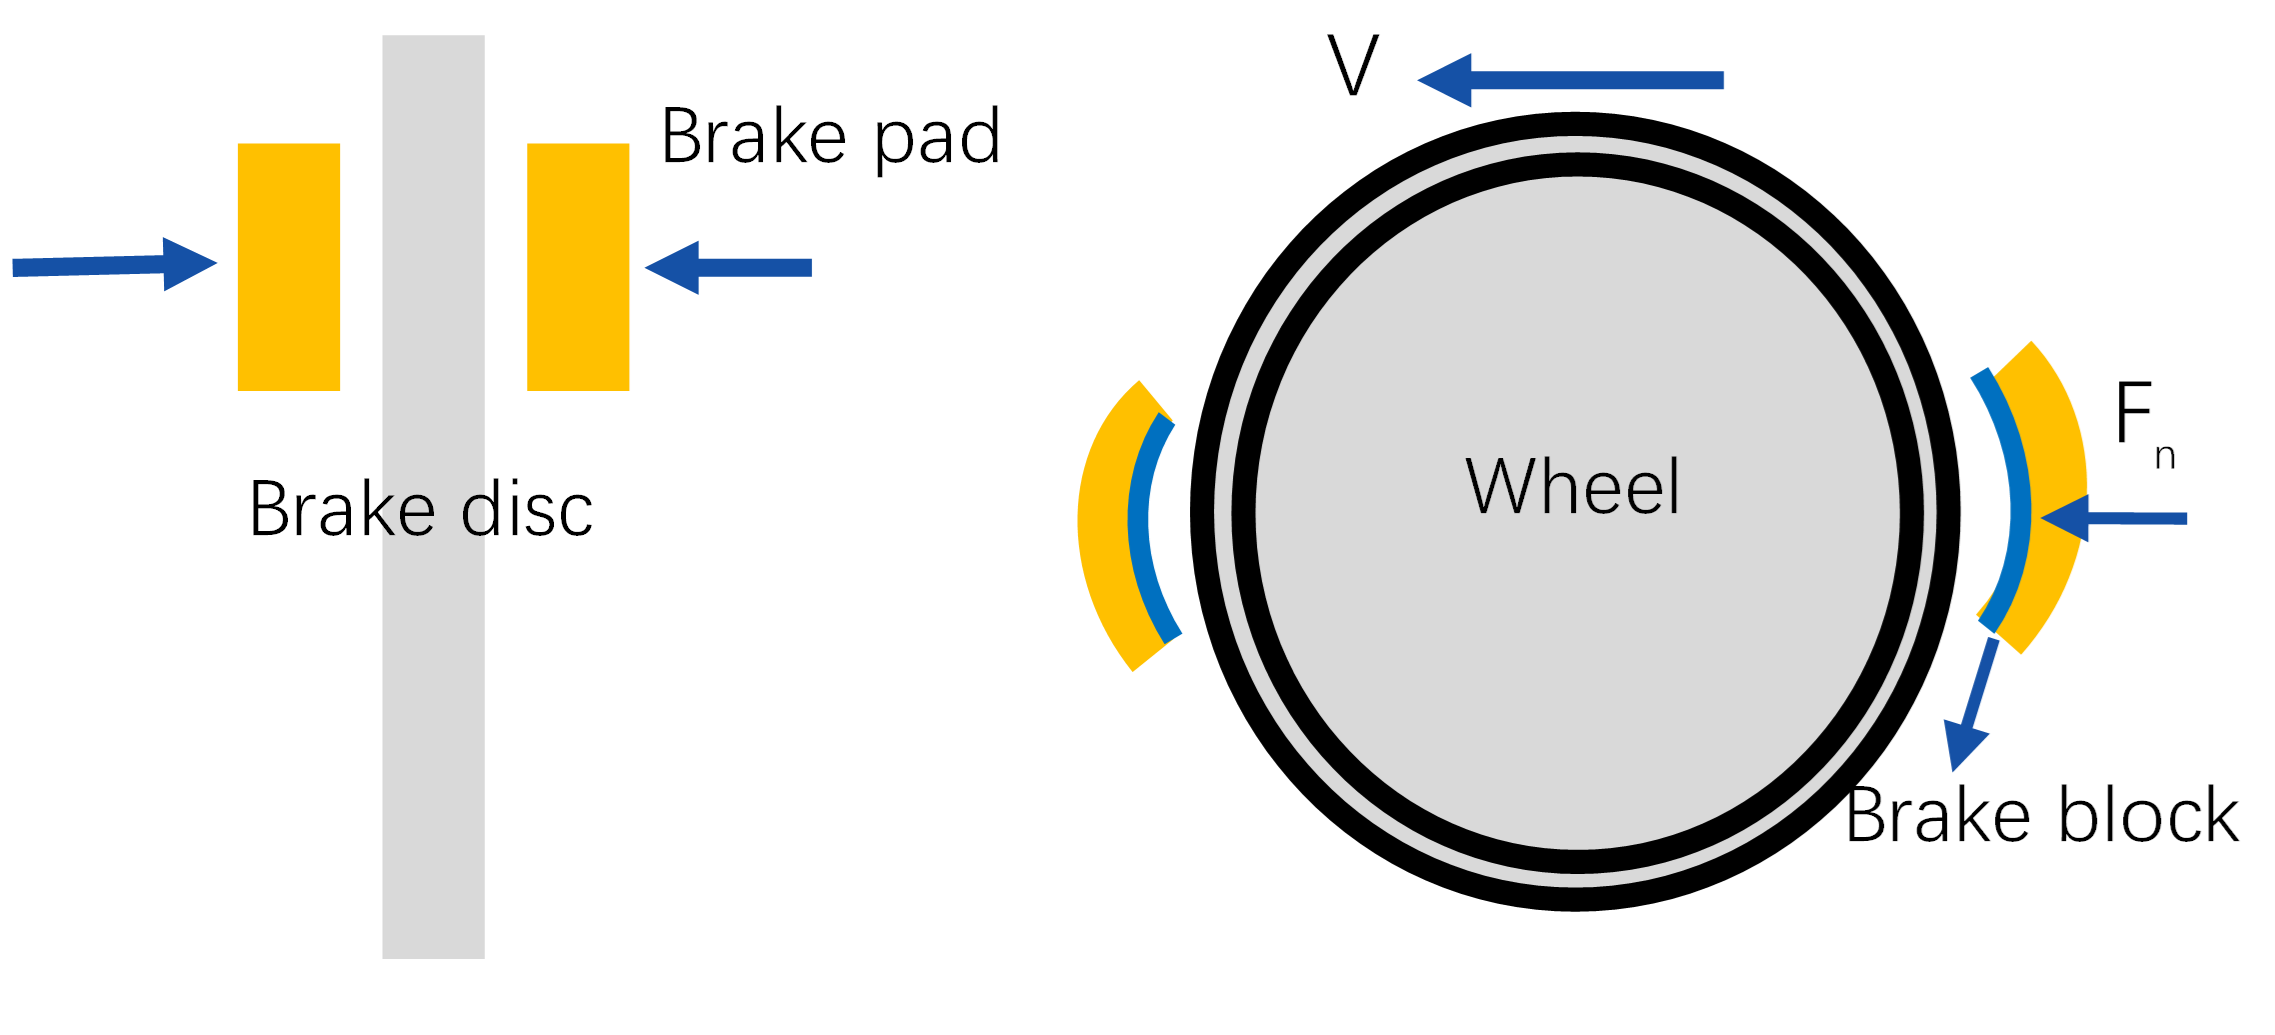
\includegraphics[width=0.65\textwidth]{book/chapters/zhang/graphics/disc_block_brakes.png}
    \caption{Block and disc brakes for rail vehicles}
    \label{fig:disc_block}
\end{figure}

Most thermal analyses of brake discs assume full contact between the brake pads and discs. From tribology studies, the real contact area is around 20\% of the whole brake pad friction surface \cite{eriksson_nature_2002}. Because of thermal expansion and wear of the brake pads, the contact area between the brake pads and discs is always changing. It is difficult to predict the true contact area. However, assuming fixed contact areas, the effect on the temperatures of brake discs can be investigated. This research aims to address the effects of different contact areas on the temperature of the brake discs.



\section*{Methods}

\subsection*{Modelling}
Heat generation and dissipation are two main parts of conducting thermal analysis of railway brake discs. Heat flux is based on friction
\begin{equation}
    q_d = \xi F_f V = \xi P A_d \mu V, 
    \label{heat flux}
\end{equation}

where \( q_d \) is the heat flux in the brake discs (W/m$^2$), \( \xi \) is the heat partition coefficient, \( F_f \) is the friction force (N), \( V \) is the velocity (m/s), \( P \) is the local contact pressure between the brake pads and discs (Pa), \( A_d \) is the friction contact area of the brake pads (m$^2$), and \( \mu \) is the coefficient of friction. Equation \ref{heat flux} is the Neumann boundary condition of Equation \ref{heat equation}, which is the overall heat transfer equation.

The heat flux distribution between the brake pads and discs is vital since it depends on how much heat flows to brake discs, which affects the temperatures and stresses. This coefficient is highly non-linear, affected by material, temperature, and pressure. In this research, this coefficient is simplified to a constant number. The distribution factor is described by \cite{rudolf_limpert_brake_1999}
\begin{equation}
    \xi = \frac{q_p}{q_d + q_p},
\end{equation}
where \( q_p \) is the heat flux in the brake pads (W/m$^2$), and \( q_d \) is the heat flux in the brake discs (W/m$^2$). 

The next step is to build a FEM model of the brake disc. FEM is a method to solve partial differential equations. This method includes the discrete domain, uses an appropriate basis, and rewrites algebraic equations. The heat equation is 
\begin{equation}
    \rho c \frac{\partial T}{\partial t} + \nabla \cdot (- k \nabla T) = f,
    \label{heat equation}
\end{equation}
where \( \rho \) is density, \( c \) is thermal capacity, \( T \) is temperature, \( t \) is time, \( k \) is the overall heat transfer coefficient, and \( f \) is the inner heat source. The time derivative on the right-hand side can be approximated by a difference quotient. Here we use the Euler backward method for consideration of numerical stability. After that, all items are multiplied by a test function \( v \) and integrated by parts. Then according to the divergence theorem, the bilinear form \( a(T,v) \) and linear form \( L(v) \) are

\begin{equation}
    a(T,v) = \frac{\rho c}{\Delta t} \int_\Omega T v dx + \int_\Omega k \nabla T \cdot \nabla v dx + \int_{\partial \Omega} h T v ds + \int_{\partial \Omega} \epsilon \sigma T^4 v ds,
\end{equation}

\begin{equation}
    L_{n+1}(v) = \int_\Omega f^{n+1} v dx 
    + \frac{\rho c}{\Delta t} \int_\Omega  T^{n} v dx 
    -  \int_{\partial \Omega} q v ds
    +  \int_{\partial \Omega} h T_a v ds 
    + \int_{\partial \Omega} \epsilon \sigma T_a^4 v ds,
\end{equation}
where \( \Omega \) is the computation domain, \( \partial \Omega \) is the boundary, \( dx \) is the differential element for integration over the domain, and \( ds \) is the differential element for integration over the boundary, \( h \) is the heat convection coefficient,  \(\Delta t\)\ is the time step, \(n\) is an integer counting time levels. The thermal radiation equation is based on Stefan-Boltzmann Law, where \( \epsilon \) is the emissivity, \( \sigma \) is Stefan-Boltzmann constant, \(T\) is the temperature and \(T^4\) is the temperature to the power of four, \( T_a \) is ambient temperature. For more detailed derivation, please see  \href{https://github.com/Yanjun96/fenicsx/blob/main/derivation_of_heat_transfer.pdf}{derivation of weak form for heat transfer equation}.

The above equation is only for heat transfer, as for brake pad deformation, one needs to solve the elastic equation and here we haven't included here. The main contribution of the elastic deformation calculation is a more accurate contact area between the brake pads and the discs. In this study, we assume that the contact area is known a priori since this research focuses on comparing the influence of different contact areas. The above equations are solved in the FEniCSx platform \cite{baratta_dolfinx_2023,scroggs_construction_2022,alnaes_unified_2014}. All the codes for this paper are in \cite{zhang_thermal_2025}.

The computation domain or mesh is shown in Figure \ref{fig:coarse mesh}. This is a much coarser mesh than the one with 1 million elements used later, with around 43,000 elements. The element type is tetrahedron since when we compared it with hexahedral elements, we found with more tetrahedron elements, the simulation can get the same accuracy with hexahedral elements while tetrahedron has less computation time. Only the brake disc and pad are computation domains. The friction heat, or the Neumann boundary condition is applied on the contact surface, more specifically, only the rubbing elements of the brake pad areas. The rubbing elements are the column structure of the brake pad. Other boundaries include radiation and convection heat transfer, which are also the Neumann boundary conditions without the heat flux input. In each time step, the boundary conditions are redefined since the rotation will change the contact area. In reality, the brake pad should keep still while the brake disc rotates. Here we assumed only the heat flux input areas are rotating: these are the friction heat input areas.

\begin{figure}[h]
    \centering
    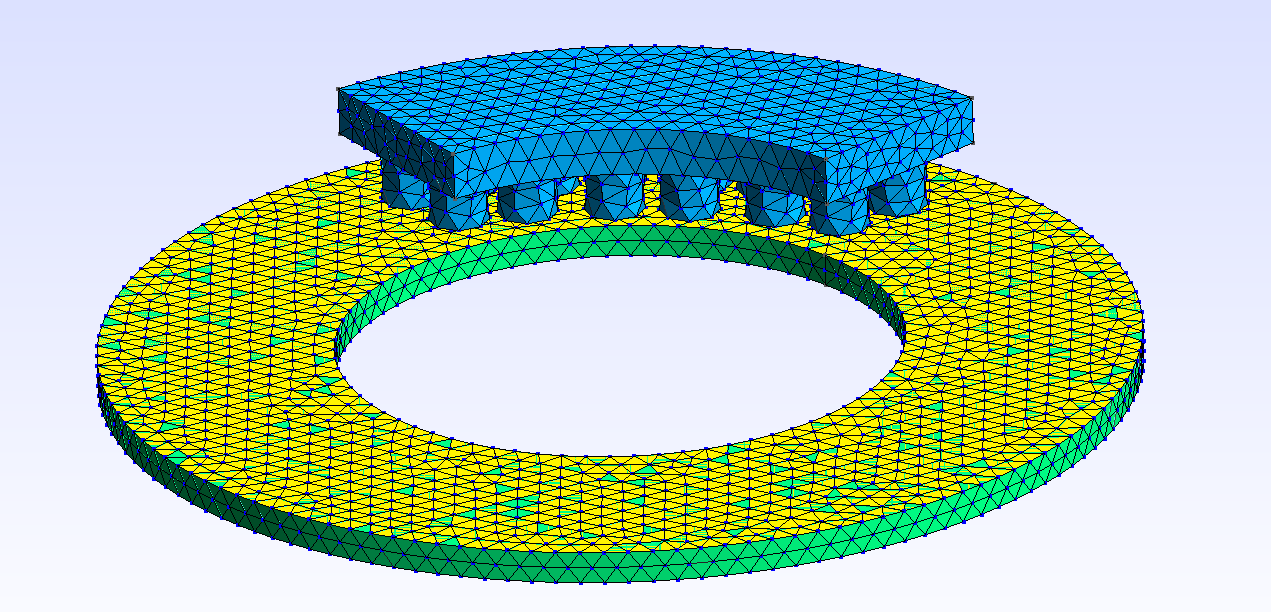
\includegraphics[width=0.9\textwidth]{book/chapters/zhang/graphics/3d surface.png}
    \caption{Computation domain of brake pad and disc, the mesh is much coarser than 1 million case. Friction heat or the Neumann boundary condition is only applied to friction contact areas.}
    \label{fig:coarse mesh}
\end{figure}


\subsection*{Experiment}

The test rig mainly consists of a DC motor, flywheels, brake pad and brake disc, as shown in Figure \ref{fig:test rig}. The maximum motor power is 450 kW, and the maximum motor torque is 4000 Nm. The brake pressure at the reservoir ranges from 0-10 Bar. 
There are in total 6 thermocouples to measure the temperature of the brake disc, which are located under the contact surface. A symmetric model is used in the simulation to save computational effort. The brake lag is the time it takes for the brake pressure to increase from 0\% to 95\% of the target pressure. In the test, the brake lag is 4±0.2 s, which follows the UIC 541-3 standard. Table \ref{tab: operational parameters} shows the operational parameters.

\begin{figure}[h]
    \centering
    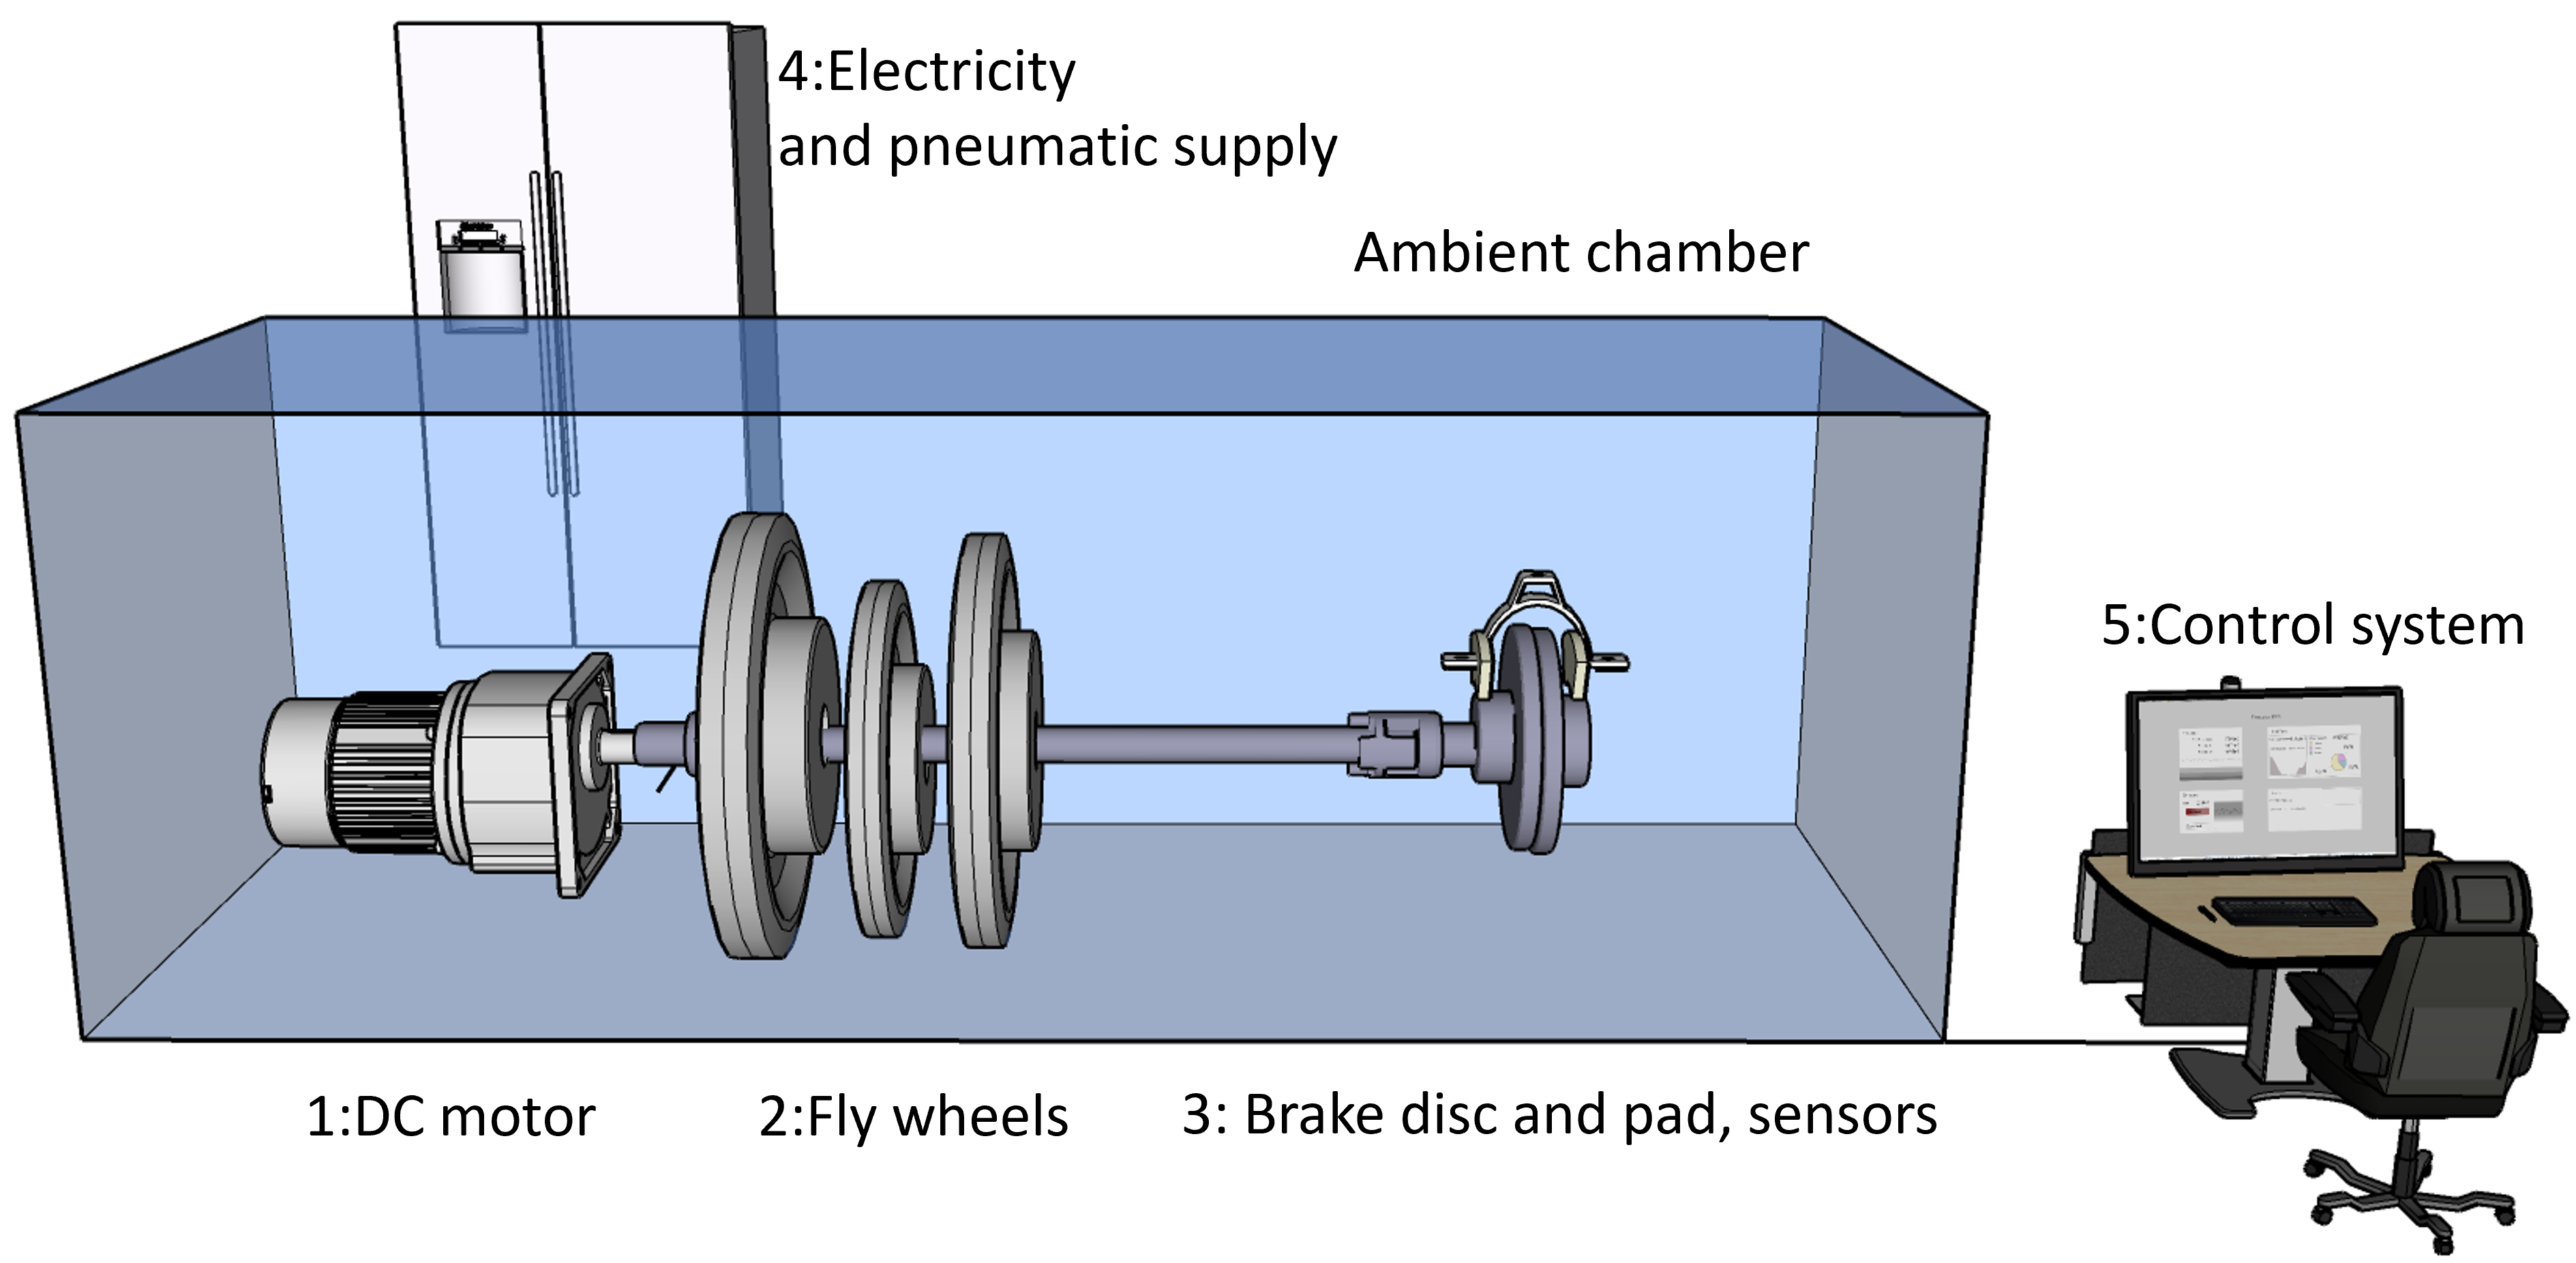
\includegraphics[width=0.85\textwidth]{book/chapters/zhang/graphics/test_rig.png}
    \caption{Full scale railway brake test rig}
    \label{fig:test rig}
\end{figure}

\begin{table}[h]
    \centering
    \begin{tabular}{llll} % 'l' for left-aligned, 'c' for centered
        \toprule
        \textbf{property} & \textbf{quantity} & \textbf{property} & \textbf{quantity}\\ % Header row
        \midrule
        initial velocity (km/h)             & 160       &braking time(s)          & 49 \\
        contact pressure (MPa)              & 0.274      &coefficient of friction  & 0.376 \\
        heat transfer coefficient( W/(m·k)) & 30-125    &heat distributor factor  & 0.88 \\
        brake lag (s)                       & 4         &initial temperature ($^\circ\text{C}$) & 50\\
       
        \bottomrule
    \end{tabular}
    \caption{Brake test parameters}
    \label{tab: operational parameters}
\end{table}

\begin{figure}[h]
    \centering
    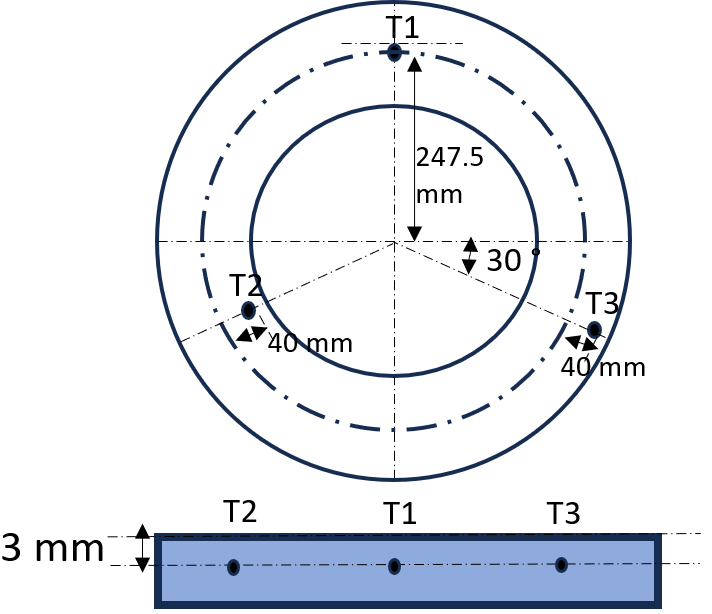
\includegraphics[width=0.45\textwidth]{book/chapters/zhang/graphics/thermo_couples.png}
    \caption{Location of three thermocouples}
    \label{fig:thermocouples}
\end{figure}


\section*{Results and discussion}

\subsection*{Validation}
The first step is mesh sensitivity and time step analysis, where we aim to show that the simulation results converge with finer mesh sizes and smaller time steps. Since no exact solution exist, the average temperature of point T1, as shown in Figure \ref{fig:thermocouples} is used as the convergence parameter.
\begin{figure}
    \centering
    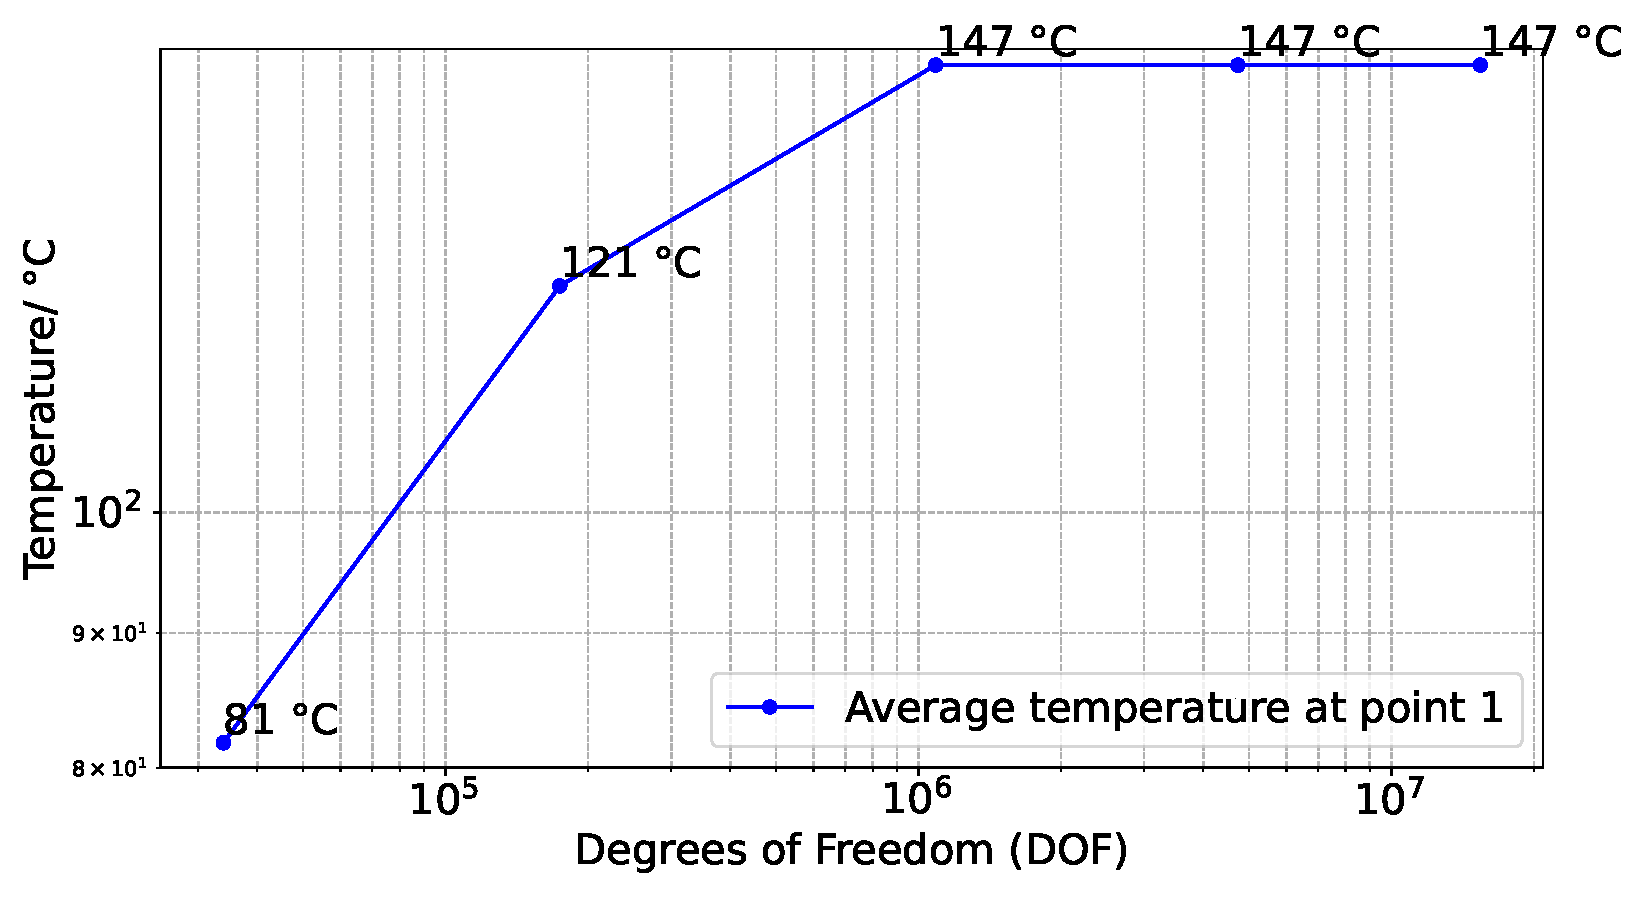
\includegraphics[width=0.8\linewidth]{book/chapters/zhang/graphics/ave_T_vs_dof.pdf}
    \caption{Convergence test, average temperatures of point T1, compared with degrees of freedom (DOFs)}
    \label{fig:error_mesh}
\end{figure}

 As shown in Figure \ref{fig:error_mesh}, the average temperature of point T1 increases with more degrees of freedom until 1 million degrees of freedom (DOFs). Above 1 million, the temperature remains constant.  The above results show that DOFs above 1 million are enough to capture the characteristics of the system. 
\begin{figure}[h]
    \centering
  
    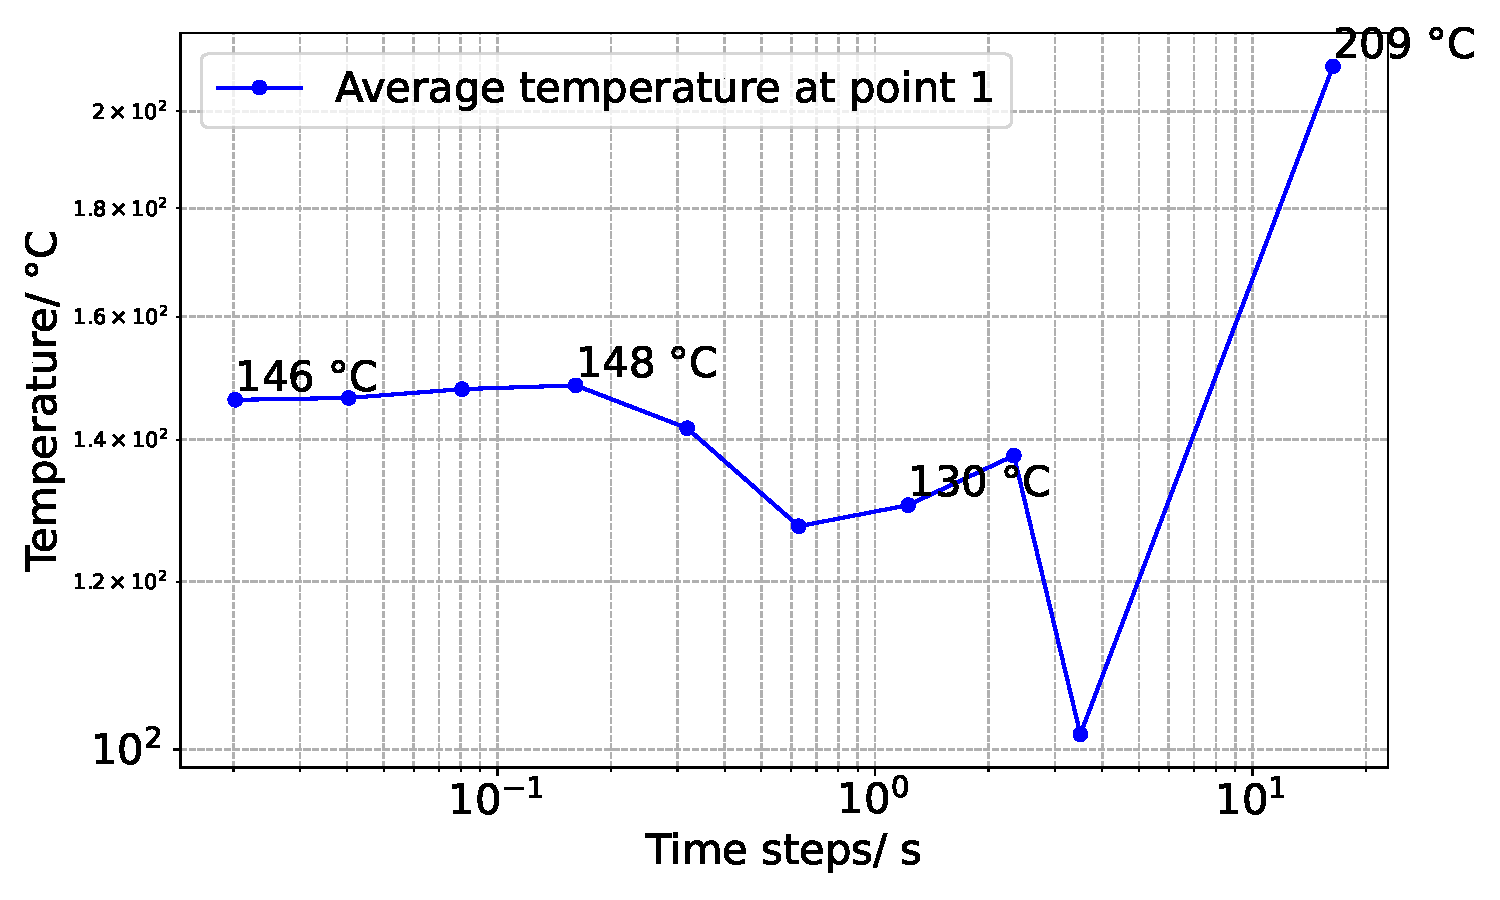
\includegraphics[width=0.8\textwidth]{book/chapters/zhang/graphics/T_ave_vs_dt.pdf}
    \caption{Convergence test, average temperatures of point T1 with time step}
    \label{fig:error_time}
\end{figure}


Figure \ref{fig:error_time} is a comparison of the average temperature of point 1 and times steps. When \(dt\) is above 1 s, the temperature has a large variance. The best value of \(dt\) is 0.16 s (point of 148$^{\circ}\text{C}$ ), which is a balance time step between accuracy and computational time.

\begin{figure}[h]
    \centering
    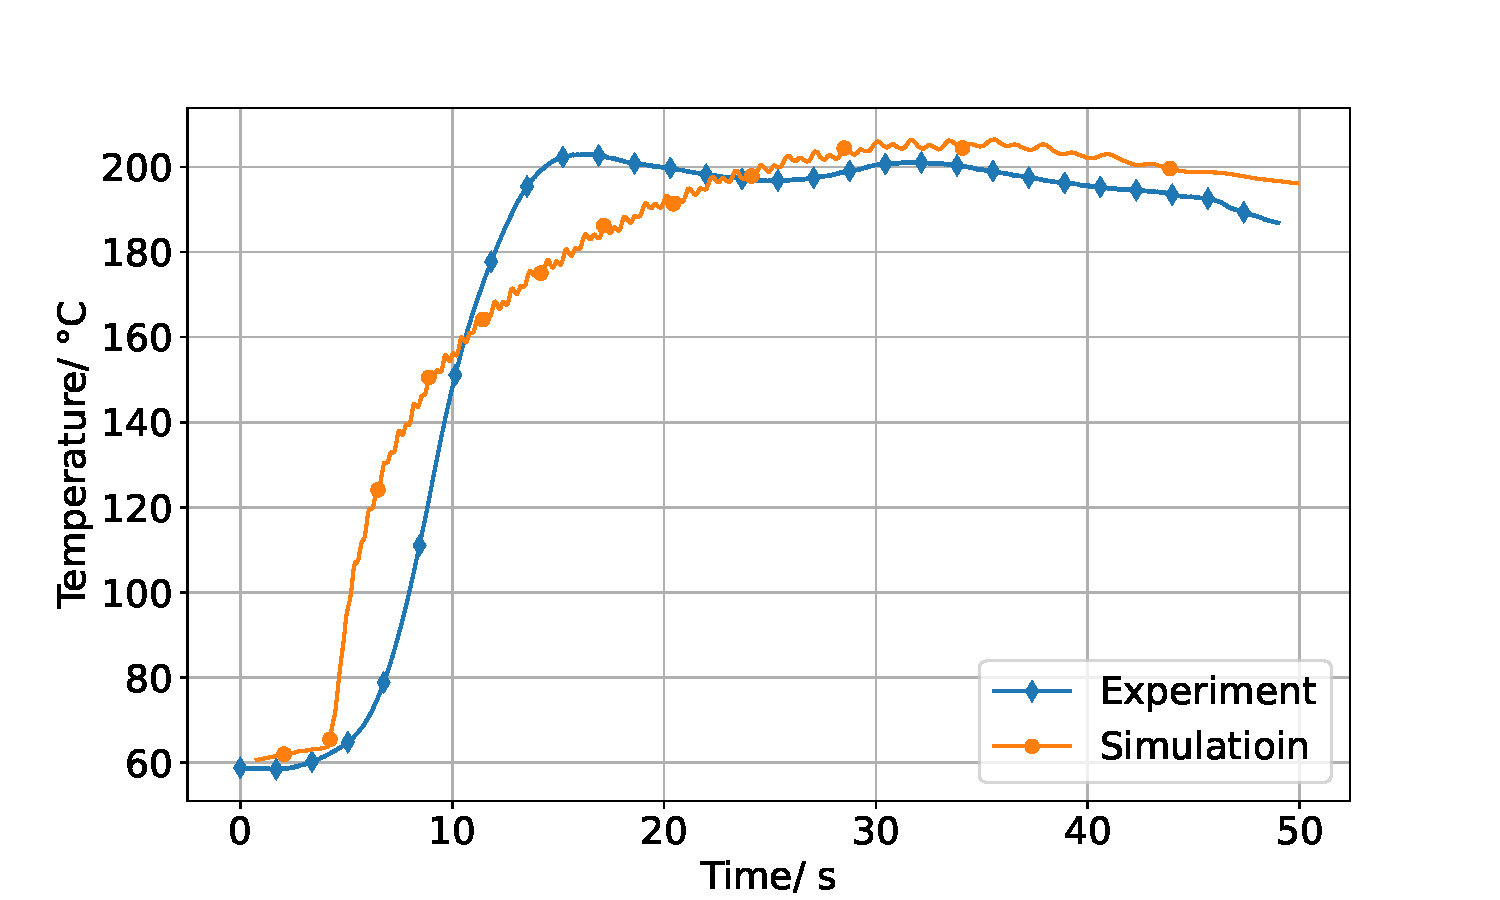
\includegraphics[width=0.8\textwidth]{book/chapters/zhang/graphics/T_sim_exe.pdf}
    \caption{Comparison between simulation time and experimental results}
    \label{fig:experiment}
\end{figure}

Except for mesh and time sensitivities analysis, the simulation results should validated against the experiment. As shown in Figure \ref{fig:experiment}. The general trend of case 1.2 million elements(4.7 million DOFs) and measurement data are the same, so we think the simulation accuracy is acceptable. However, there is still a large space to improve the accuracy. Such as introducing nonlinear material properties. These parameters, such as thermal conductivity, heat capacity, and coefficient of friction are all not constant or linear with temperature, velocity, and pressure. Getting the exact material characteristics is difficult. So better numerical results can benefit from the research of tribology and material engineering. The more detailed experiment parameters, like the loading pressure, would also significantly improve the numerical results since the experiment tests also contain large variances.



\subsection*{Average and maximum temperatures}

This section presents the temperatures of brake discs with different contact areas. The average and the maximum temperatures are presented.
The total contact surface is 200 cm$^2$. The brake pressures from the back of the brake pads are the same, 0.274 MPa, while the different contact areas will affect the contact pressure between the brake pads and discs. 20\%, 50\% and 100\% contact areas are compared. The 20\% contact areas represent the research from Eriksson \cite{eriksson_nature_2002}, and the 100\% contact areas represent most FEM or analytical solutions.

\begin{figure}[h]
    \centering
    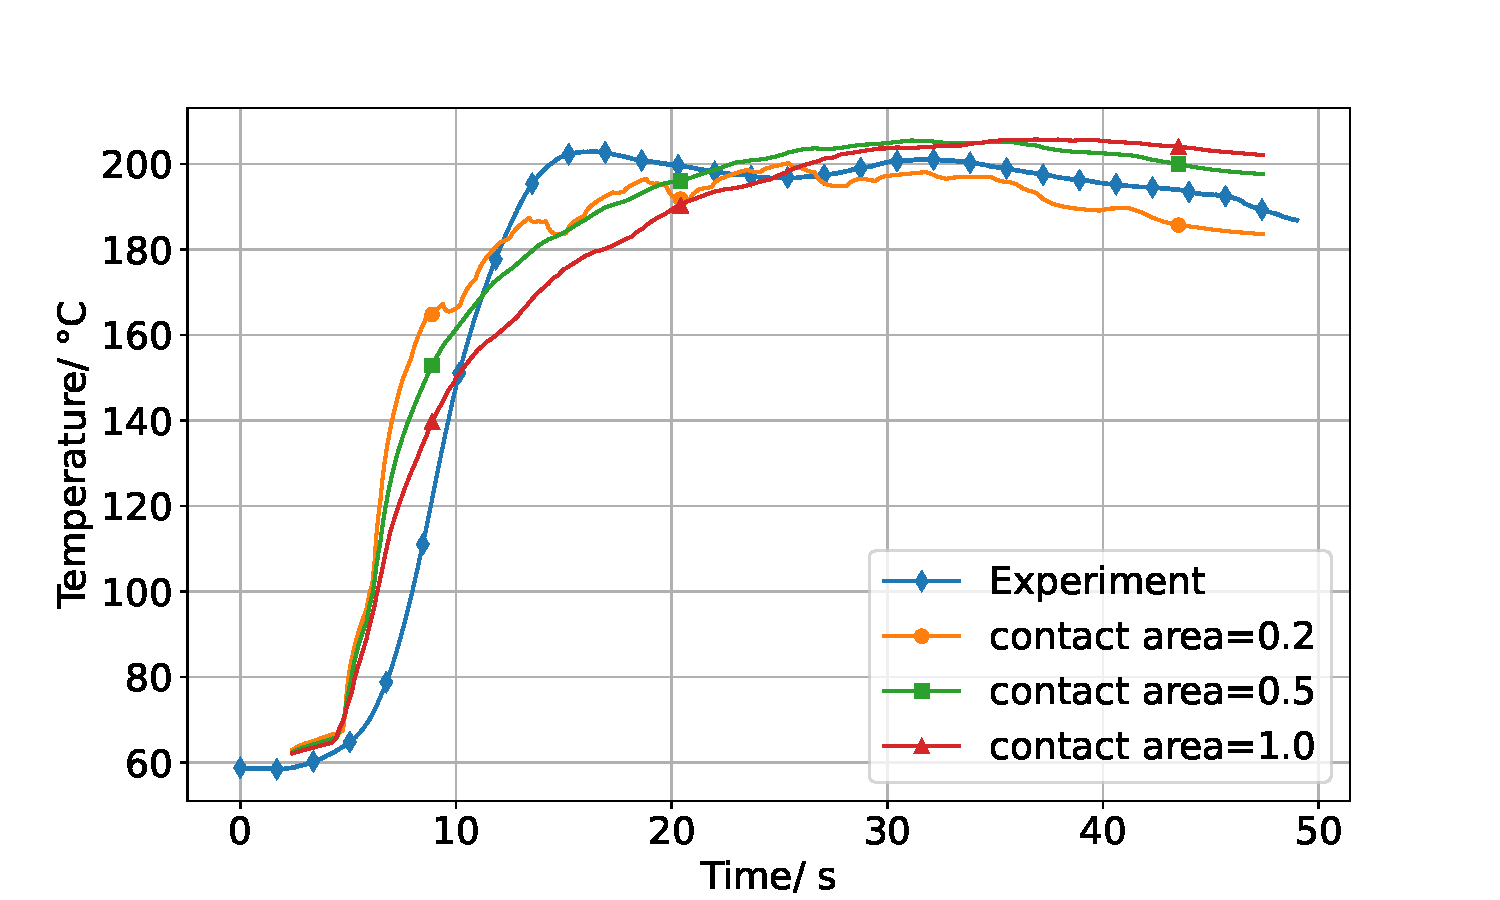
\includegraphics[width=0.8\textwidth]{book/chapters/zhang/graphics/T_ave_dc.pdf}
    \caption{Average temperatures with different contact areas}
    \label{fig:T_ave}
\end{figure}

As shown in Figure \ref{fig:T_ave} is the average temperature for these three cases. The maximum temperature difference is 20 $^{\circ}\text{C}$ between 20\% and 100\% contact areas. The maximum relative difference is 16.6\%. The average temperature is not sensitive to different contact areas since the total heat input is the same, while only heat dissipation is slightly different because the temperature distribution of the brake discs is uneven. Uneven temperature distribution can be proven through the comparison of the maximum temperatures.

\begin{figure}[h]
    \centering
    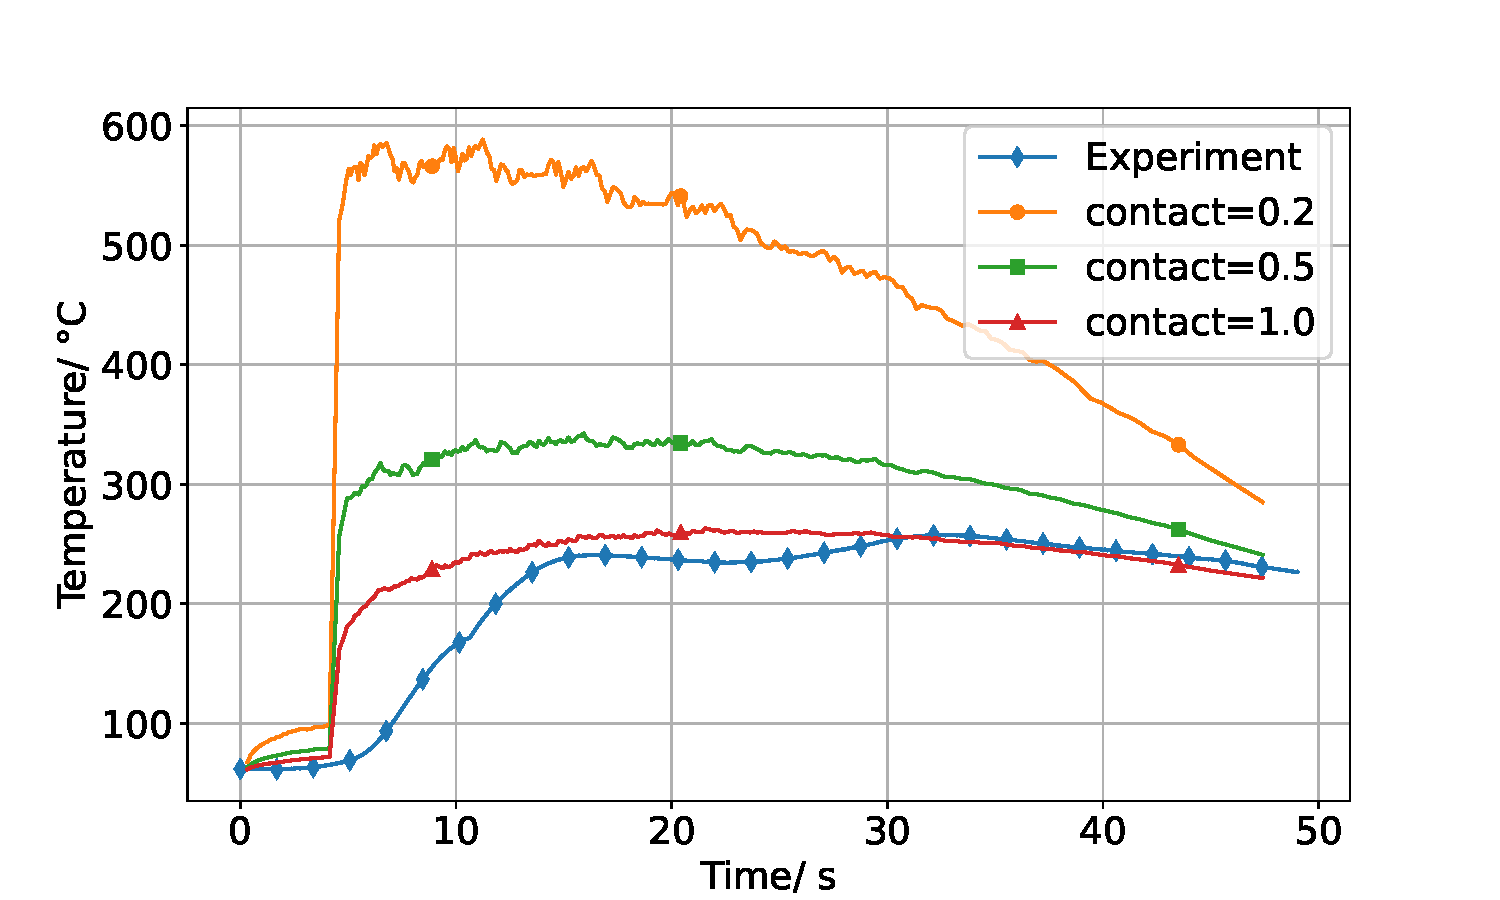
\includegraphics[width=0.8\textwidth]{book/chapters/zhang/graphics/T_max_dc.pdf}
    \caption{The maximum temperatures with different contact areas}
    \label{fig:T_max}
\end{figure}

Figure \ref{fig:T_max} shows the maximum temperature of the brake discs. The maximum temperature difference is more than 300 $^{\circ}\text{C}$, and the relative difference can reach 160\%. Small contact areas induce higher local temperatures since contact pressure is significantly increased and all friction heat is loaded on limited surfaces.

More advanced research can be conducted based on this FEM model, including sensitivity analysis of railway brake disc temperature development. In the future, the following need to be considered to build a more realistic model to investigate different brake designs:

\begin{enumerate}
\item Coupling elastic equations to get deformation details of the brake pads.
\item Considering more nonlinear parameters, like a variable coefficient of friction, and temperature-dependent material properties.
\end{enumerate}


\section*{Conclusion}
This study investigates the influence of contact area on the temperature of railway brake discs. A FEM model in FEniCSx is built and validated. The following conclusions can be drawn:
\begin{enumerate}
\item The contact area does not influence average temperature significantly while a small contact area induces a higher maximum temperature.
\item FEM based research on thermal analysis of brake systems should model real contact areas between brake pads and discs to get an accurate temperature distribution.
\end{enumerate}


\begin{acknowledgement}
This work is sponsored by the KTH Railway Group, China Scholarship Council and CRRC ZELC. Thanks to the experimental support of Fei Gao, Junying Yang at Dalian Jiaotong University. The help of Jørgen S. Dokken from the FEniCSx community and Jing Gong from Kungliga Tekniska Högskolans PDC support are especially acknowledged. Thanks to the National Academic Infrastructure for Supercomputing in Sweden for providing computer resources.        
\end{acknowledgement}

\bibliographystyle{spbasic}
% Write the full path of your bibfile relative to book.tex

\bibliography{chapters/zhang/bibliography.bib}


 
% Write the full path to the location of the graphics relative to book.tex
\graphicspath{{chapters/zhang/graphics/}}


\title{Thermal analysis of brake discs in rail vehicles}
\titlerunning{Thermal analysis}

\author{Yanjun Zhang, Sebastian Stichel and William Liu}
\authorrunning{Yanjun et al.}

\institute{Yanjun Zhang \email{yanjunzh@kth.se} \at KTH Royal Institute of Technology}

\maketitle

\abstract{}
Railway brake discs convert the kinetic energy of rail vehicles to thermal energy to achieve braking. This thermal energy deteriorates braking performance, therefore, it is necessary to conduct thermal analyses of brake discs. In this work, we build a FEM (finite element method) model in FEniCSx to investigate the influence of contact areas between brake pads and discs on the temperature of brake discs. The weak form of the nonlinear heat transfer equation has been derived, which accounts for conduction, convection and radiation. Multiple Neumann boundary conditions are applied. Simulation results are validated with experimental results. With this efficient FEM model, more advanced research related to railway brake discs can be conducted, such as investigating the effect of wear and thermal expansion, or designing a new geometry of the brake pads and discs.

\section*{Introduction}
Rail vehicles are developed towards higher speed and higher axle load, requiring robust mechanical brake systems for running safety. As shown in figure \ref{fig:disc_block}, one of the most important mechanical brake systems is the disc brake, which converts the kinetic energy of the rail vehicle into heat. A high brake disc temperature reduces the coefficient of friction between the brake discs and the brake pads \cite{Saffar2010}, and causes high thermal stress, which, in turn, induces thermal cracks on the brake discs. To avoid these negative impacts, it is necessary to study the temperature distribution of brake discs. Experimental investigation is relatively complex and can not obtain some parameters, while numerical study is an effective way to address this issue.

\begin{figure}[h]
    \centering
    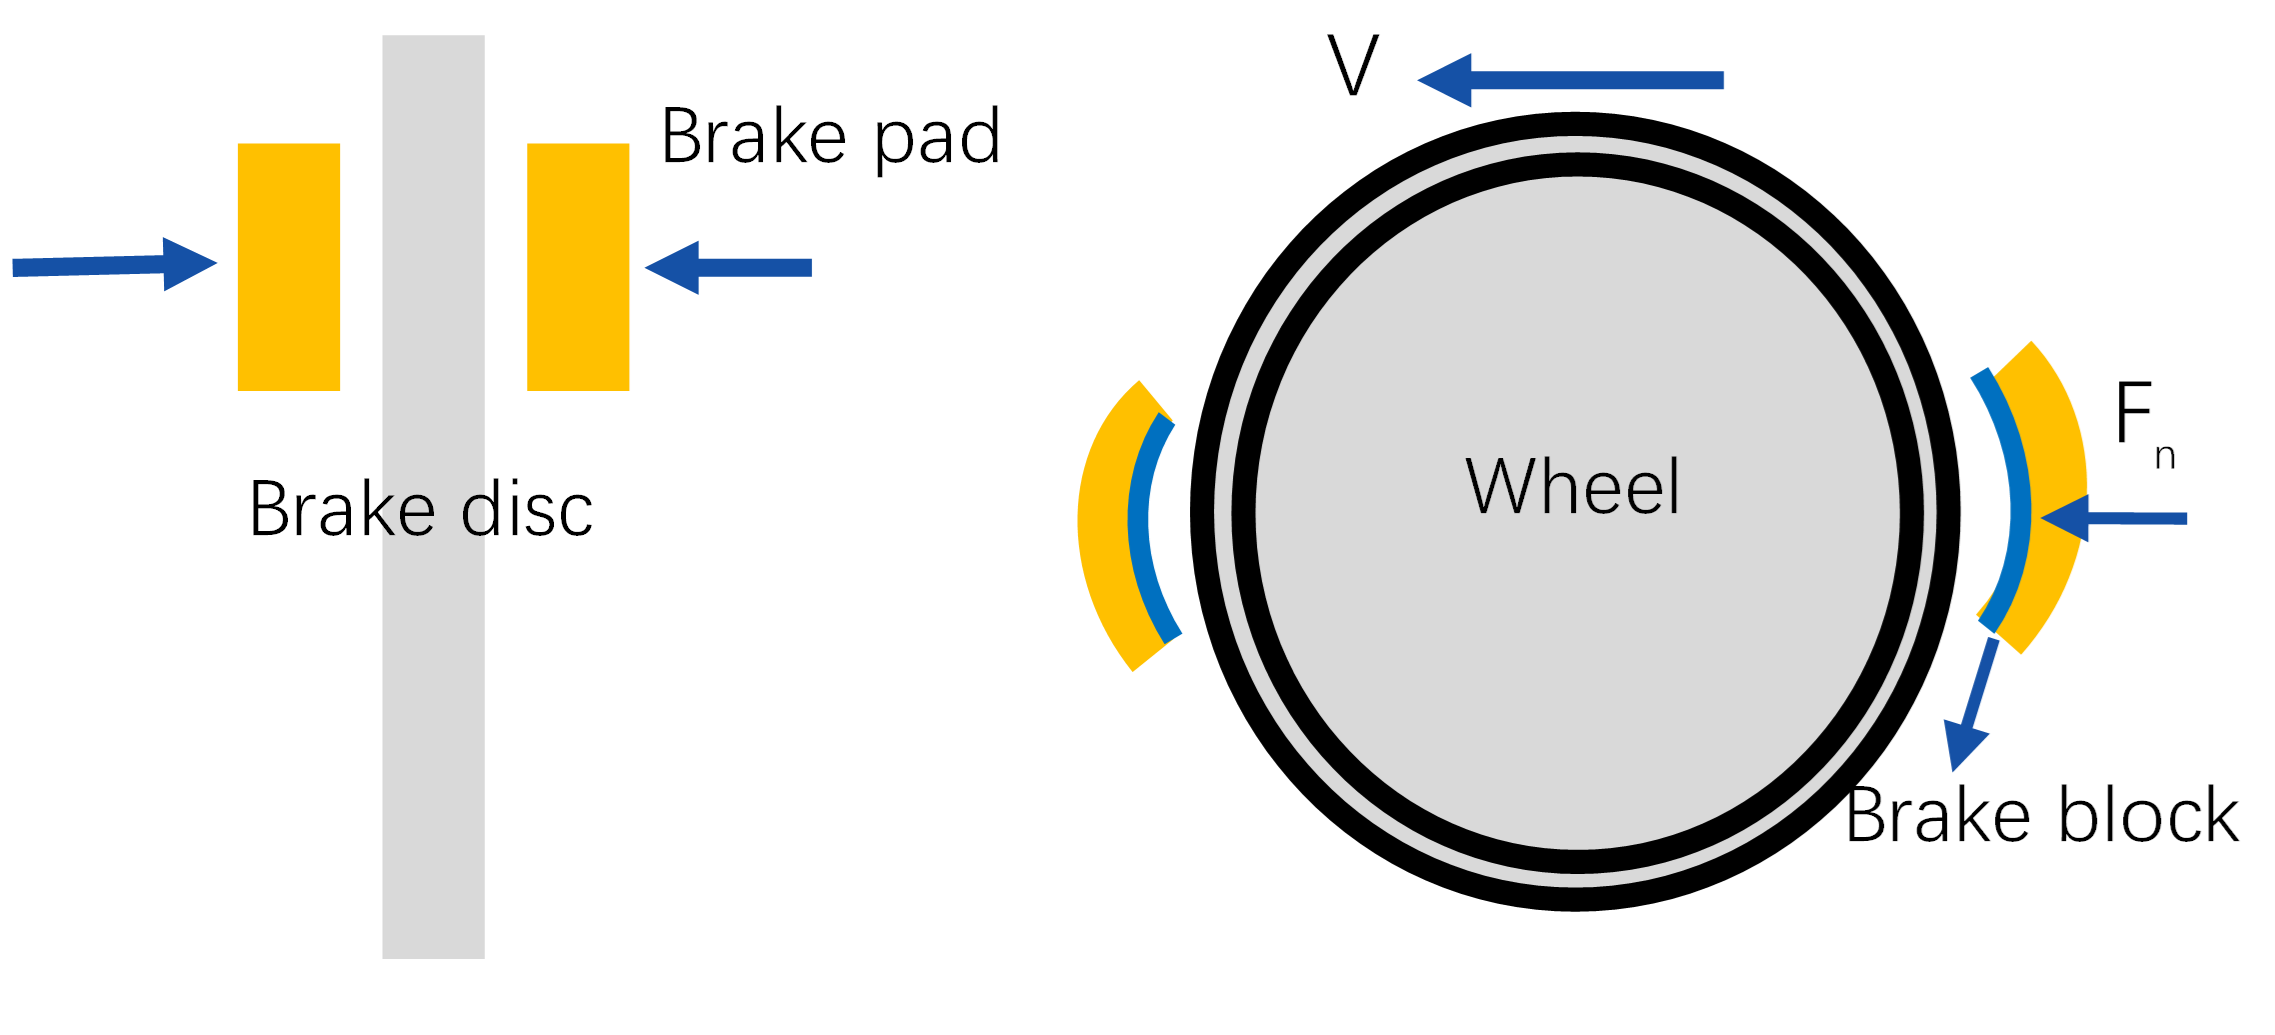
\includegraphics[width=0.65\textwidth]{book/chapters/zhang/graphics/disc_block_brakes.png}
    \caption{Block and disc brakes for rail vehicles}
    \label{fig:disc_block}
\end{figure}

Most thermal analyses of brake discs assume full contact between the brake pads and discs. From tribology studies, the real contact area is around 20\% of the whole brake pad friction surface \cite{eriksson_nature_2002}. Because of thermal expansion and wear of the brake pads, the contact area between the brake pads and discs is always changing. It is difficult to predict the true contact area. However, assuming fixed contact areas, the effect on the temperatures of brake discs can be investigated. This research aims to address the effects of different contact areas on the temperature of the brake discs.



\section*{Methods}

\subsection*{Modelling}
Heat generation and dissipation are two main parts of conducting thermal analysis of railway brake discs. Heat flux is based on friction
\begin{equation}
    q_d = \xi F_f V = \xi P A_d \mu V, 
    \label{heat flux}
\end{equation}

where \( q_d \) is the heat flux in the brake discs (W/m$^2$), \( \xi \) is the heat partition coefficient, \( F_f \) is the friction force (N), \( V \) is the velocity (m/s), \( P \) is the local contact pressure between the brake pads and discs (Pa), \( A_d \) is the friction contact area of the brake pads (m$^2$), and \( \mu \) is the coefficient of friction. Equation \ref{heat flux} is the Neumann boundary condition of Equation \ref{heat equation}, which is the overall heat transfer equation.

The heat flux distribution between the brake pads and discs is vital since it depends on how much heat flows to brake discs, which affects the temperatures and stresses. This coefficient is highly non-linear, affected by material, temperature, and pressure. In this research, this coefficient is simplified to a constant number. The distribution factor is described by \cite{rudolf_limpert_brake_1999}
\begin{equation}
    \xi = \frac{q_p}{q_d + q_p},
\end{equation}
where \( q_p \) is the heat flux in the brake pads (W/m$^2$), and \( q_d \) is the heat flux in the brake discs (W/m$^2$). 

The next step is to build a FEM model of the brake disc. FEM is a method to solve partial differential equations. This method includes the discrete domain, uses an appropriate basis, and rewrites algebraic equations. The heat equation is 
\begin{equation}
    \rho c \frac{\partial T}{\partial t} + \nabla \cdot (- k \nabla T) = f,
    \label{heat equation}
\end{equation}
where \( \rho \) is density, \( c \) is thermal capacity, \( T \) is temperature, \( t \) is time, \( k \) is the overall heat transfer coefficient, and \( f \) is the inner heat source. The time derivative on the right-hand side can be approximated by a difference quotient. Here we use the Euler backward method for consideration of numerical stability. After that, all items are multiplied by a test function \( v \) and integrated by parts. Then according to the divergence theorem, the bilinear form \( a(T,v) \) and linear form \( L(v) \) are

\begin{equation}
    a(T,v) = \frac{\rho c}{\Delta t} \int_\Omega T v dx + \int_\Omega k \nabla T \cdot \nabla v dx + \int_{\partial \Omega} h T v ds + \int_{\partial \Omega} \epsilon \sigma T^4 v ds,
\end{equation}

\begin{equation}
    L_{n+1}(v) = \int_\Omega f^{n+1} v dx 
    + \frac{\rho c}{\Delta t} \int_\Omega  T^{n} v dx 
    -  \int_{\partial \Omega} q v ds
    +  \int_{\partial \Omega} h T_a v ds 
    + \int_{\partial \Omega} \epsilon \sigma T_a^4 v ds,
\end{equation}
where \( \Omega \) is the computation domain, \( \partial \Omega \) is the boundary, \( dx \) is the differential element for integration over the domain, and \( ds \) is the differential element for integration over the boundary, \( h \) is the heat convection coefficient,  \(\Delta t\)\ is the time step, \(n\) is an integer counting time levels. The thermal radiation equation is based on Stefan-Boltzmann Law, where \( \epsilon \) is the emissivity, \( \sigma \) is Stefan-Boltzmann constant, \(T\) is the temperature and \(T^4\) is the temperature to the power of four, \( T_a \) is ambient temperature. For more detailed derivation, please see  \href{https://github.com/Yanjun96/fenicsx/blob/main/derivation_of_heat_transfer.pdf}{derivation of weak form for heat transfer equation}.

The above equation is only for heat transfer, as for brake pad deformation, one needs to solve the elastic equation and here we haven't included here. The main contribution of the elastic deformation calculation is a more accurate contact area between the brake pads and the discs. In this study, we assume that the contact area is known a priori since this research focuses on comparing the influence of different contact areas. The above equations are solved in the FEniCSx platform \cite{baratta_dolfinx_2023,scroggs_construction_2022,alnaes_unified_2014}. All the codes for this paper are in \cite{zhang_thermal_2025}.

The computation domain or mesh is shown in Figure \ref{fig:coarse mesh}. This is a much coarser mesh than the one with 1 million elements used later, with around 43,000 elements. The element type is tetrahedron since when we compared it with hexahedral elements, we found with more tetrahedron elements, the simulation can get the same accuracy with hexahedral elements while tetrahedron has less computation time. Only the brake disc and pad are computation domains. The friction heat, or the Neumann boundary condition is applied on the contact surface, more specifically, only the rubbing elements of the brake pad areas. The rubbing elements are the column structure of the brake pad. Other boundaries include radiation and convection heat transfer, which are also the Neumann boundary conditions without the heat flux input. In each time step, the boundary conditions are redefined since the rotation will change the contact area. In reality, the brake pad should keep still while the brake disc rotates. Here we assumed only the heat flux input areas are rotating: these are the friction heat input areas.

\begin{figure}[h]
    \centering
    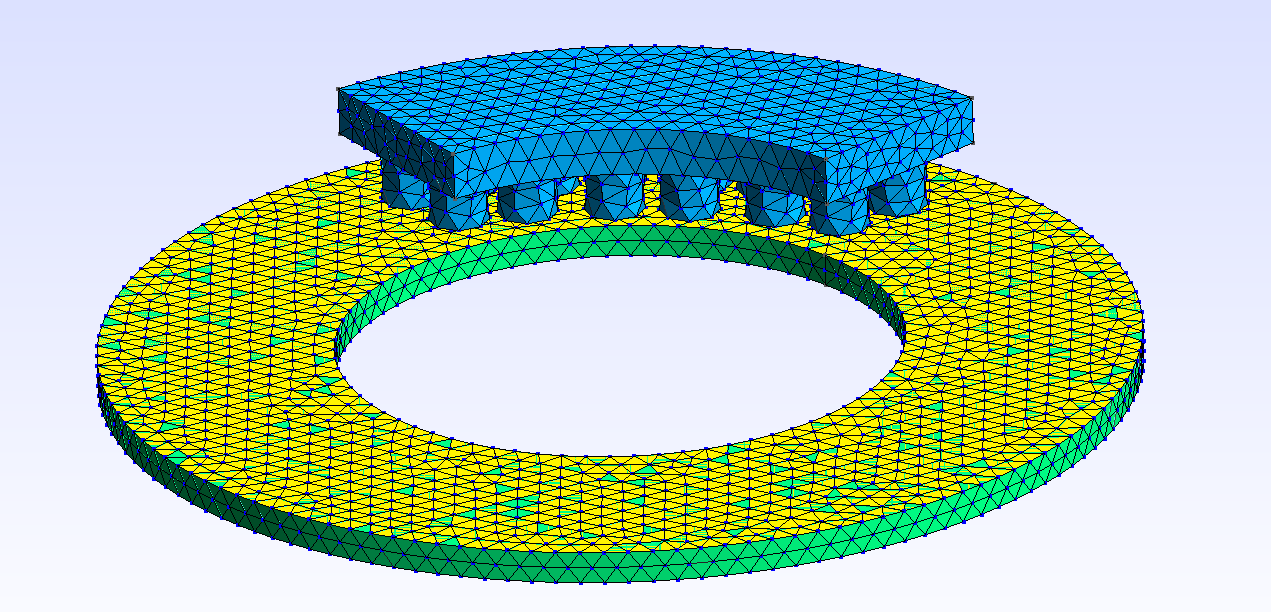
\includegraphics[width=0.9\textwidth]{book/chapters/zhang/graphics/3d surface.png}
    \caption{Computation domain of brake pad and disc, the mesh is much coarser than 1 million case. Friction heat or the Neumann boundary condition is only applied to friction contact areas.}
    \label{fig:coarse mesh}
\end{figure}


\subsection*{Experiment}

The test rig mainly consists of a DC motor, flywheels, brake pad and brake disc, as shown in Figure \ref{fig:test rig}. The maximum motor power is 450 kW, and the maximum motor torque is 4000 Nm. The brake pressure at the reservoir ranges from 0-10 Bar. 
There are in total 6 thermocouples to measure the temperature of the brake disc, which are located under the contact surface. A symmetric model is used in the simulation to save computational effort. The brake lag is the time it takes for the brake pressure to increase from 0\% to 95\% of the target pressure. In the test, the brake lag is 4±0.2 s, which follows the UIC 541-3 standard. Table \ref{tab: operational parameters} shows the operational parameters.

\begin{figure}[h]
    \centering
    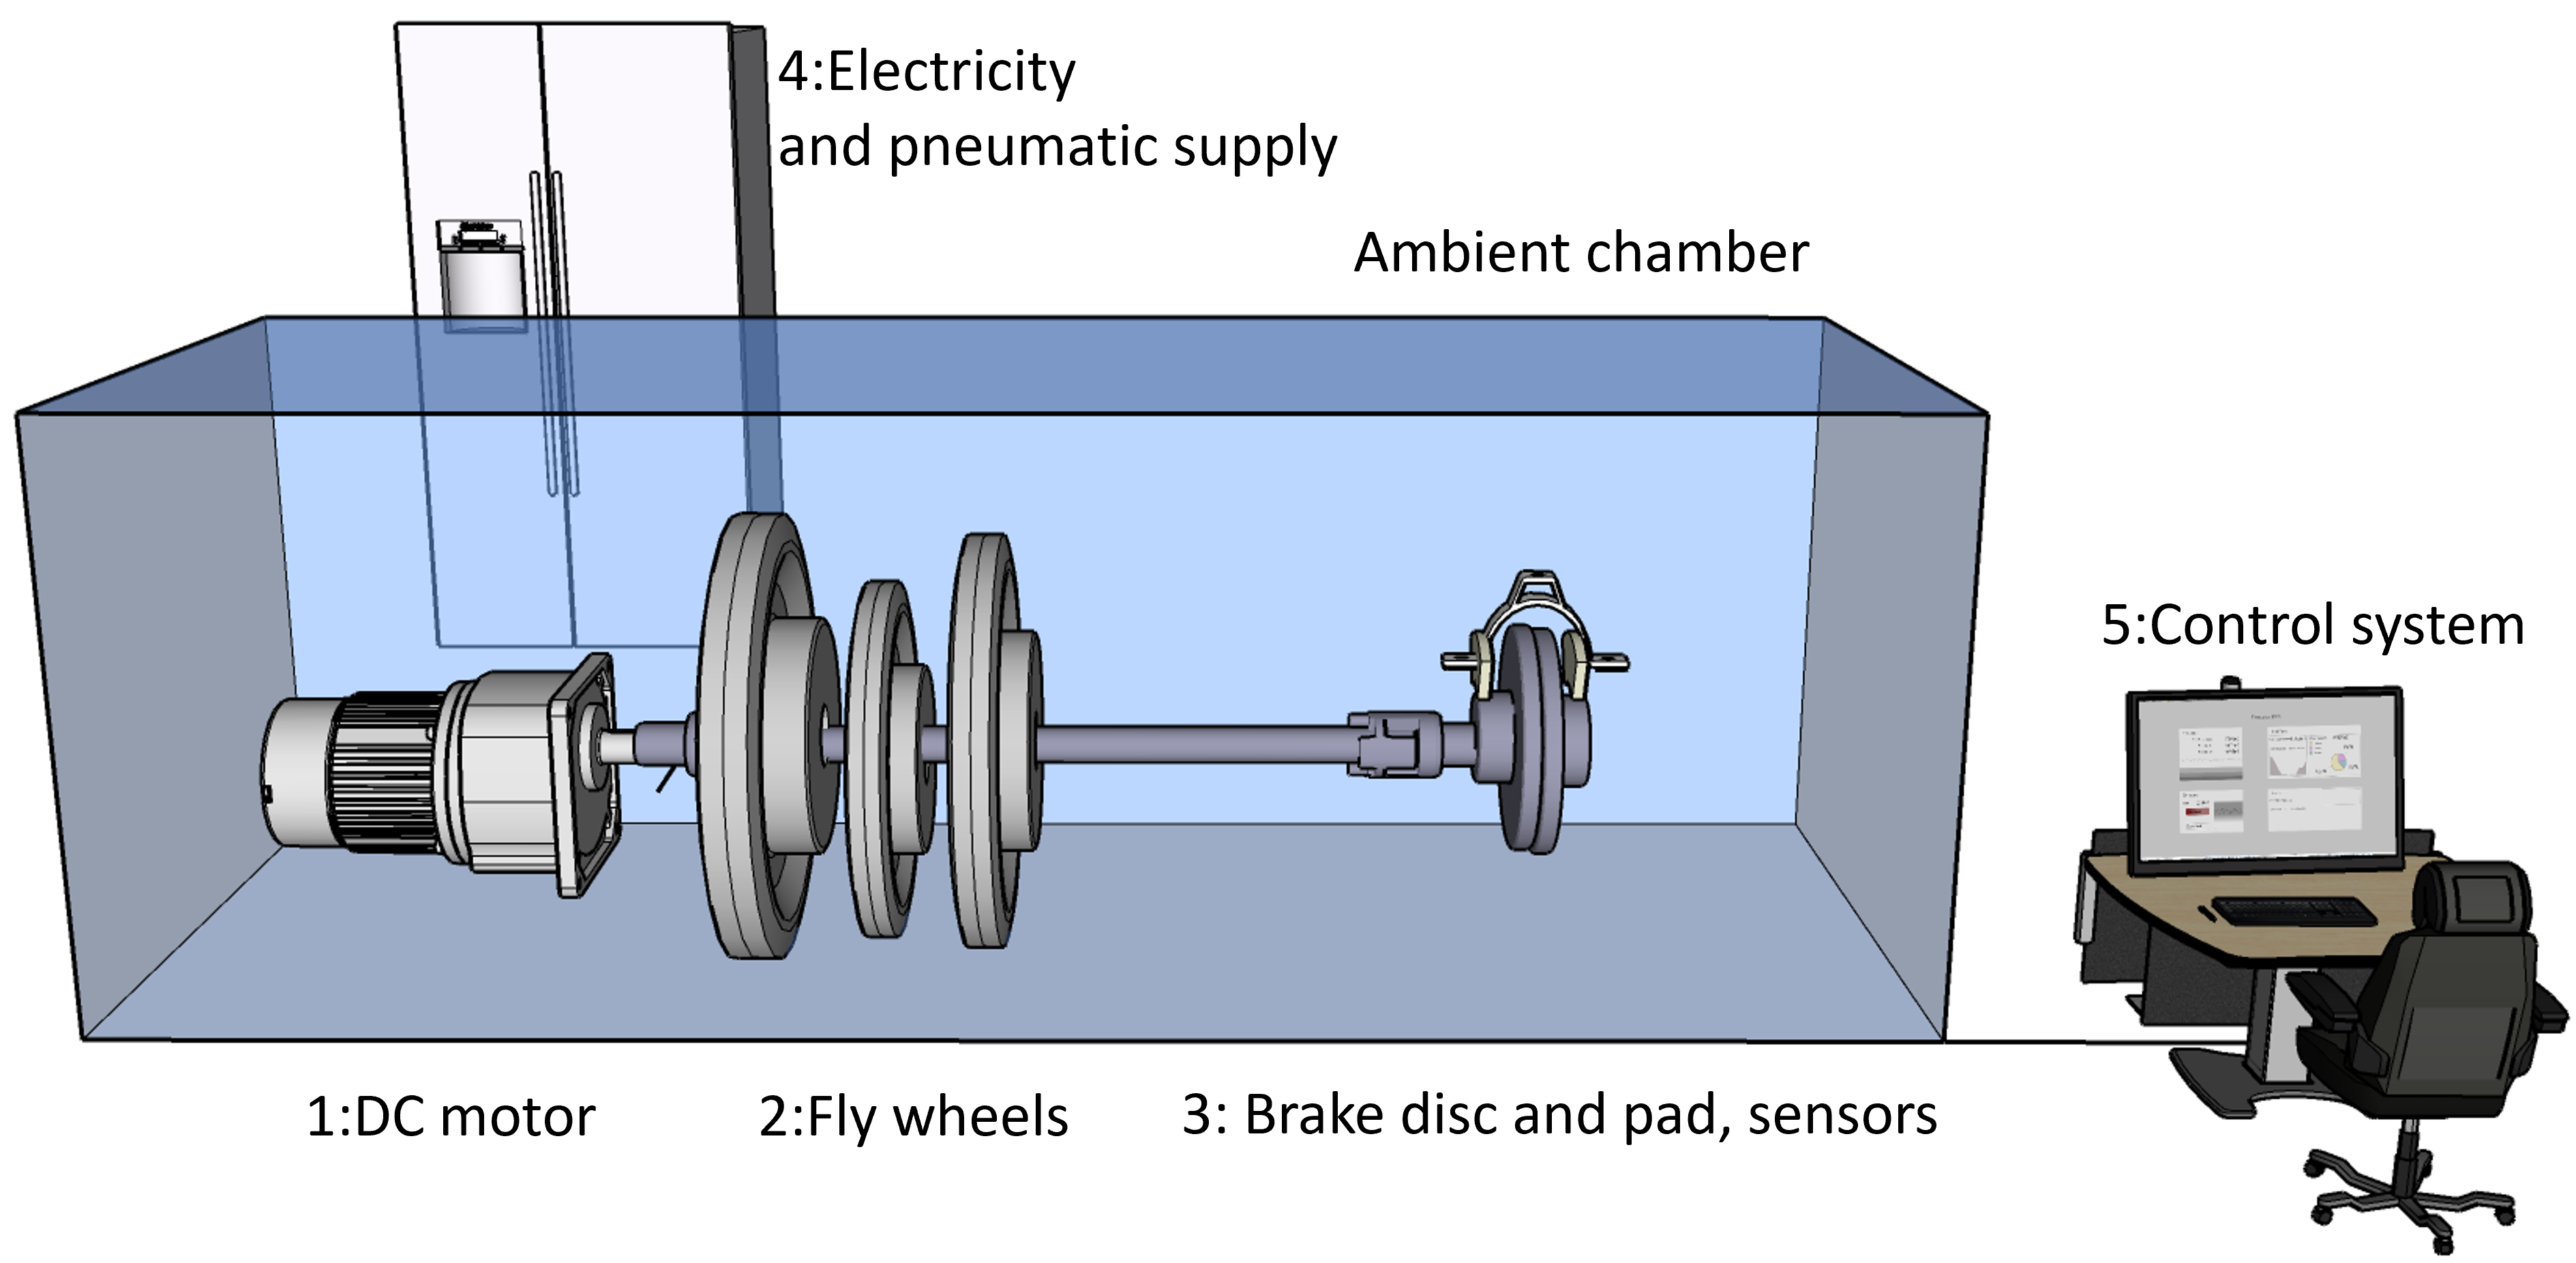
\includegraphics[width=0.85\textwidth]{book/chapters/zhang/graphics/test_rig.png}
    \caption{Full scale railway brake test rig}
    \label{fig:test rig}
\end{figure}

\begin{table}[h]
    \centering
    \begin{tabular}{llll} % 'l' for left-aligned, 'c' for centered
        \toprule
        \textbf{property} & \textbf{quantity} & \textbf{property} & \textbf{quantity}\\ % Header row
        \midrule
        initial velocity (km/h)             & 160       &braking time(s)          & 49 \\
        contact pressure (MPa)              & 0.274      &coefficient of friction  & 0.376 \\
        heat transfer coefficient( W/(m·k)) & 30-125    &heat distributor factor  & 0.88 \\
        brake lag (s)                       & 4         &initial temperature ($^\circ\text{C}$) & 50\\
       
        \bottomrule
    \end{tabular}
    \caption{Brake test parameters}
    \label{tab: operational parameters}
\end{table}

\begin{figure}[h]
    \centering
    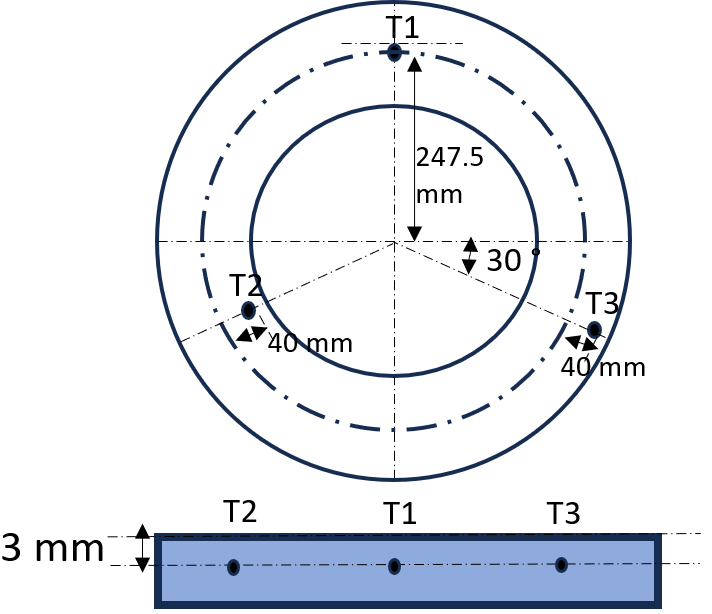
\includegraphics[width=0.45\textwidth]{book/chapters/zhang/graphics/thermo_couples.png}
    \caption{Location of three thermocouples}
    \label{fig:thermocouples}
\end{figure}


\section*{Results and discussion}

\subsection*{Validation}
The first step is mesh sensitivity and time step analysis, where we aim to show that the simulation results converge with finer mesh sizes and smaller time steps. Since no exact solution exist, the average temperature of point T1, as shown in Figure \ref{fig:thermocouples} is used as the convergence parameter.
\begin{figure}
    \centering
    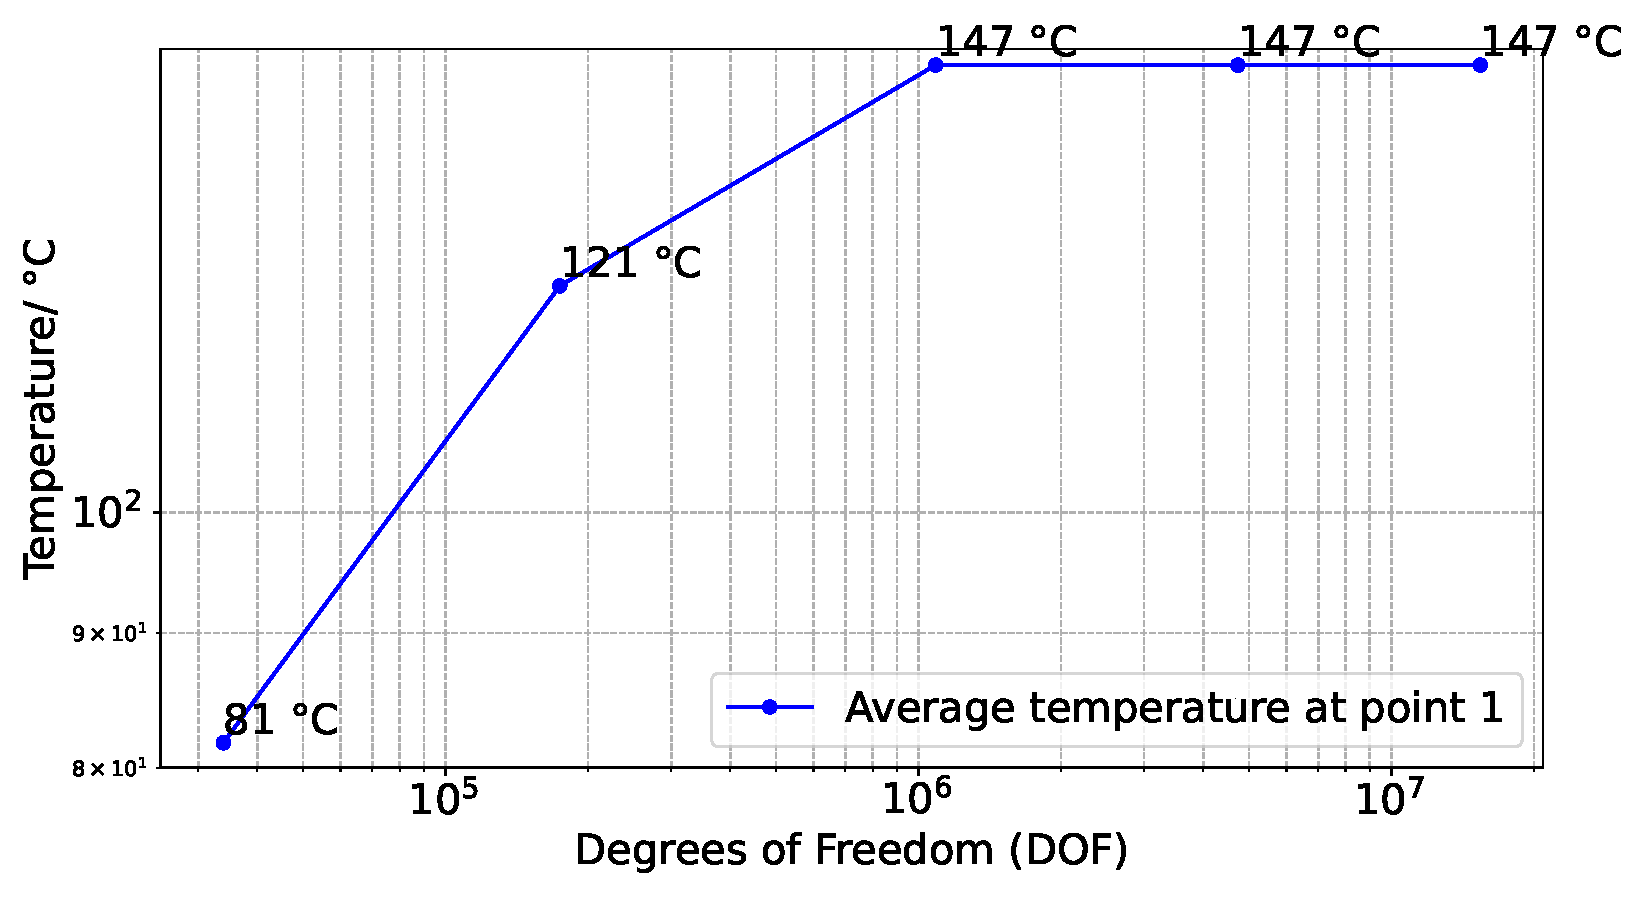
\includegraphics[width=0.8\linewidth]{book/chapters/zhang/graphics/ave_T_vs_dof.pdf}
    \caption{Convergence test, average temperatures of point T1, compared with degrees of freedom (DOFs)}
    \label{fig:error_mesh}
\end{figure}

 As shown in Figure \ref{fig:error_mesh}, the average temperature of point T1 increases with more degrees of freedom until 1 million degrees of freedom (DOFs). Above 1 million, the temperature remains constant.  The above results show that DOFs above 1 million are enough to capture the characteristics of the system. 
\begin{figure}[h]
    \centering
  
    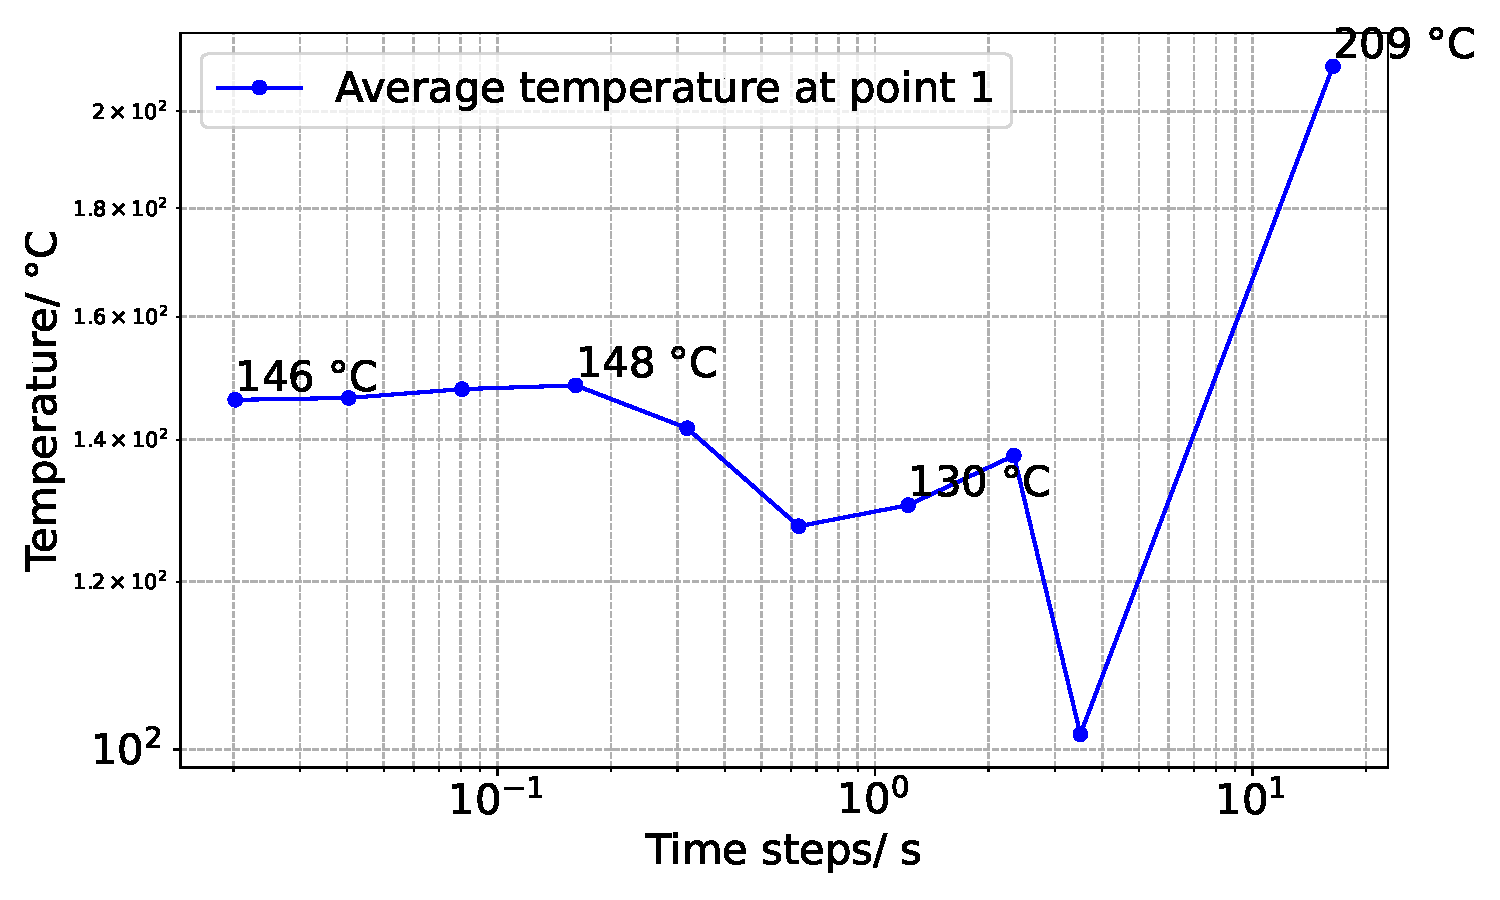
\includegraphics[width=0.8\textwidth]{book/chapters/zhang/graphics/T_ave_vs_dt.pdf}
    \caption{Convergence test, average temperatures of point T1 with time step}
    \label{fig:error_time}
\end{figure}


Figure \ref{fig:error_time} is a comparison of the average temperature of point 1 and times steps. When \(dt\) is above 1 s, the temperature has a large variance. The best value of \(dt\) is 0.16 s (point of 148$^{\circ}\text{C}$ ), which is a balance time step between accuracy and computational time.

\begin{figure}[h]
    \centering
    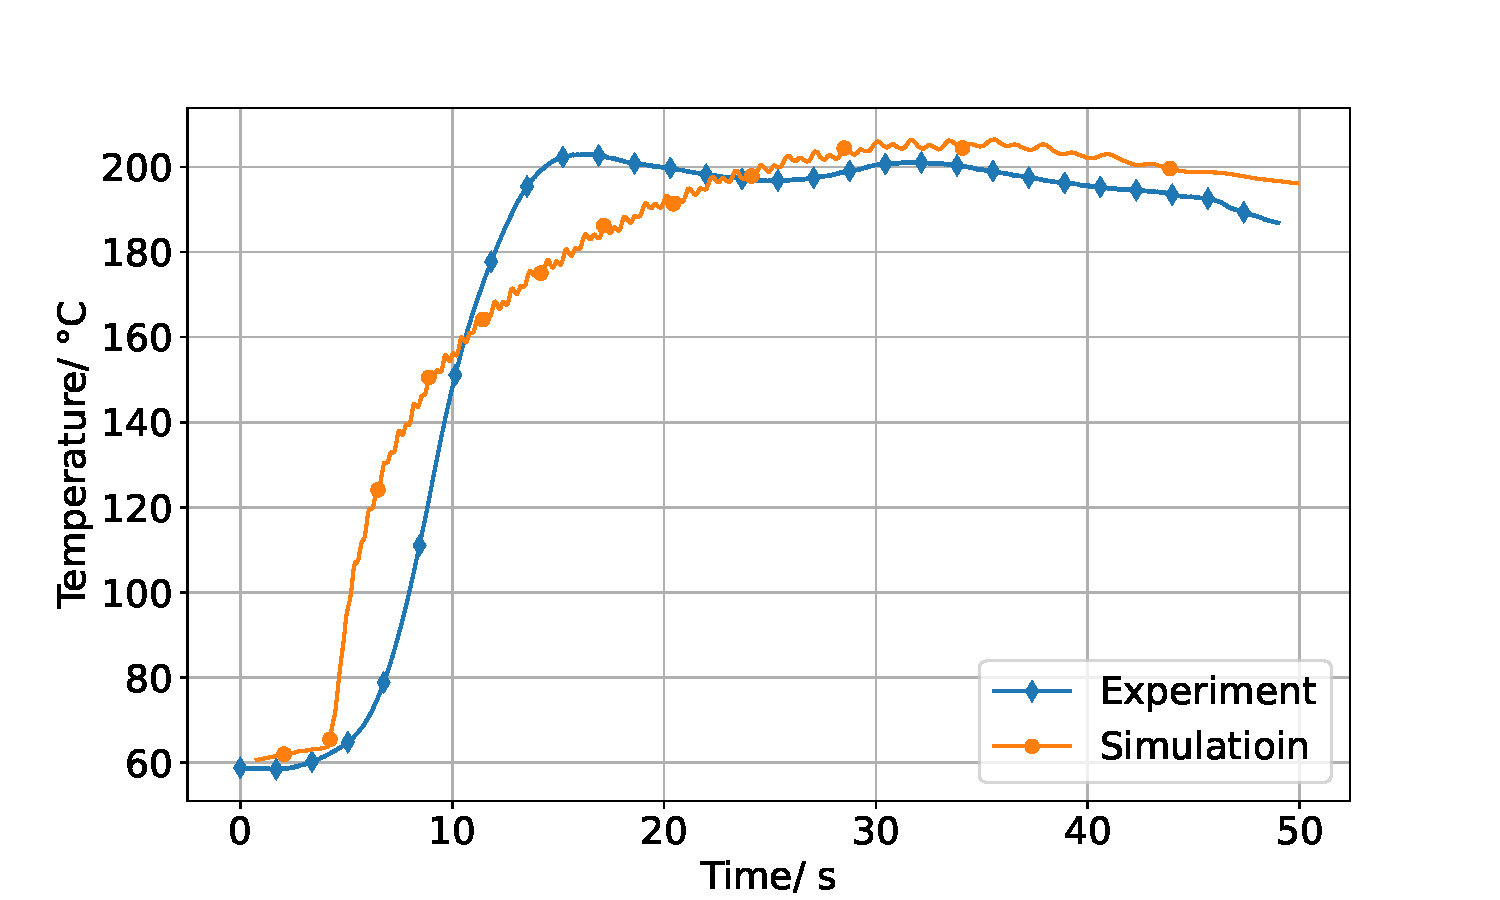
\includegraphics[width=0.8\textwidth]{book/chapters/zhang/graphics/T_sim_exe.pdf}
    \caption{Comparison between simulation time and experimental results}
    \label{fig:experiment}
\end{figure}

Except for mesh and time sensitivities analysis, the simulation results should validated against the experiment. As shown in Figure \ref{fig:experiment}. The general trend of case 1.2 million elements(4.7 million DOFs) and measurement data are the same, so we think the simulation accuracy is acceptable. However, there is still a large space to improve the accuracy. Such as introducing nonlinear material properties. These parameters, such as thermal conductivity, heat capacity, and coefficient of friction are all not constant or linear with temperature, velocity, and pressure. Getting the exact material characteristics is difficult. So better numerical results can benefit from the research of tribology and material engineering. The more detailed experiment parameters, like the loading pressure, would also significantly improve the numerical results since the experiment tests also contain large variances.



\subsection*{Average and maximum temperatures}

This section presents the temperatures of brake discs with different contact areas. The average and the maximum temperatures are presented.
The total contact surface is 200 cm$^2$. The brake pressures from the back of the brake pads are the same, 0.274 MPa, while the different contact areas will affect the contact pressure between the brake pads and discs. 20\%, 50\% and 100\% contact areas are compared. The 20\% contact areas represent the research from Eriksson \cite{eriksson_nature_2002}, and the 100\% contact areas represent most FEM or analytical solutions.

\begin{figure}[h]
    \centering
    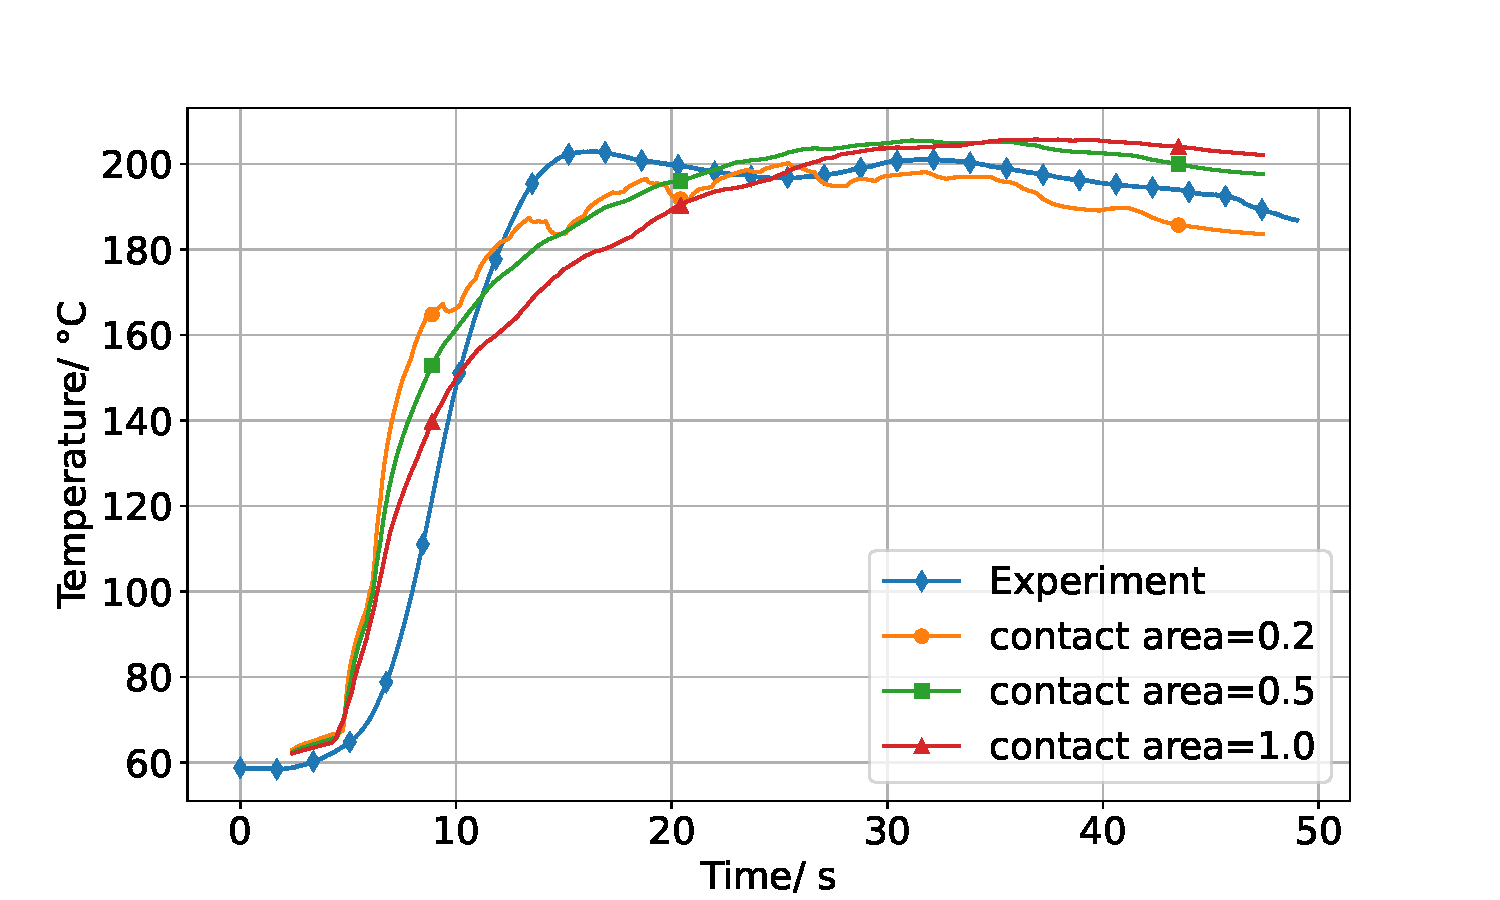
\includegraphics[width=0.8\textwidth]{book/chapters/zhang/graphics/T_ave_dc.pdf}
    \caption{Average temperatures with different contact areas}
    \label{fig:T_ave}
\end{figure}

As shown in Figure \ref{fig:T_ave} is the average temperature for these three cases. The maximum temperature difference is 20 $^{\circ}\text{C}$ between 20\% and 100\% contact areas. The maximum relative difference is 16.6\%. The average temperature is not sensitive to different contact areas since the total heat input is the same, while only heat dissipation is slightly different because the temperature distribution of the brake discs is uneven. Uneven temperature distribution can be proven through the comparison of the maximum temperatures.

\begin{figure}[h]
    \centering
    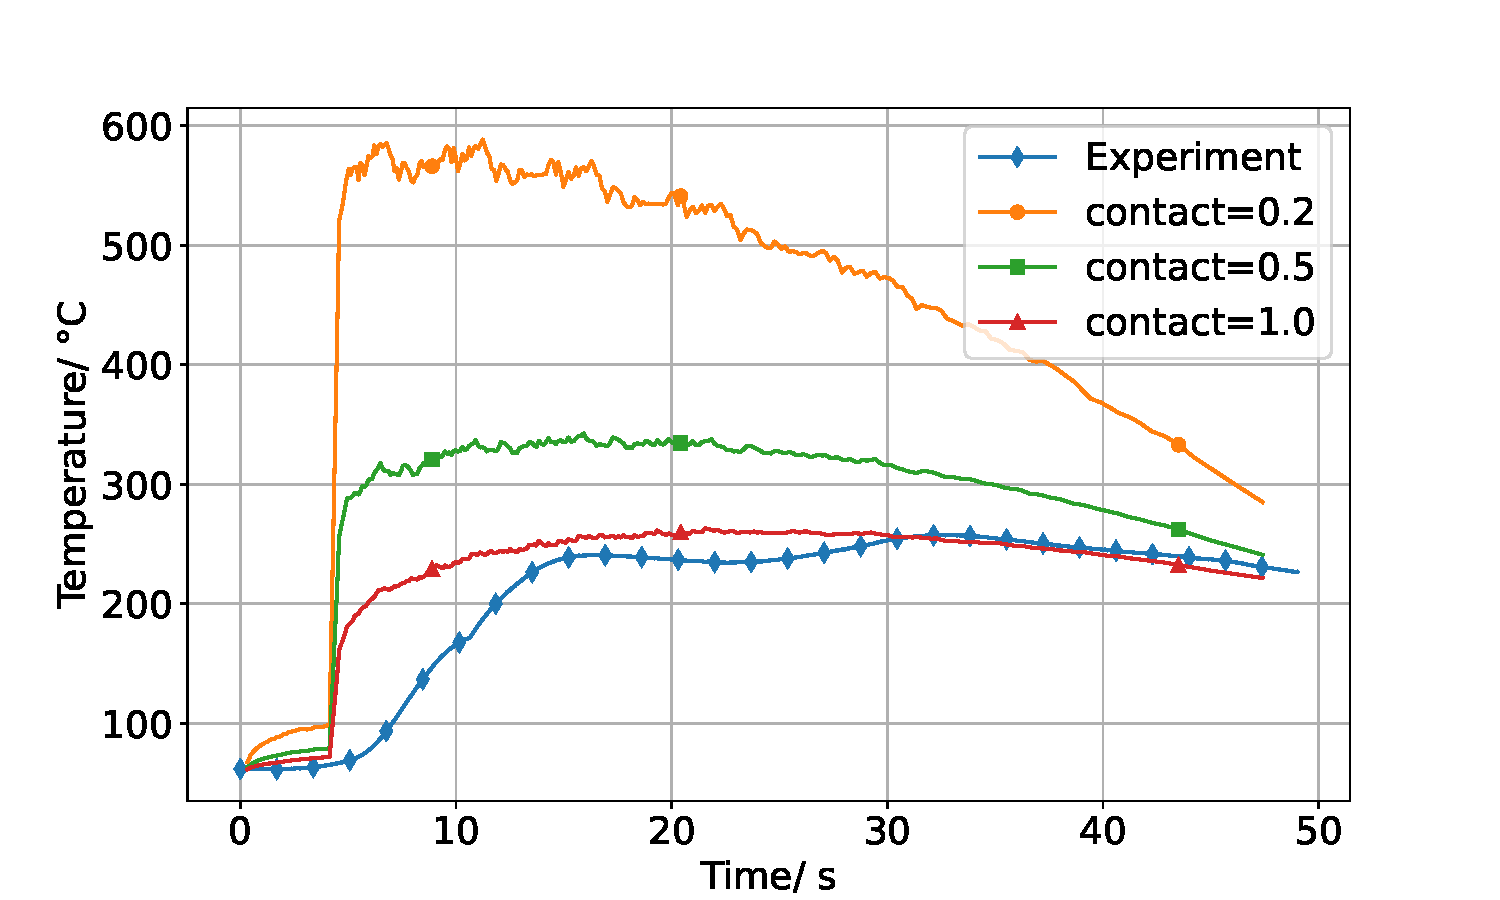
\includegraphics[width=0.8\textwidth]{book/chapters/zhang/graphics/T_max_dc.pdf}
    \caption{The maximum temperatures with different contact areas}
    \label{fig:T_max}
\end{figure}

Figure \ref{fig:T_max} shows the maximum temperature of the brake discs. The maximum temperature difference is more than 300 $^{\circ}\text{C}$, and the relative difference can reach 160\%. Small contact areas induce higher local temperatures since contact pressure is significantly increased and all friction heat is loaded on limited surfaces.

More advanced research can be conducted based on this FEM model, including sensitivity analysis of railway brake disc temperature development. In the future, the following need to be considered to build a more realistic model to investigate different brake designs:

\begin{enumerate}
\item Coupling elastic equations to get deformation details of the brake pads.
\item Considering more nonlinear parameters, like a variable coefficient of friction, and temperature-dependent material properties.
\end{enumerate}


\section*{Conclusion}
This study investigates the influence of contact area on the temperature of railway brake discs. A FEM model in FEniCSx is built and validated. The following conclusions can be drawn:
\begin{enumerate}
\item The contact area does not influence average temperature significantly while a small contact area induces a higher maximum temperature.
\item FEM based research on thermal analysis of brake systems should model real contact areas between brake pads and discs to get an accurate temperature distribution.
\end{enumerate}


\begin{acknowledgement}
This work is sponsored by the KTH Railway Group, China Scholarship Council and CRRC ZELC. Thanks to the experimental support of Fei Gao, Junying Yang at Dalian Jiaotong University. The help of Jørgen S. Dokken from the FEniCSx community and Jing Gong from Kungliga Tekniska Högskolans PDC support are especially acknowledged. Thanks to the National Academic Infrastructure for Supercomputing in Sweden for providing computer resources.        
\end{acknowledgement}

\bibliographystyle{spbasic}
% Write the full path of your bibfile relative to book.tex

\bibliography{chapters/zhang/bibliography.bib}



% Write the full path to the location of the graphics relative to book.tex
\graphicspath{{chapters/zhang/graphics/}}


\title{Thermal analysis of brake discs in rail vehicles}
\titlerunning{Thermal analysis}

\author{Yanjun Zhang, Sebastian Stichel and William Liu}
\authorrunning{Yanjun et al.}

\institute{Yanjun Zhang \email{yanjunzh@kth.se} \at KTH Royal Institute of Technology}

\maketitle

\abstract{}
Railway brake discs convert the kinetic energy of rail vehicles to thermal energy to achieve braking. This thermal energy deteriorates braking performance, therefore, it is necessary to conduct thermal analyses of brake discs. In this work, we build a FEM (finite element method) model in FEniCSx to investigate the influence of contact areas between brake pads and discs on the temperature of brake discs. The weak form of the nonlinear heat transfer equation has been derived, which accounts for conduction, convection and radiation. Multiple Neumann boundary conditions are applied. Simulation results are validated with experimental results. With this efficient FEM model, more advanced research related to railway brake discs can be conducted, such as investigating the effect of wear and thermal expansion, or designing a new geometry of the brake pads and discs.

\section*{Introduction}
Rail vehicles are developed towards higher speed and higher axle load, requiring robust mechanical brake systems for running safety. As shown in figure \ref{fig:disc_block}, one of the most important mechanical brake systems is the disc brake, which converts the kinetic energy of the rail vehicle into heat. A high brake disc temperature reduces the coefficient of friction between the brake discs and the brake pads \cite{Saffar2010}, and causes high thermal stress, which, in turn, induces thermal cracks on the brake discs. To avoid these negative impacts, it is necessary to study the temperature distribution of brake discs. Experimental investigation is relatively complex and can not obtain some parameters, while numerical study is an effective way to address this issue.

\begin{figure}[h]
    \centering
    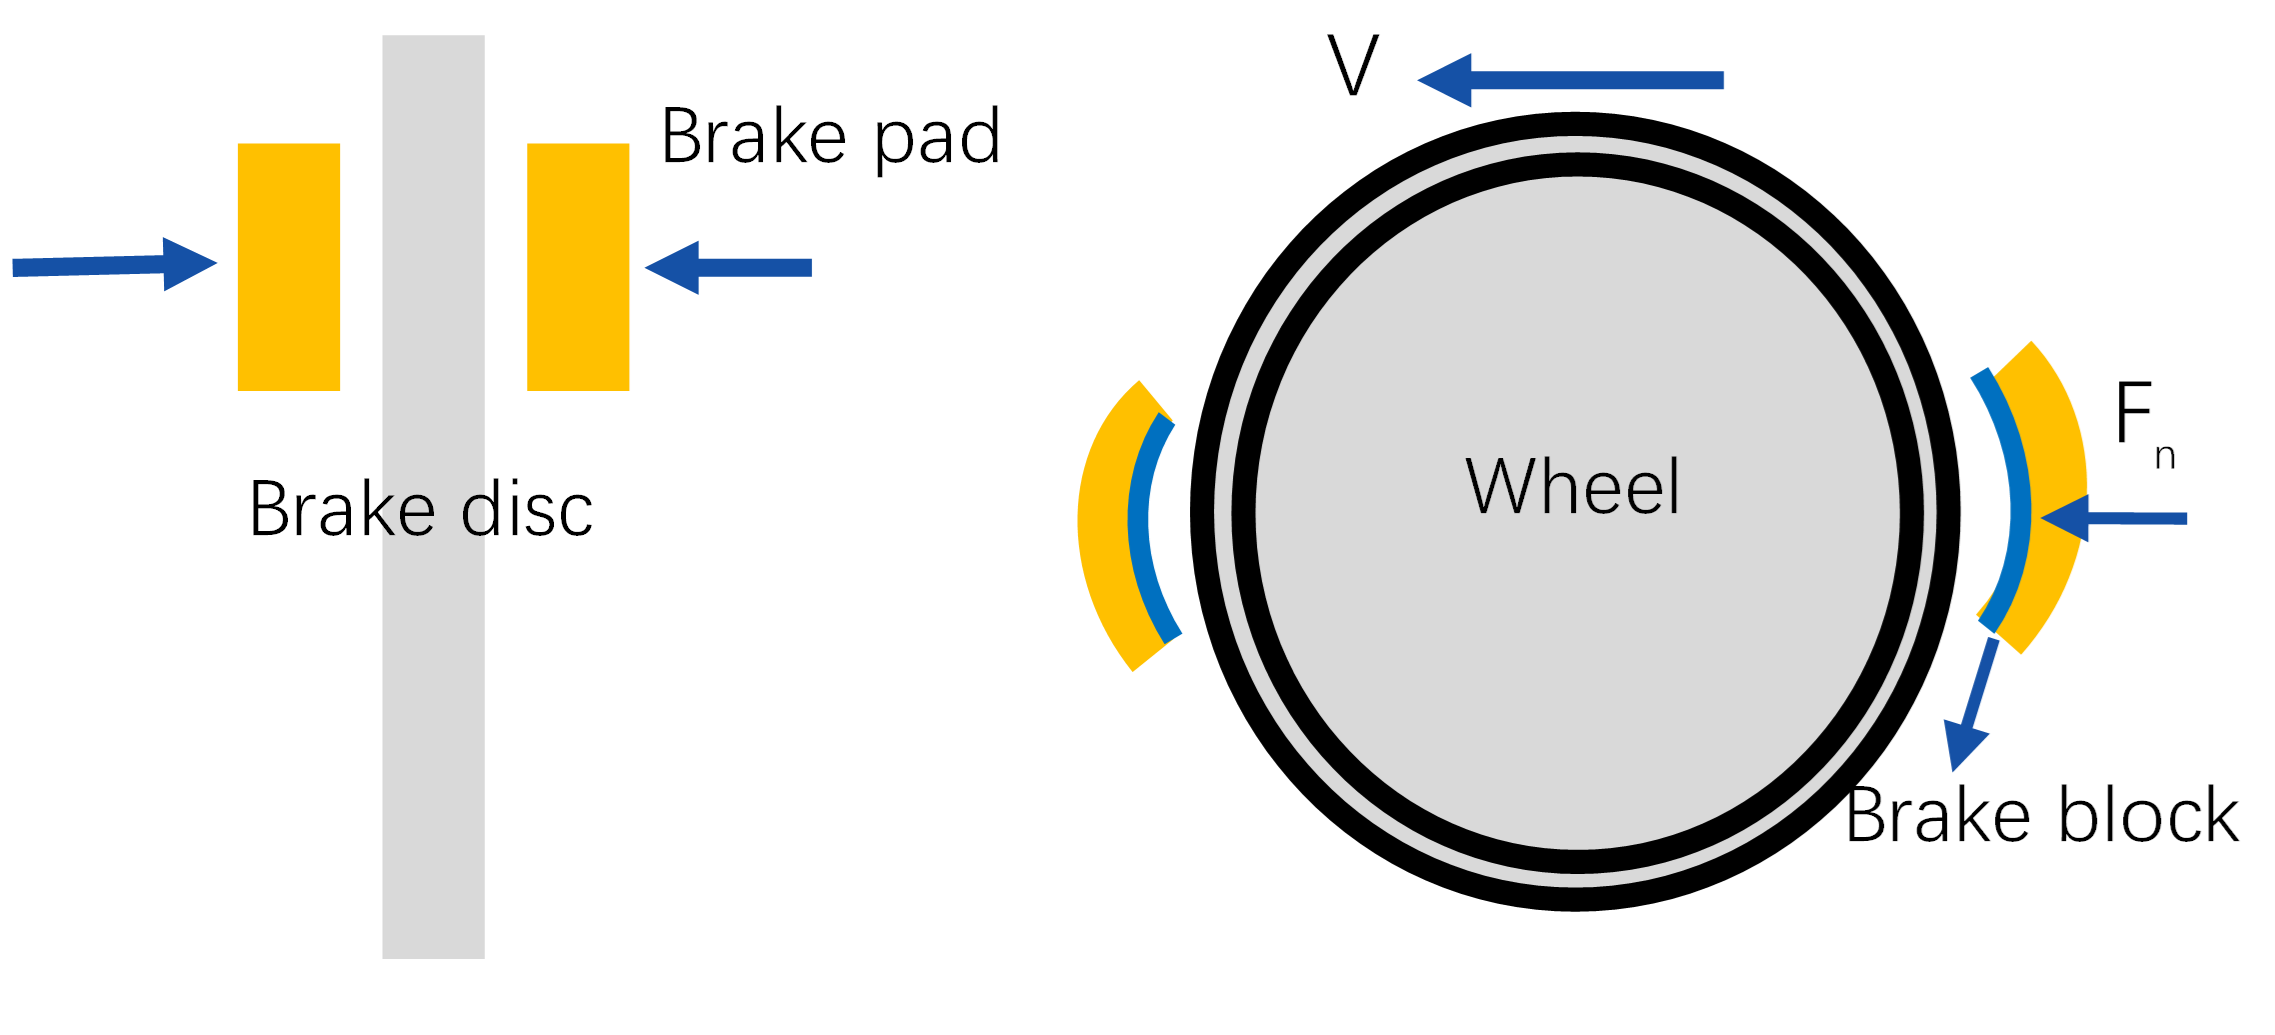
\includegraphics[width=0.65\textwidth]{book/chapters/zhang/graphics/disc_block_brakes.png}
    \caption{Block and disc brakes for rail vehicles}
    \label{fig:disc_block}
\end{figure}

Most thermal analyses of brake discs assume full contact between the brake pads and discs. From tribology studies, the real contact area is around 20\% of the whole brake pad friction surface \cite{eriksson_nature_2002}. Because of thermal expansion and wear of the brake pads, the contact area between the brake pads and discs is always changing. It is difficult to predict the true contact area. However, assuming fixed contact areas, the effect on the temperatures of brake discs can be investigated. This research aims to address the effects of different contact areas on the temperature of the brake discs.



\section*{Methods}

\subsection*{Modelling}
Heat generation and dissipation are two main parts of conducting thermal analysis of railway brake discs. Heat flux is based on friction
\begin{equation}
    q_d = \xi F_f V = \xi P A_d \mu V, 
    \label{heat flux}
\end{equation}

where \( q_d \) is the heat flux in the brake discs (W/m$^2$), \( \xi \) is the heat partition coefficient, \( F_f \) is the friction force (N), \( V \) is the velocity (m/s), \( P \) is the local contact pressure between the brake pads and discs (Pa), \( A_d \) is the friction contact area of the brake pads (m$^2$), and \( \mu \) is the coefficient of friction. Equation \ref{heat flux} is the Neumann boundary condition of Equation \ref{heat equation}, which is the overall heat transfer equation.

The heat flux distribution between the brake pads and discs is vital since it depends on how much heat flows to brake discs, which affects the temperatures and stresses. This coefficient is highly non-linear, affected by material, temperature, and pressure. In this research, this coefficient is simplified to a constant number. The distribution factor is described by \cite{rudolf_limpert_brake_1999}
\begin{equation}
    \xi = \frac{q_p}{q_d + q_p},
\end{equation}
where \( q_p \) is the heat flux in the brake pads (W/m$^2$), and \( q_d \) is the heat flux in the brake discs (W/m$^2$). 

The next step is to build a FEM model of the brake disc. FEM is a method to solve partial differential equations. This method includes the discrete domain, uses an appropriate basis, and rewrites algebraic equations. The heat equation is 
\begin{equation}
    \rho c \frac{\partial T}{\partial t} + \nabla \cdot (- k \nabla T) = f,
    \label{heat equation}
\end{equation}
where \( \rho \) is density, \( c \) is thermal capacity, \( T \) is temperature, \( t \) is time, \( k \) is the overall heat transfer coefficient, and \( f \) is the inner heat source. The time derivative on the right-hand side can be approximated by a difference quotient. Here we use the Euler backward method for consideration of numerical stability. After that, all items are multiplied by a test function \( v \) and integrated by parts. Then according to the divergence theorem, the bilinear form \( a(T,v) \) and linear form \( L(v) \) are

\begin{equation}
    a(T,v) = \frac{\rho c}{\Delta t} \int_\Omega T v dx + \int_\Omega k \nabla T \cdot \nabla v dx + \int_{\partial \Omega} h T v ds + \int_{\partial \Omega} \epsilon \sigma T^4 v ds,
\end{equation}

\begin{equation}
    L_{n+1}(v) = \int_\Omega f^{n+1} v dx 
    + \frac{\rho c}{\Delta t} \int_\Omega  T^{n} v dx 
    -  \int_{\partial \Omega} q v ds
    +  \int_{\partial \Omega} h T_a v ds 
    + \int_{\partial \Omega} \epsilon \sigma T_a^4 v ds,
\end{equation}
where \( \Omega \) is the computation domain, \( \partial \Omega \) is the boundary, \( dx \) is the differential element for integration over the domain, and \( ds \) is the differential element for integration over the boundary, \( h \) is the heat convection coefficient,  \(\Delta t\)\ is the time step, \(n\) is an integer counting time levels. The thermal radiation equation is based on Stefan-Boltzmann Law, where \( \epsilon \) is the emissivity, \( \sigma \) is Stefan-Boltzmann constant, \(T\) is the temperature and \(T^4\) is the temperature to the power of four, \( T_a \) is ambient temperature. For more detailed derivation, please see  \href{https://github.com/Yanjun96/fenicsx/blob/main/derivation_of_heat_transfer.pdf}{derivation of weak form for heat transfer equation}.

The above equation is only for heat transfer, as for brake pad deformation, one needs to solve the elastic equation and here we haven't included here. The main contribution of the elastic deformation calculation is a more accurate contact area between the brake pads and the discs. In this study, we assume that the contact area is known a priori since this research focuses on comparing the influence of different contact areas. The above equations are solved in the FEniCSx platform \cite{baratta_dolfinx_2023,scroggs_construction_2022,alnaes_unified_2014}. All the codes for this paper are in \cite{zhang_thermal_2025}.

The computation domain or mesh is shown in Figure \ref{fig:coarse mesh}. This is a much coarser mesh than the one with 1 million elements used later, with around 43,000 elements. The element type is tetrahedron since when we compared it with hexahedral elements, we found with more tetrahedron elements, the simulation can get the same accuracy with hexahedral elements while tetrahedron has less computation time. Only the brake disc and pad are computation domains. The friction heat, or the Neumann boundary condition is applied on the contact surface, more specifically, only the rubbing elements of the brake pad areas. The rubbing elements are the column structure of the brake pad. Other boundaries include radiation and convection heat transfer, which are also the Neumann boundary conditions without the heat flux input. In each time step, the boundary conditions are redefined since the rotation will change the contact area. In reality, the brake pad should keep still while the brake disc rotates. Here we assumed only the heat flux input areas are rotating: these are the friction heat input areas.

\begin{figure}[h]
    \centering
    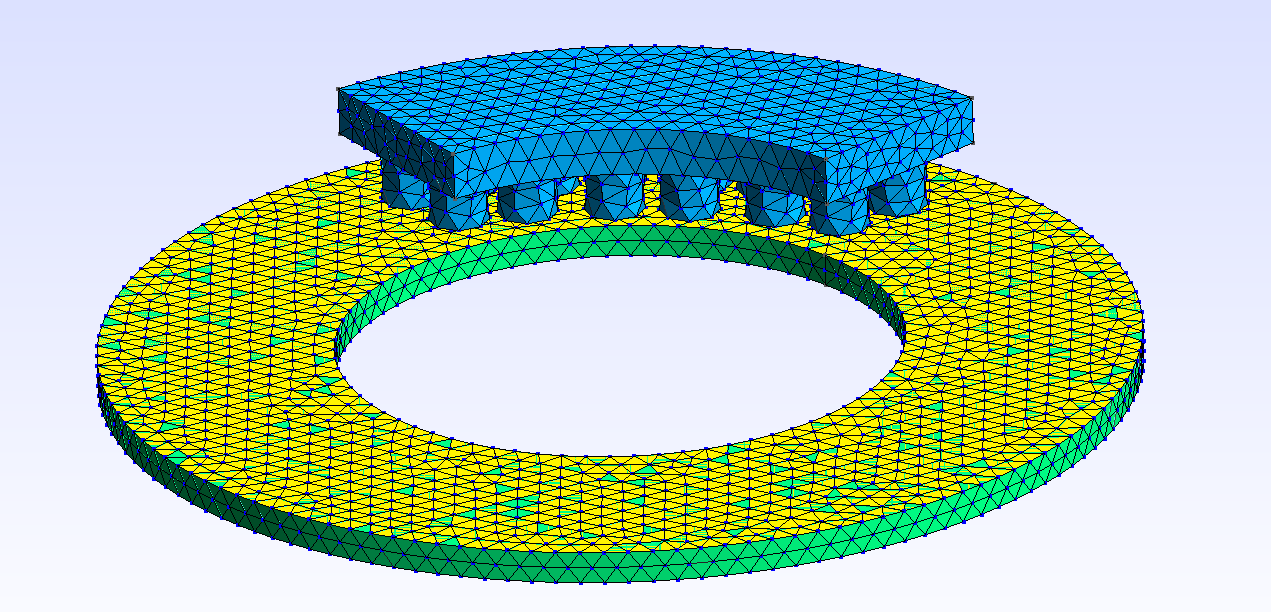
\includegraphics[width=0.9\textwidth]{book/chapters/zhang/graphics/3d surface.png}
    \caption{Computation domain of brake pad and disc, the mesh is much coarser than 1 million case. Friction heat or the Neumann boundary condition is only applied to friction contact areas.}
    \label{fig:coarse mesh}
\end{figure}


\subsection*{Experiment}

The test rig mainly consists of a DC motor, flywheels, brake pad and brake disc, as shown in Figure \ref{fig:test rig}. The maximum motor power is 450 kW, and the maximum motor torque is 4000 Nm. The brake pressure at the reservoir ranges from 0-10 Bar. 
There are in total 6 thermocouples to measure the temperature of the brake disc, which are located under the contact surface. A symmetric model is used in the simulation to save computational effort. The brake lag is the time it takes for the brake pressure to increase from 0\% to 95\% of the target pressure. In the test, the brake lag is 4±0.2 s, which follows the UIC 541-3 standard. Table \ref{tab: operational parameters} shows the operational parameters.

\begin{figure}[h]
    \centering
    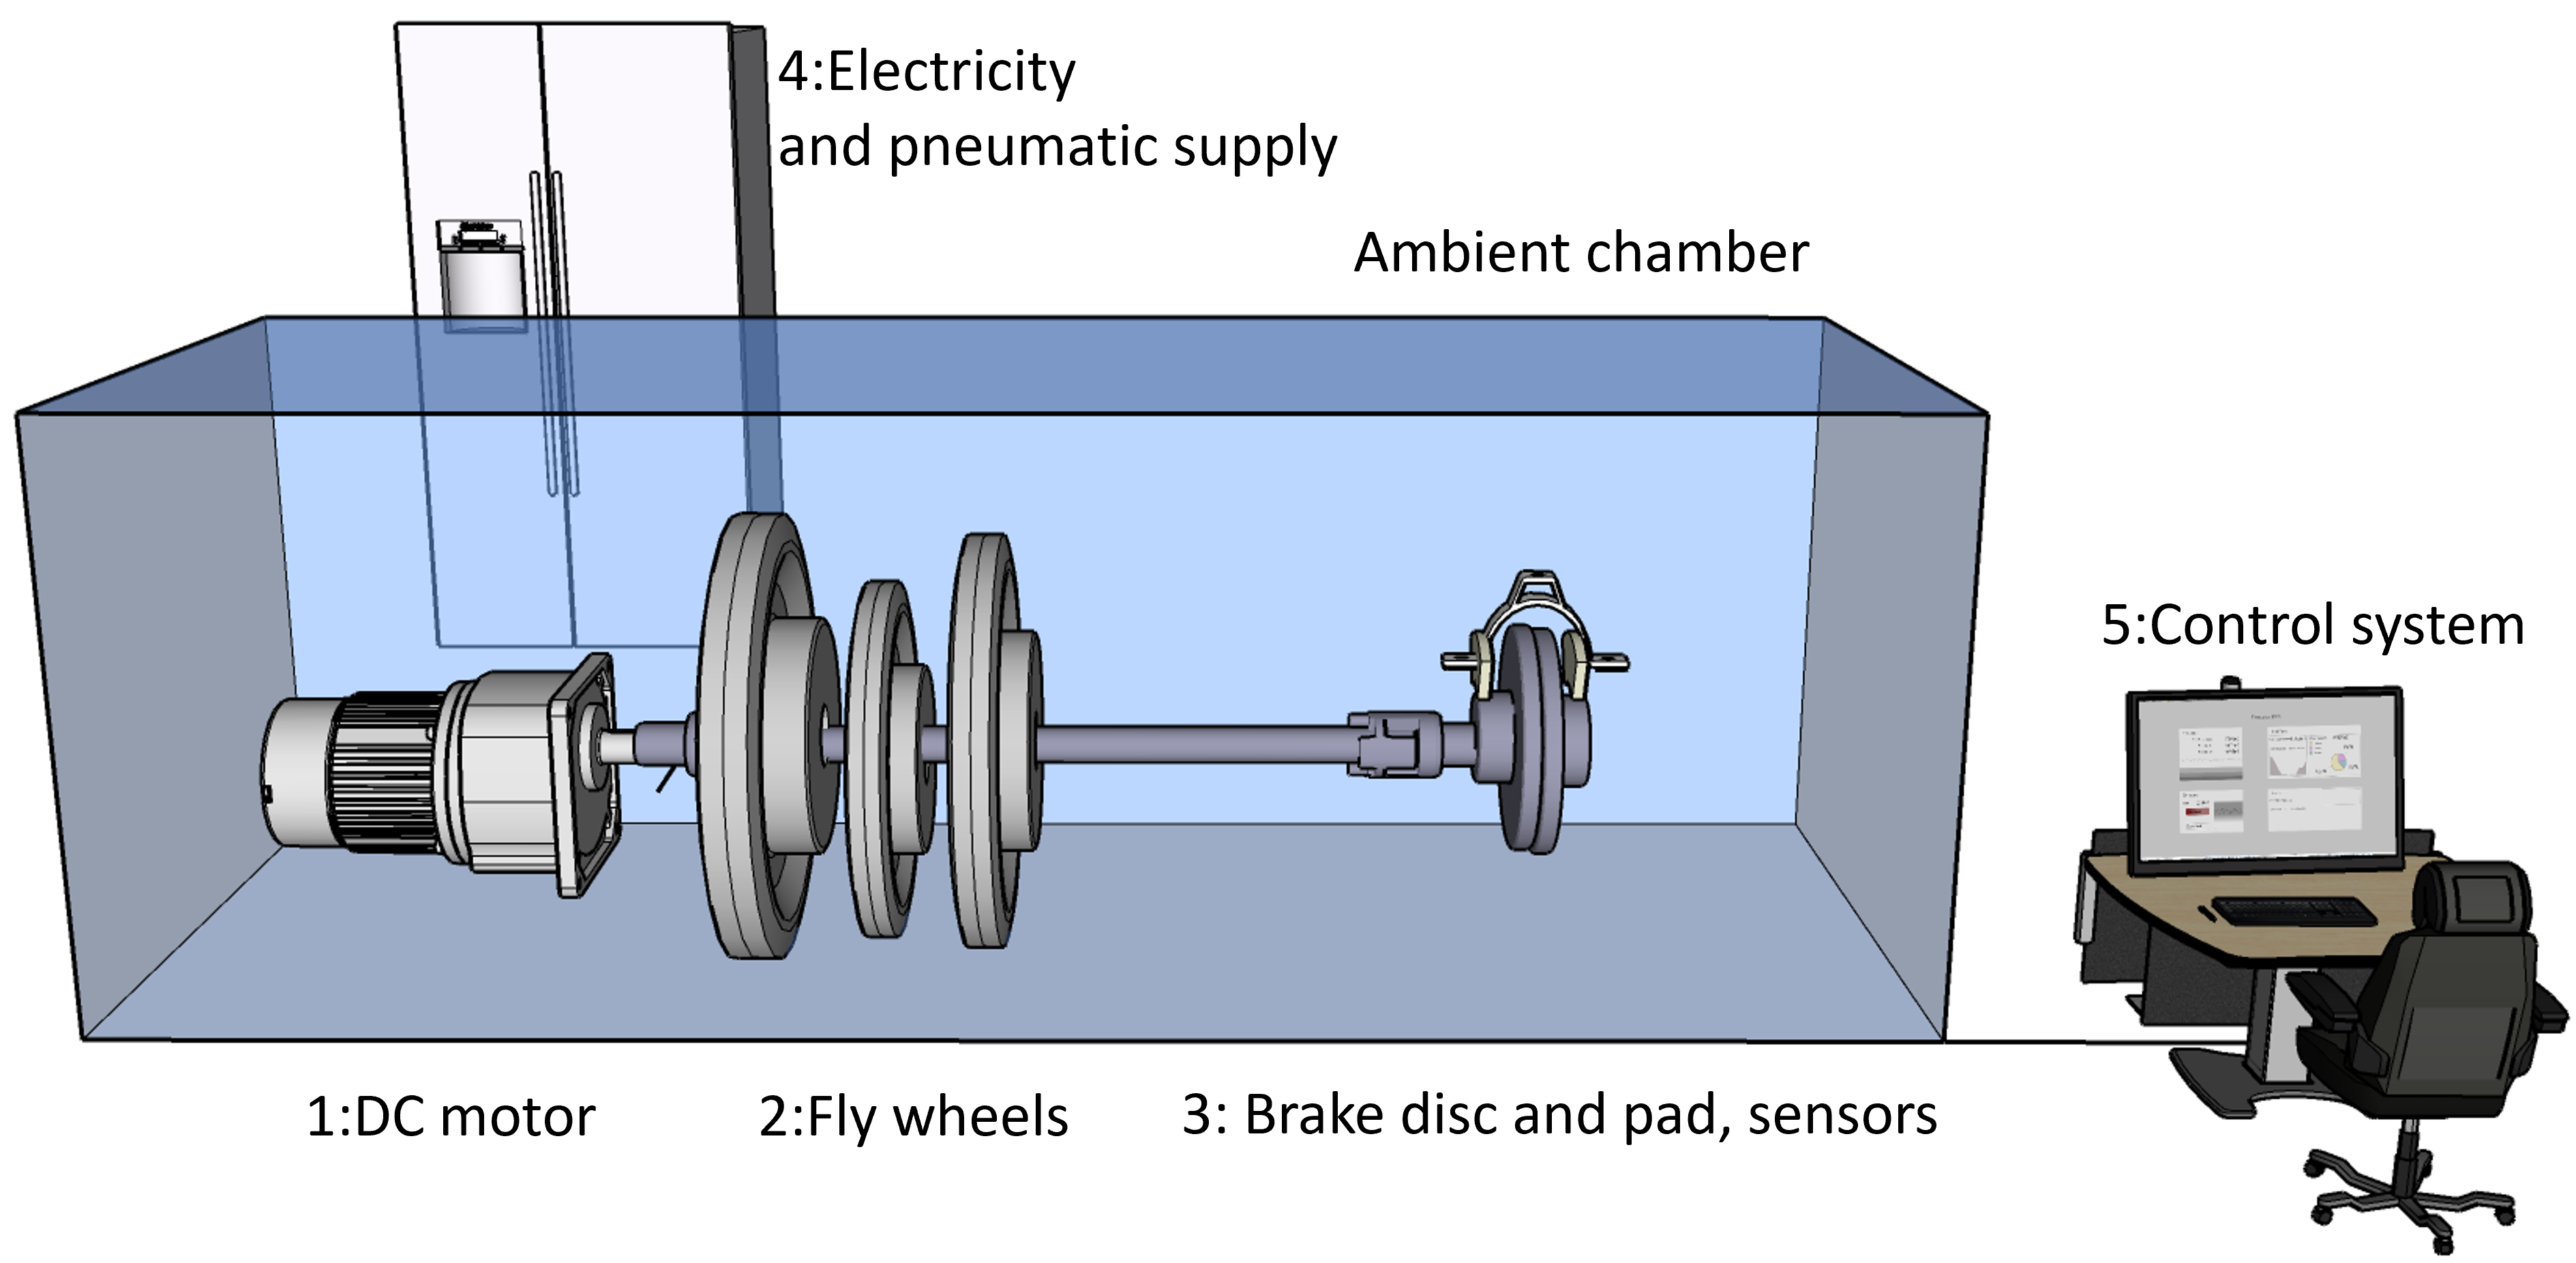
\includegraphics[width=0.85\textwidth]{book/chapters/zhang/graphics/test_rig.png}
    \caption{Full scale railway brake test rig}
    \label{fig:test rig}
\end{figure}

\begin{table}[h]
    \centering
    \begin{tabular}{llll} % 'l' for left-aligned, 'c' for centered
        \toprule
        \textbf{property} & \textbf{quantity} & \textbf{property} & \textbf{quantity}\\ % Header row
        \midrule
        initial velocity (km/h)             & 160       &braking time(s)          & 49 \\
        contact pressure (MPa)              & 0.274      &coefficient of friction  & 0.376 \\
        heat transfer coefficient( W/(m·k)) & 30-125    &heat distributor factor  & 0.88 \\
        brake lag (s)                       & 4         &initial temperature ($^\circ\text{C}$) & 50\\
       
        \bottomrule
    \end{tabular}
    \caption{Brake test parameters}
    \label{tab: operational parameters}
\end{table}

\begin{figure}[h]
    \centering
    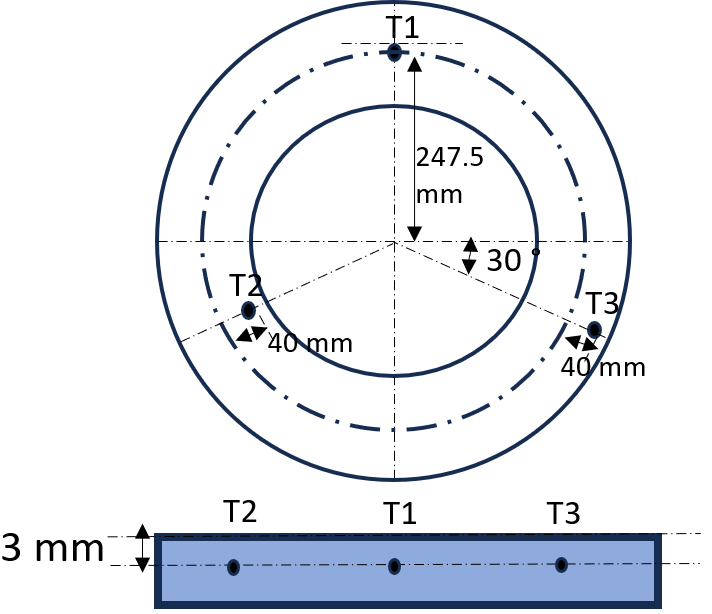
\includegraphics[width=0.45\textwidth]{book/chapters/zhang/graphics/thermo_couples.png}
    \caption{Location of three thermocouples}
    \label{fig:thermocouples}
\end{figure}


\section*{Results and discussion}

\subsection*{Validation}
The first step is mesh sensitivity and time step analysis, where we aim to show that the simulation results converge with finer mesh sizes and smaller time steps. Since no exact solution exist, the average temperature of point T1, as shown in Figure \ref{fig:thermocouples} is used as the convergence parameter.
\begin{figure}
    \centering
    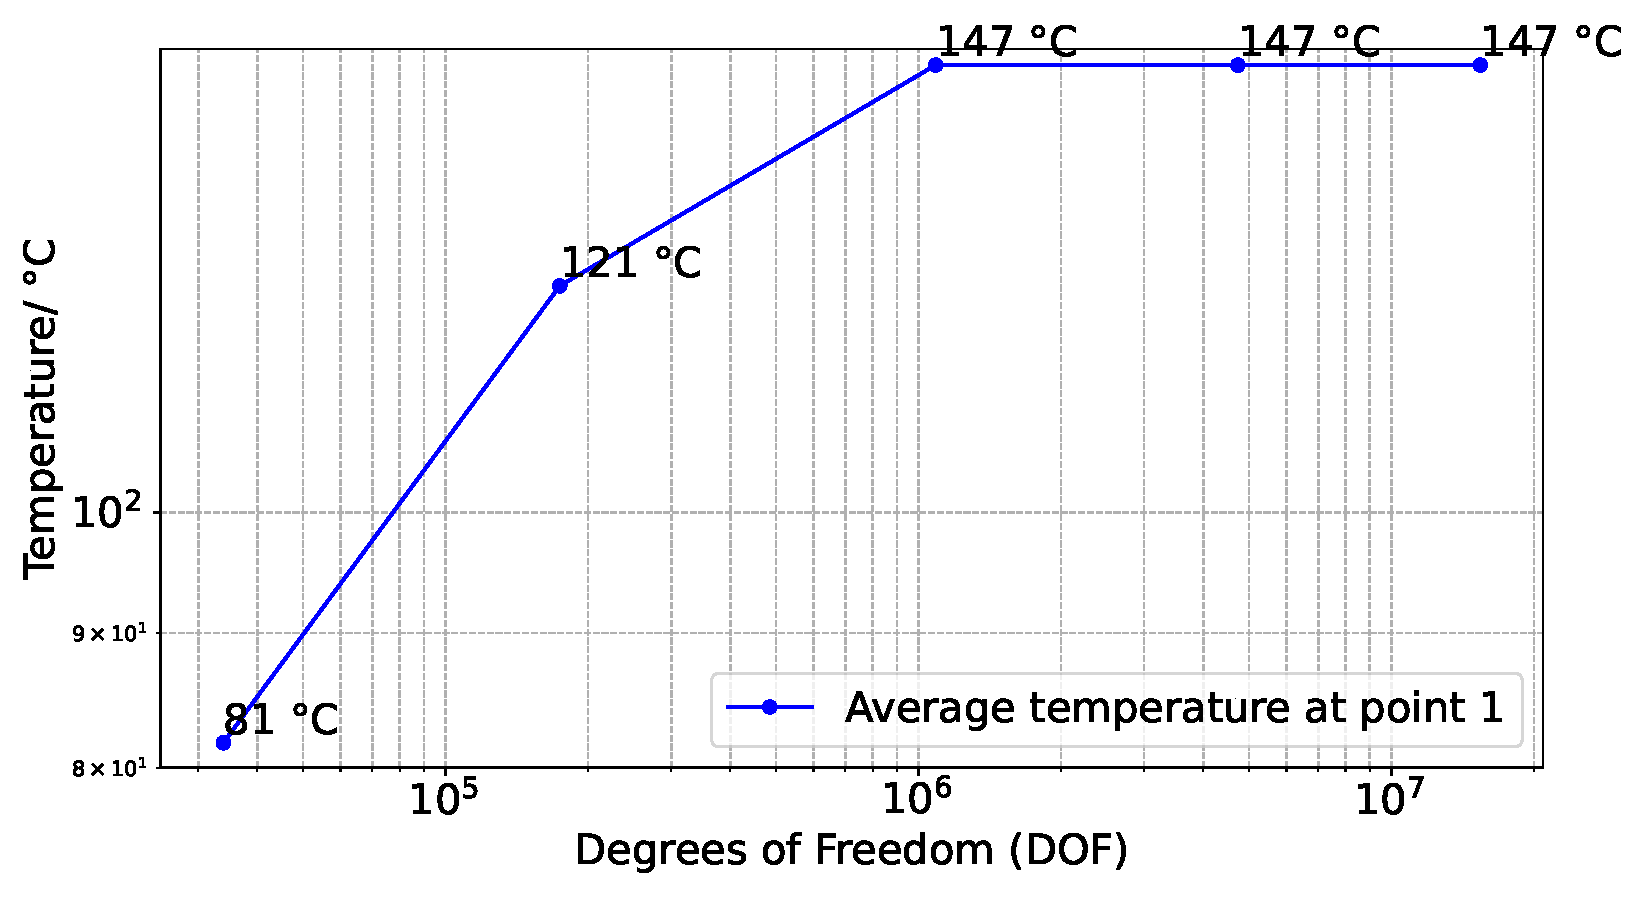
\includegraphics[width=0.8\linewidth]{book/chapters/zhang/graphics/ave_T_vs_dof.pdf}
    \caption{Convergence test, average temperatures of point T1, compared with degrees of freedom (DOFs)}
    \label{fig:error_mesh}
\end{figure}

 As shown in Figure \ref{fig:error_mesh}, the average temperature of point T1 increases with more degrees of freedom until 1 million degrees of freedom (DOFs). Above 1 million, the temperature remains constant.  The above results show that DOFs above 1 million are enough to capture the characteristics of the system. 
\begin{figure}[h]
    \centering
  
    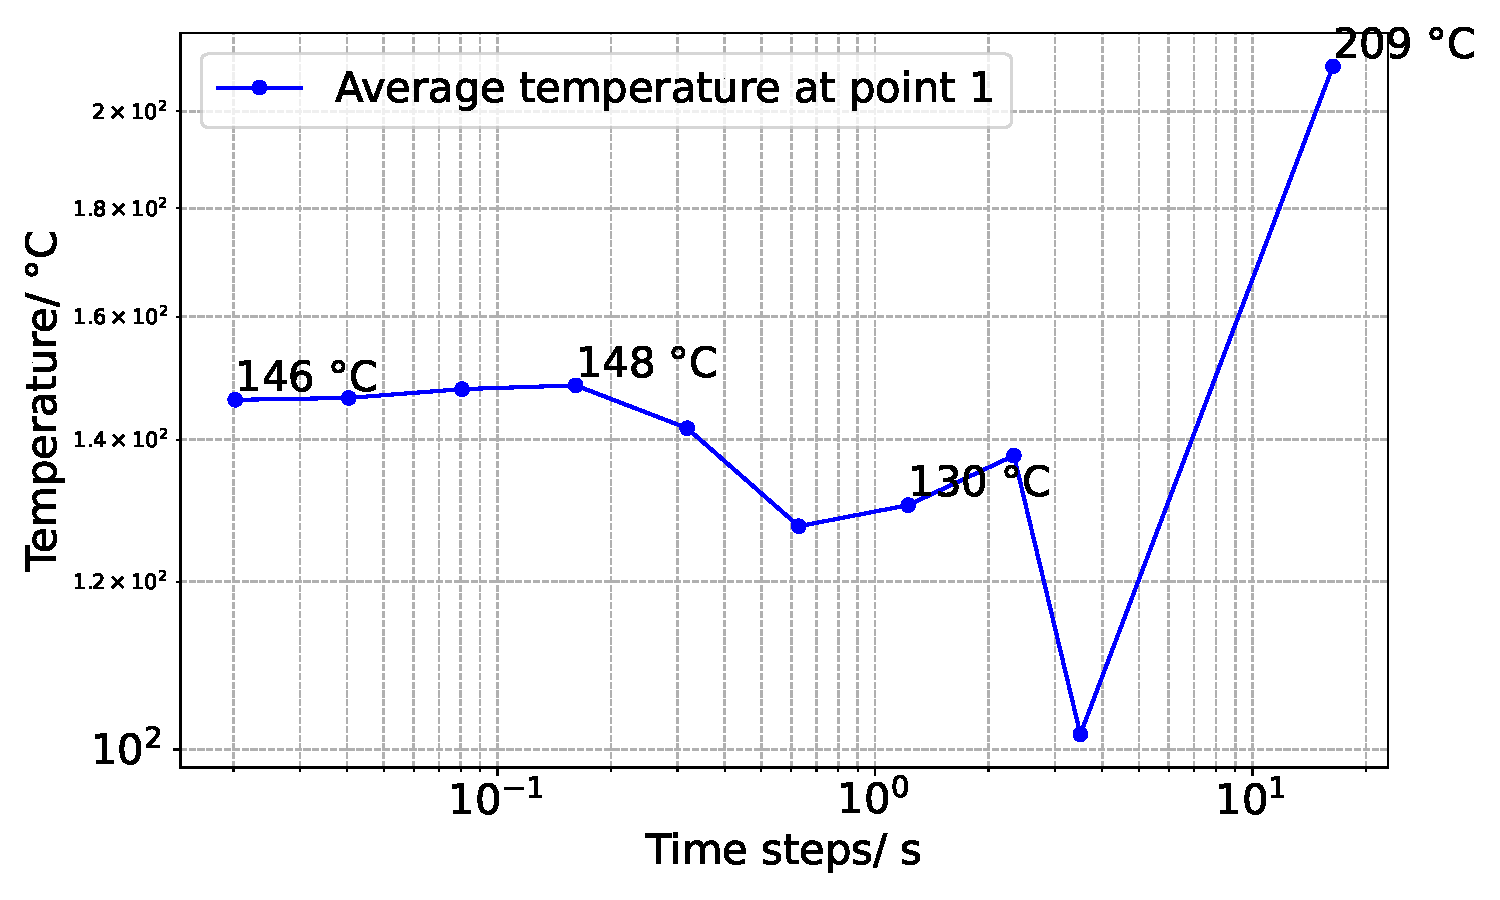
\includegraphics[width=0.8\textwidth]{book/chapters/zhang/graphics/T_ave_vs_dt.pdf}
    \caption{Convergence test, average temperatures of point T1 with time step}
    \label{fig:error_time}
\end{figure}


Figure \ref{fig:error_time} is a comparison of the average temperature of point 1 and times steps. When \(dt\) is above 1 s, the temperature has a large variance. The best value of \(dt\) is 0.16 s (point of 148$^{\circ}\text{C}$ ), which is a balance time step between accuracy and computational time.

\begin{figure}[h]
    \centering
    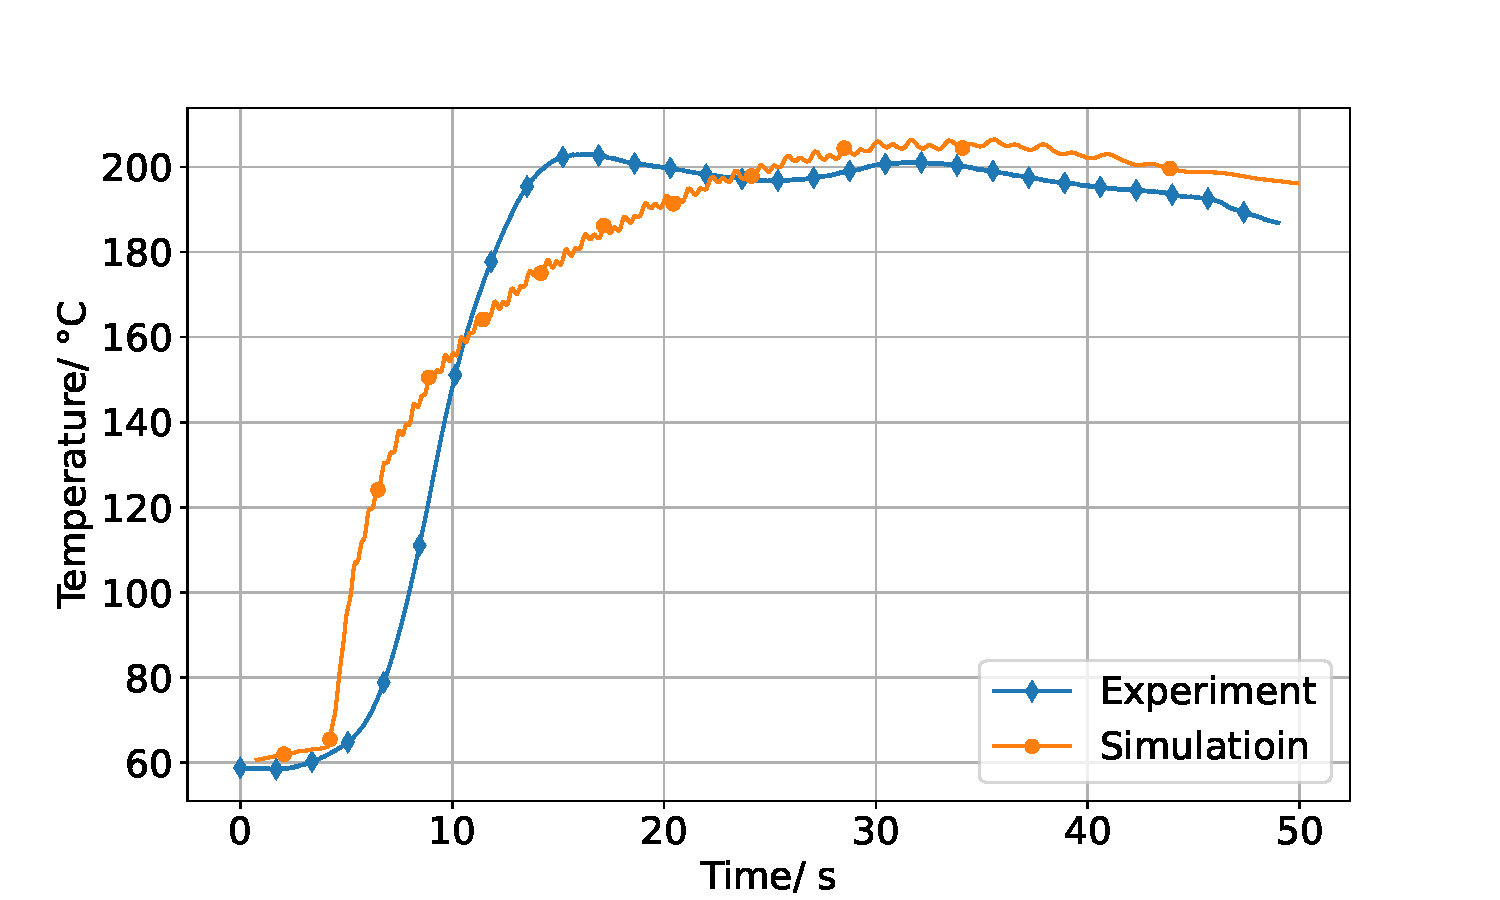
\includegraphics[width=0.8\textwidth]{book/chapters/zhang/graphics/T_sim_exe.pdf}
    \caption{Comparison between simulation time and experimental results}
    \label{fig:experiment}
\end{figure}

Except for mesh and time sensitivities analysis, the simulation results should validated against the experiment. As shown in Figure \ref{fig:experiment}. The general trend of case 1.2 million elements(4.7 million DOFs) and measurement data are the same, so we think the simulation accuracy is acceptable. However, there is still a large space to improve the accuracy. Such as introducing nonlinear material properties. These parameters, such as thermal conductivity, heat capacity, and coefficient of friction are all not constant or linear with temperature, velocity, and pressure. Getting the exact material characteristics is difficult. So better numerical results can benefit from the research of tribology and material engineering. The more detailed experiment parameters, like the loading pressure, would also significantly improve the numerical results since the experiment tests also contain large variances.



\subsection*{Average and maximum temperatures}

This section presents the temperatures of brake discs with different contact areas. The average and the maximum temperatures are presented.
The total contact surface is 200 cm$^2$. The brake pressures from the back of the brake pads are the same, 0.274 MPa, while the different contact areas will affect the contact pressure between the brake pads and discs. 20\%, 50\% and 100\% contact areas are compared. The 20\% contact areas represent the research from Eriksson \cite{eriksson_nature_2002}, and the 100\% contact areas represent most FEM or analytical solutions.

\begin{figure}[h]
    \centering
    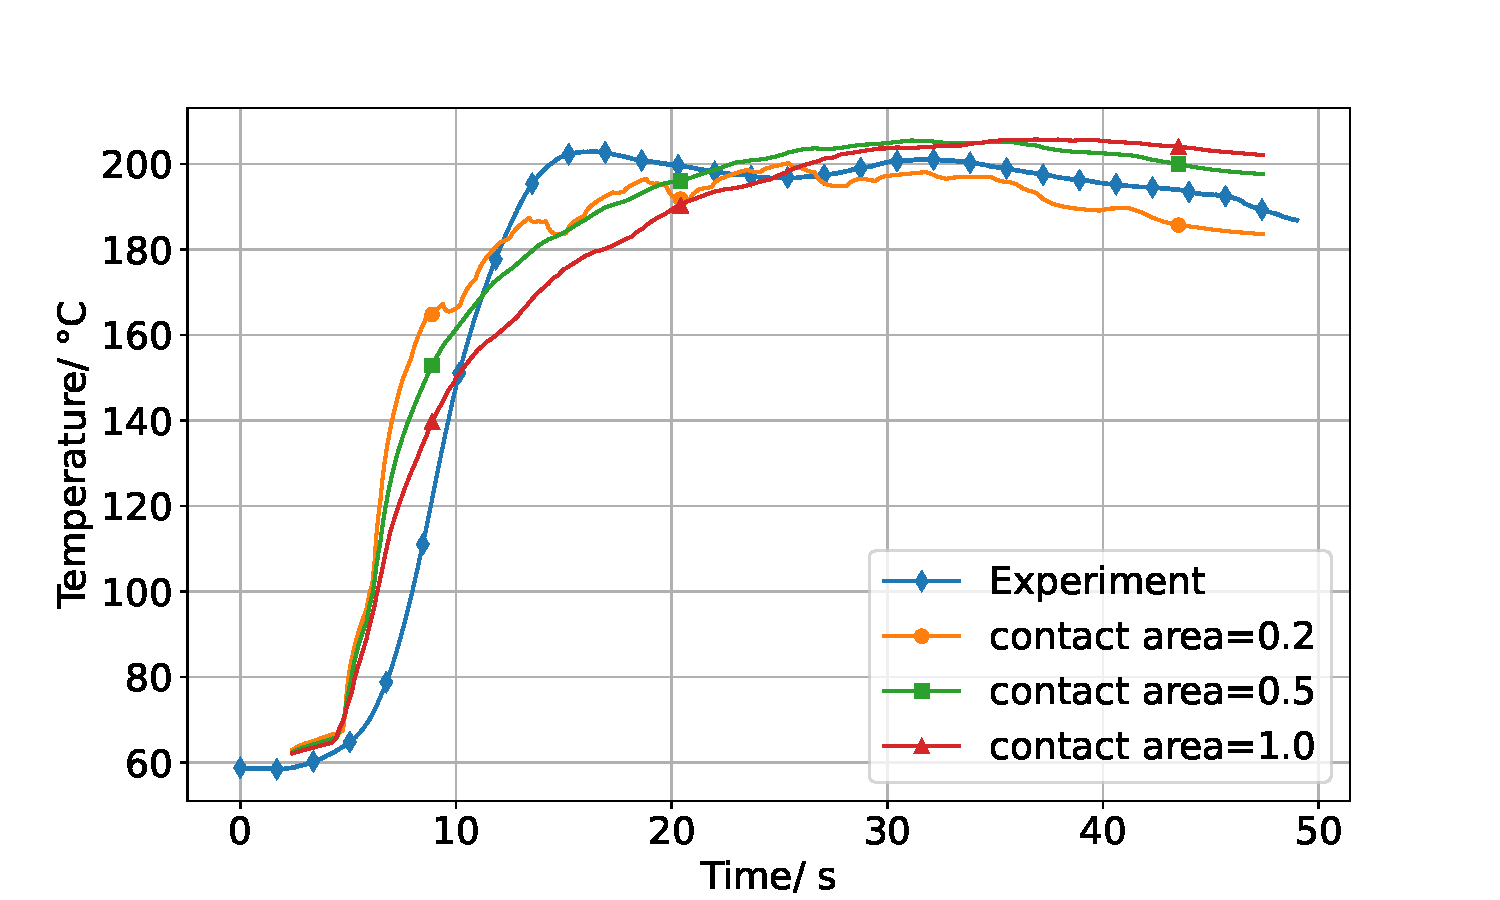
\includegraphics[width=0.8\textwidth]{book/chapters/zhang/graphics/T_ave_dc.pdf}
    \caption{Average temperatures with different contact areas}
    \label{fig:T_ave}
\end{figure}

As shown in Figure \ref{fig:T_ave} is the average temperature for these three cases. The maximum temperature difference is 20 $^{\circ}\text{C}$ between 20\% and 100\% contact areas. The maximum relative difference is 16.6\%. The average temperature is not sensitive to different contact areas since the total heat input is the same, while only heat dissipation is slightly different because the temperature distribution of the brake discs is uneven. Uneven temperature distribution can be proven through the comparison of the maximum temperatures.

\begin{figure}[h]
    \centering
    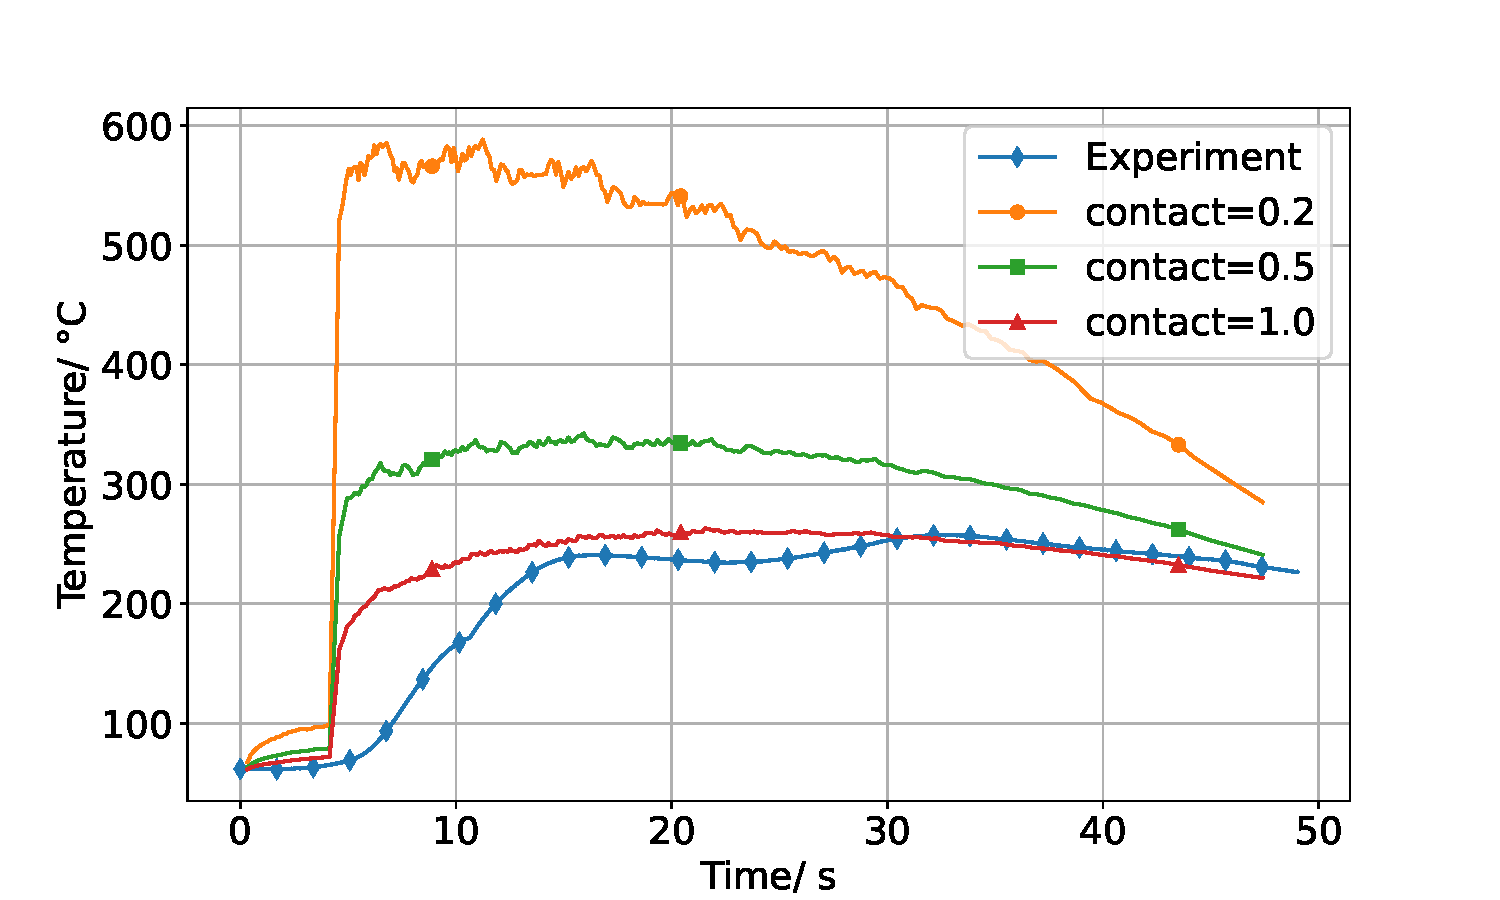
\includegraphics[width=0.8\textwidth]{book/chapters/zhang/graphics/T_max_dc.pdf}
    \caption{The maximum temperatures with different contact areas}
    \label{fig:T_max}
\end{figure}

Figure \ref{fig:T_max} shows the maximum temperature of the brake discs. The maximum temperature difference is more than 300 $^{\circ}\text{C}$, and the relative difference can reach 160\%. Small contact areas induce higher local temperatures since contact pressure is significantly increased and all friction heat is loaded on limited surfaces.

More advanced research can be conducted based on this FEM model, including sensitivity analysis of railway brake disc temperature development. In the future, the following need to be considered to build a more realistic model to investigate different brake designs:

\begin{enumerate}
\item Coupling elastic equations to get deformation details of the brake pads.
\item Considering more nonlinear parameters, like a variable coefficient of friction, and temperature-dependent material properties.
\end{enumerate}


\section*{Conclusion}
This study investigates the influence of contact area on the temperature of railway brake discs. A FEM model in FEniCSx is built and validated. The following conclusions can be drawn:
\begin{enumerate}
\item The contact area does not influence average temperature significantly while a small contact area induces a higher maximum temperature.
\item FEM based research on thermal analysis of brake systems should model real contact areas between brake pads and discs to get an accurate temperature distribution.
\end{enumerate}


\begin{acknowledgement}
This work is sponsored by the KTH Railway Group, China Scholarship Council and CRRC ZELC. Thanks to the experimental support of Fei Gao, Junying Yang at Dalian Jiaotong University. The help of Jørgen S. Dokken from the FEniCSx community and Jing Gong from Kungliga Tekniska Högskolans PDC support are especially acknowledged. Thanks to the National Academic Infrastructure for Supercomputing in Sweden for providing computer resources.        
\end{acknowledgement}

\bibliographystyle{spbasic}
% Write the full path of your bibfile relative to book.tex

\bibliography{chapters/zhang/bibliography.bib}



% Write the full path to the location of the graphics relative to book.tex
\graphicspath{{chapters/zhang/graphics/}}


\title{Thermal analysis of brake discs in rail vehicles}
\titlerunning{Thermal analysis}

\author{Yanjun Zhang, Sebastian Stichel and William Liu}
\authorrunning{Yanjun et al.}

\institute{Yanjun Zhang \email{yanjunzh@kth.se} \at KTH Royal Institute of Technology}

\maketitle

\abstract{}
Railway brake discs convert the kinetic energy of rail vehicles to thermal energy to achieve braking. This thermal energy deteriorates braking performance, therefore, it is necessary to conduct thermal analyses of brake discs. In this work, we build a FEM (finite element method) model in FEniCSx to investigate the influence of contact areas between brake pads and discs on the temperature of brake discs. The weak form of the nonlinear heat transfer equation has been derived, which accounts for conduction, convection and radiation. Multiple Neumann boundary conditions are applied. Simulation results are validated with experimental results. With this efficient FEM model, more advanced research related to railway brake discs can be conducted, such as investigating the effect of wear and thermal expansion, or designing a new geometry of the brake pads and discs.

\section*{Introduction}
Rail vehicles are developed towards higher speed and higher axle load, requiring robust mechanical brake systems for running safety. As shown in figure \ref{fig:disc_block}, one of the most important mechanical brake systems is the disc brake, which converts the kinetic energy of the rail vehicle into heat. A high brake disc temperature reduces the coefficient of friction between the brake discs and the brake pads \cite{Saffar2010}, and causes high thermal stress, which, in turn, induces thermal cracks on the brake discs. To avoid these negative impacts, it is necessary to study the temperature distribution of brake discs. Experimental investigation is relatively complex and can not obtain some parameters, while numerical study is an effective way to address this issue.

\begin{figure}[h]
    \centering
    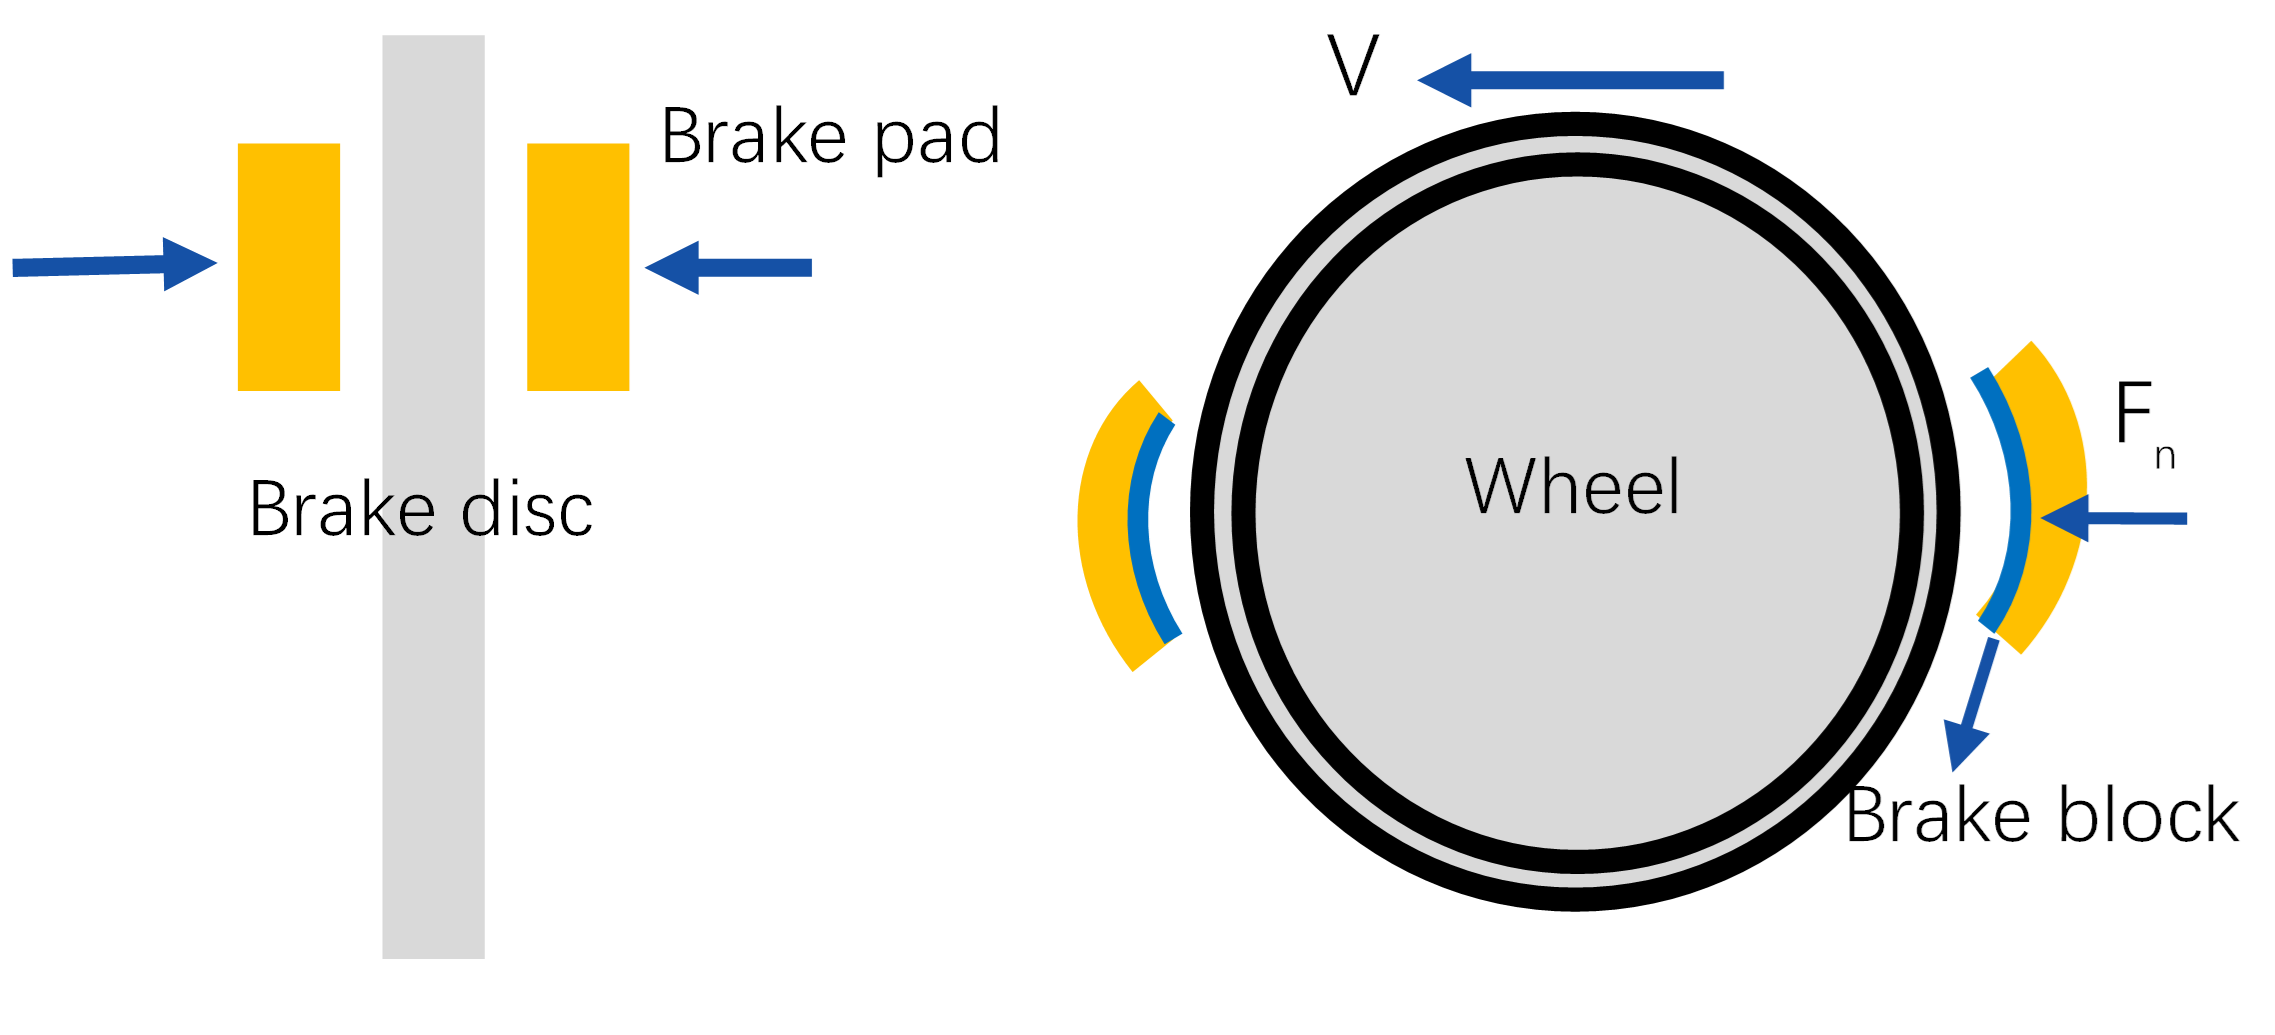
\includegraphics[width=0.65\textwidth]{book/chapters/zhang/graphics/disc_block_brakes.png}
    \caption{Block and disc brakes for rail vehicles}
    \label{fig:disc_block}
\end{figure}

Most thermal analyses of brake discs assume full contact between the brake pads and discs. From tribology studies, the real contact area is around 20\% of the whole brake pad friction surface \cite{eriksson_nature_2002}. Because of thermal expansion and wear of the brake pads, the contact area between the brake pads and discs is always changing. It is difficult to predict the true contact area. However, assuming fixed contact areas, the effect on the temperatures of brake discs can be investigated. This research aims to address the effects of different contact areas on the temperature of the brake discs.



\section*{Methods}

\subsection*{Modelling}
Heat generation and dissipation are two main parts of conducting thermal analysis of railway brake discs. Heat flux is based on friction
\begin{equation}
    q_d = \xi F_f V = \xi P A_d \mu V, 
    \label{heat flux}
\end{equation}

where \( q_d \) is the heat flux in the brake discs (W/m$^2$), \( \xi \) is the heat partition coefficient, \( F_f \) is the friction force (N), \( V \) is the velocity (m/s), \( P \) is the local contact pressure between the brake pads and discs (Pa), \( A_d \) is the friction contact area of the brake pads (m$^2$), and \( \mu \) is the coefficient of friction. Equation \ref{heat flux} is the Neumann boundary condition of Equation \ref{heat equation}, which is the overall heat transfer equation.

The heat flux distribution between the brake pads and discs is vital since it depends on how much heat flows to brake discs, which affects the temperatures and stresses. This coefficient is highly non-linear, affected by material, temperature, and pressure. In this research, this coefficient is simplified to a constant number. The distribution factor is described by \cite{rudolf_limpert_brake_1999}
\begin{equation}
    \xi = \frac{q_p}{q_d + q_p},
\end{equation}
where \( q_p \) is the heat flux in the brake pads (W/m$^2$), and \( q_d \) is the heat flux in the brake discs (W/m$^2$). 

The next step is to build a FEM model of the brake disc. FEM is a method to solve partial differential equations. This method includes the discrete domain, uses an appropriate basis, and rewrites algebraic equations. The heat equation is 
\begin{equation}
    \rho c \frac{\partial T}{\partial t} + \nabla \cdot (- k \nabla T) = f,
    \label{heat equation}
\end{equation}
where \( \rho \) is density, \( c \) is thermal capacity, \( T \) is temperature, \( t \) is time, \( k \) is the overall heat transfer coefficient, and \( f \) is the inner heat source. The time derivative on the right-hand side can be approximated by a difference quotient. Here we use the Euler backward method for consideration of numerical stability. After that, all items are multiplied by a test function \( v \) and integrated by parts. Then according to the divergence theorem, the bilinear form \( a(T,v) \) and linear form \( L(v) \) are

\begin{equation}
    a(T,v) = \frac{\rho c}{\Delta t} \int_\Omega T v dx + \int_\Omega k \nabla T \cdot \nabla v dx + \int_{\partial \Omega} h T v ds + \int_{\partial \Omega} \epsilon \sigma T^4 v ds,
\end{equation}

\begin{equation}
    L_{n+1}(v) = \int_\Omega f^{n+1} v dx 
    + \frac{\rho c}{\Delta t} \int_\Omega  T^{n} v dx 
    -  \int_{\partial \Omega} q v ds
    +  \int_{\partial \Omega} h T_a v ds 
    + \int_{\partial \Omega} \epsilon \sigma T_a^4 v ds,
\end{equation}
where \( \Omega \) is the computation domain, \( \partial \Omega \) is the boundary, \( dx \) is the differential element for integration over the domain, and \( ds \) is the differential element for integration over the boundary, \( h \) is the heat convection coefficient,  \(\Delta t\)\ is the time step, \(n\) is an integer counting time levels. The thermal radiation equation is based on Stefan-Boltzmann Law, where \( \epsilon \) is the emissivity, \( \sigma \) is Stefan-Boltzmann constant, \(T\) is the temperature and \(T^4\) is the temperature to the power of four, \( T_a \) is ambient temperature. For more detailed derivation, please see  \href{https://github.com/Yanjun96/fenicsx/blob/main/derivation_of_heat_transfer.pdf}{derivation of weak form for heat transfer equation}.

The above equation is only for heat transfer, as for brake pad deformation, one needs to solve the elastic equation and here we haven't included here. The main contribution of the elastic deformation calculation is a more accurate contact area between the brake pads and the discs. In this study, we assume that the contact area is known a priori since this research focuses on comparing the influence of different contact areas. The above equations are solved in the FEniCSx platform \cite{baratta_dolfinx_2023,scroggs_construction_2022,alnaes_unified_2014}. All the codes for this paper are in \cite{zhang_thermal_2025}.

The computation domain or mesh is shown in Figure \ref{fig:coarse mesh}. This is a much coarser mesh than the one with 1 million elements used later, with around 43,000 elements. The element type is tetrahedron since when we compared it with hexahedral elements, we found with more tetrahedron elements, the simulation can get the same accuracy with hexahedral elements while tetrahedron has less computation time. Only the brake disc and pad are computation domains. The friction heat, or the Neumann boundary condition is applied on the contact surface, more specifically, only the rubbing elements of the brake pad areas. The rubbing elements are the column structure of the brake pad. Other boundaries include radiation and convection heat transfer, which are also the Neumann boundary conditions without the heat flux input. In each time step, the boundary conditions are redefined since the rotation will change the contact area. In reality, the brake pad should keep still while the brake disc rotates. Here we assumed only the heat flux input areas are rotating: these are the friction heat input areas.

\begin{figure}[h]
    \centering
    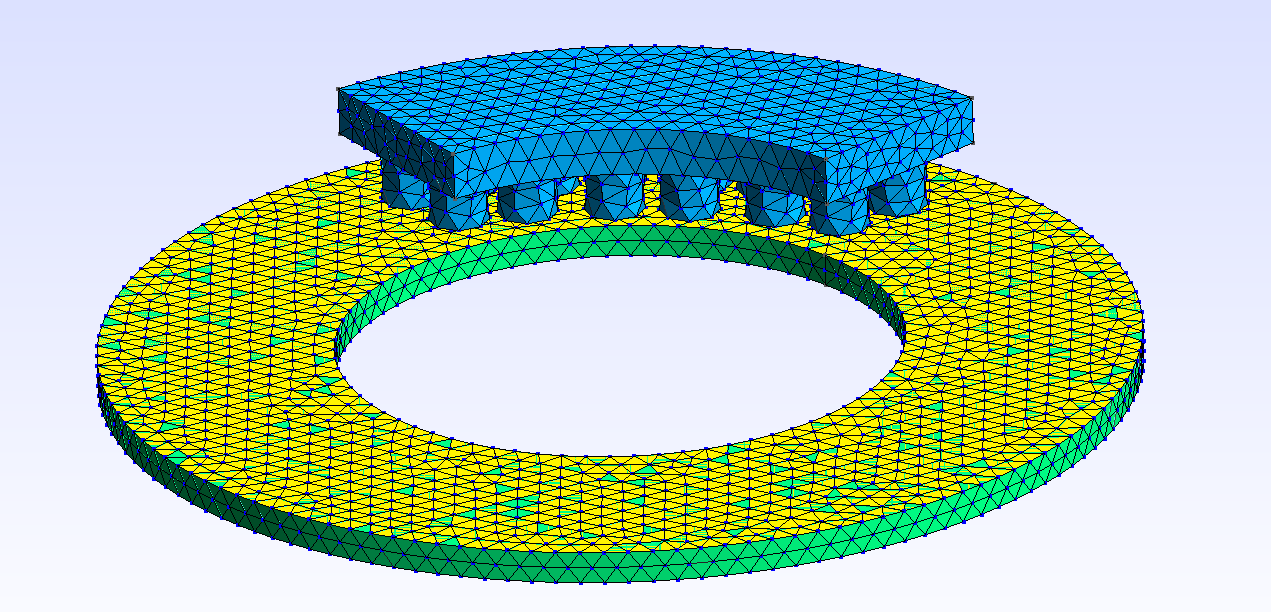
\includegraphics[width=0.9\textwidth]{book/chapters/zhang/graphics/3d surface.png}
    \caption{Computation domain of brake pad and disc, the mesh is much coarser than 1 million case. Friction heat or the Neumann boundary condition is only applied to friction contact areas.}
    \label{fig:coarse mesh}
\end{figure}


\subsection*{Experiment}

The test rig mainly consists of a DC motor, flywheels, brake pad and brake disc, as shown in Figure \ref{fig:test rig}. The maximum motor power is 450 kW, and the maximum motor torque is 4000 Nm. The brake pressure at the reservoir ranges from 0-10 Bar. 
There are in total 6 thermocouples to measure the temperature of the brake disc, which are located under the contact surface. A symmetric model is used in the simulation to save computational effort. The brake lag is the time it takes for the brake pressure to increase from 0\% to 95\% of the target pressure. In the test, the brake lag is 4±0.2 s, which follows the UIC 541-3 standard. Table \ref{tab: operational parameters} shows the operational parameters.

\begin{figure}[h]
    \centering
    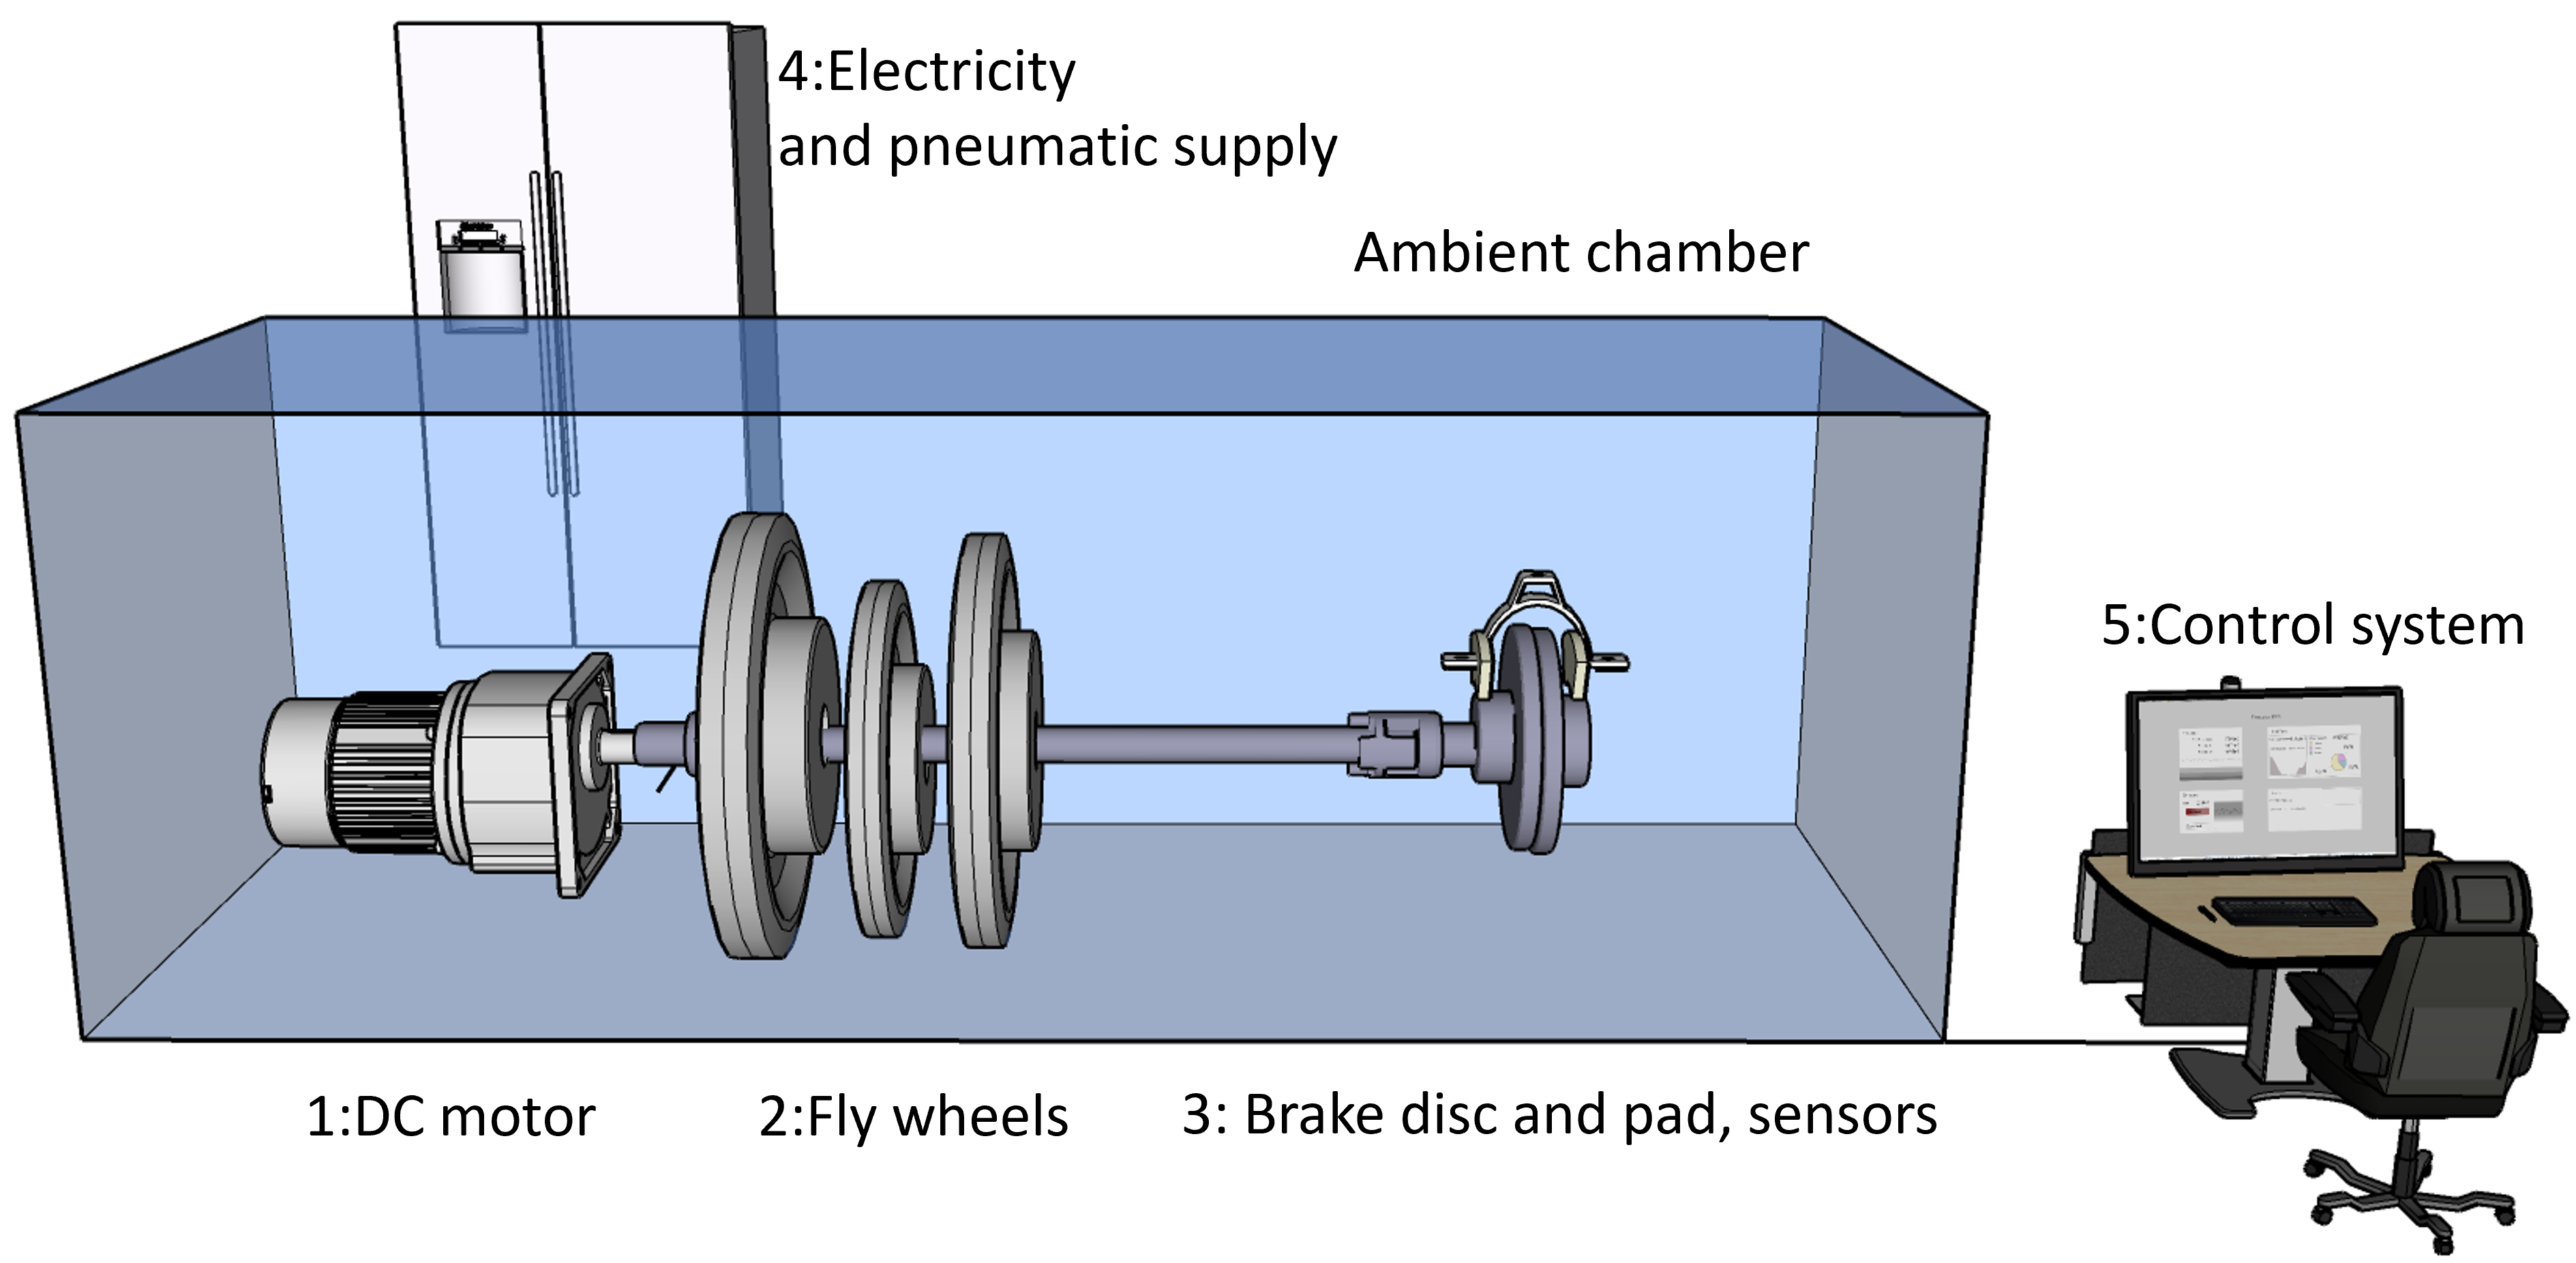
\includegraphics[width=0.85\textwidth]{book/chapters/zhang/graphics/test_rig.png}
    \caption{Full scale railway brake test rig}
    \label{fig:test rig}
\end{figure}

\begin{table}[h]
    \centering
    \begin{tabular}{llll} % 'l' for left-aligned, 'c' for centered
        \toprule
        \textbf{property} & \textbf{quantity} & \textbf{property} & \textbf{quantity}\\ % Header row
        \midrule
        initial velocity (km/h)             & 160       &braking time(s)          & 49 \\
        contact pressure (MPa)              & 0.274      &coefficient of friction  & 0.376 \\
        heat transfer coefficient( W/(m·k)) & 30-125    &heat distributor factor  & 0.88 \\
        brake lag (s)                       & 4         &initial temperature ($^\circ\text{C}$) & 50\\
       
        \bottomrule
    \end{tabular}
    \caption{Brake test parameters}
    \label{tab: operational parameters}
\end{table}

\begin{figure}[h]
    \centering
    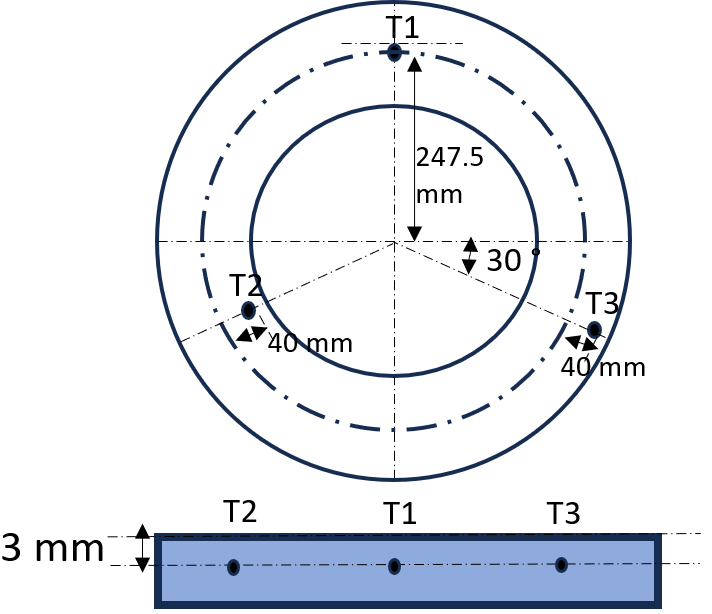
\includegraphics[width=0.45\textwidth]{book/chapters/zhang/graphics/thermo_couples.png}
    \caption{Location of three thermocouples}
    \label{fig:thermocouples}
\end{figure}


\section*{Results and discussion}

\subsection*{Validation}
The first step is mesh sensitivity and time step analysis, where we aim to show that the simulation results converge with finer mesh sizes and smaller time steps. Since no exact solution exist, the average temperature of point T1, as shown in Figure \ref{fig:thermocouples} is used as the convergence parameter.
\begin{figure}
    \centering
    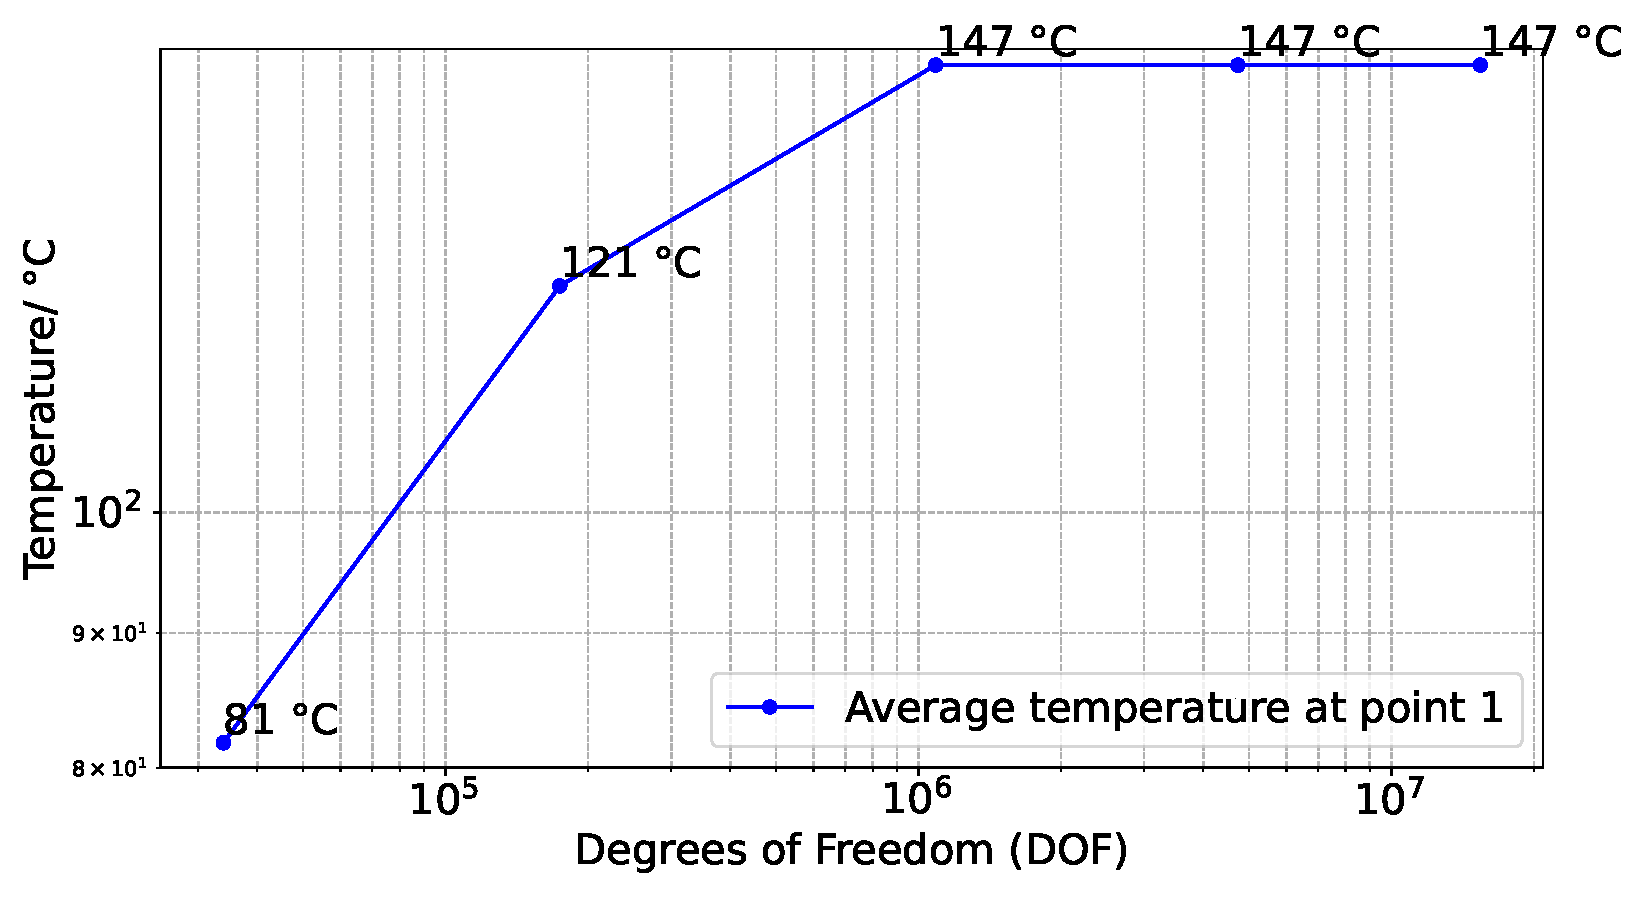
\includegraphics[width=0.8\linewidth]{book/chapters/zhang/graphics/ave_T_vs_dof.pdf}
    \caption{Convergence test, average temperatures of point T1, compared with degrees of freedom (DOFs)}
    \label{fig:error_mesh}
\end{figure}

 As shown in Figure \ref{fig:error_mesh}, the average temperature of point T1 increases with more degrees of freedom until 1 million degrees of freedom (DOFs). Above 1 million, the temperature remains constant.  The above results show that DOFs above 1 million are enough to capture the characteristics of the system. 
\begin{figure}[h]
    \centering
  
    \includegraphics[width=0.8\textwidth]{book/chapters/zhang/graphics/T_ave_vs_dt.pdf}
    \caption{Convergence test, average temperatures of point T1 with time step}
    \label{fig:error_time}
\end{figure}


Figure \ref{fig:error_time} is a comparison of the average temperature of point 1 and times steps. When \(dt\) is above 1 s, the temperature has a large variance. The best value of \(dt\) is 0.16 s (point of 148$^{\circ}\text{C}$ ), which is a balance time step between accuracy and computational time.

\begin{figure}[h]
    \centering
    \includegraphics[width=0.8\textwidth]{book/chapters/zhang/graphics/T_sim_exe.pdf}
    \caption{Comparison between simulation time and experimental results}
    \label{fig:experiment}
\end{figure}

Except for mesh and time sensitivities analysis, the simulation results should validated against the experiment. As shown in Figure \ref{fig:experiment}. The general trend of case 1.2 million elements(4.7 million DOFs) and measurement data are the same, so we think the simulation accuracy is acceptable. However, there is still a large space to improve the accuracy. Such as introducing nonlinear material properties. These parameters, such as thermal conductivity, heat capacity, and coefficient of friction are all not constant or linear with temperature, velocity, and pressure. Getting the exact material characteristics is difficult. So better numerical results can benefit from the research of tribology and material engineering. The more detailed experiment parameters, like the loading pressure, would also significantly improve the numerical results since the experiment tests also contain large variances.



\subsection*{Average and maximum temperatures}

This section presents the temperatures of brake discs with different contact areas. The average and the maximum temperatures are presented.
The total contact surface is 200 cm$^2$. The brake pressures from the back of the brake pads are the same, 0.274 MPa, while the different contact areas will affect the contact pressure between the brake pads and discs. 20\%, 50\% and 100\% contact areas are compared. The 20\% contact areas represent the research from Eriksson \cite{eriksson_nature_2002}, and the 100\% contact areas represent most FEM or analytical solutions.

\begin{figure}[h]
    \centering
    \includegraphics[width=0.8\textwidth]{book/chapters/zhang/graphics/T_ave_dc.pdf}
    \caption{Average temperatures with different contact areas}
    \label{fig:T_ave}
\end{figure}

As shown in Figure \ref{fig:T_ave} is the average temperature for these three cases. The maximum temperature difference is 20 $^{\circ}\text{C}$ between 20\% and 100\% contact areas. The maximum relative difference is 16.6\%. The average temperature is not sensitive to different contact areas since the total heat input is the same, while only heat dissipation is slightly different because the temperature distribution of the brake discs is uneven. Uneven temperature distribution can be proven through the comparison of the maximum temperatures.

\begin{figure}[h]
    \centering
    \includegraphics[width=0.8\textwidth]{book/chapters/zhang/graphics/T_max_dc.pdf}
    \caption{The maximum temperatures with different contact areas}
    \label{fig:T_max}
\end{figure}

Figure \ref{fig:T_max} shows the maximum temperature of the brake discs. The maximum temperature difference is more than 300 $^{\circ}\text{C}$, and the relative difference can reach 160\%. Small contact areas induce higher local temperatures since contact pressure is significantly increased and all friction heat is loaded on limited surfaces.

More advanced research can be conducted based on this FEM model, including sensitivity analysis of railway brake disc temperature development. In the future, the following need to be considered to build a more realistic model to investigate different brake designs:

\begin{enumerate}
\item Coupling elastic equations to get deformation details of the brake pads.
\item Considering more nonlinear parameters, like a variable coefficient of friction, and temperature-dependent material properties.
\end{enumerate}


\section*{Conclusion}
This study investigates the influence of contact area on the temperature of railway brake discs. A FEM model in FEniCSx is built and validated. The following conclusions can be drawn:
\begin{enumerate}
\item The contact area does not influence average temperature significantly while a small contact area induces a higher maximum temperature.
\item FEM based research on thermal analysis of brake systems should model real contact areas between brake pads and discs to get an accurate temperature distribution.
\end{enumerate}


\begin{acknowledgement}
This work is sponsored by the KTH Railway Group, China Scholarship Council and CRRC ZELC. Thanks to the experimental support of Fei Gao, Junying Yang at Dalian Jiaotong University. The help of Jørgen S. Dokken from the FEniCSx community and Jing Gong from Kungliga Tekniska Högskolans PDC support are especially acknowledged. Thanks to the National Academic Infrastructure for Supercomputing in Sweden for providing computer resources.        
\end{acknowledgement}

\bibliographystyle{spbasic}
% Write the full path of your bibfile relative to book.tex

\bibliography{chapters/zhang/bibliography.bib}



% Write the full path to the location of the graphics relative to book.tex
\graphicspath{{chapters/zhang/graphics/}}


\title{Thermal analysis of brake discs in rail vehicles}
\titlerunning{Thermal analysis}

\author{Yanjun Zhang, Sebastian Stichel and William Liu}
\authorrunning{Yanjun et al.}

\institute{Yanjun Zhang \email{yanjunzh@kth.se} \at KTH Royal Institute of Technology}

\maketitle

\abstract{}
Railway brake discs convert the kinetic energy of rail vehicles to thermal energy to achieve braking. This thermal energy deteriorates braking performance, therefore, it is necessary to conduct thermal analyses of brake discs. In this work, we build a FEM (finite element method) model in FEniCSx to investigate the influence of contact areas between brake pads and discs on the temperature of brake discs. The weak form of the nonlinear heat transfer equation has been derived, which accounts for conduction, convection and radiation. Multiple Neumann boundary conditions are applied. Simulation results are validated with experimental results. With this efficient FEM model, more advanced research related to railway brake discs can be conducted, such as investigating the effect of wear and thermal expansion, or designing a new geometry of the brake pads and discs.

\section*{Introduction}
Rail vehicles are developed towards higher speed and higher axle load, requiring robust mechanical brake systems for running safety. As shown in figure \ref{fig:disc_block}, one of the most important mechanical brake systems is the disc brake, which converts the kinetic energy of the rail vehicle into heat. A high brake disc temperature reduces the coefficient of friction between the brake discs and the brake pads \cite{Saffar2010}, and causes high thermal stress, which, in turn, induces thermal cracks on the brake discs. To avoid these negative impacts, it is necessary to study the temperature distribution of brake discs. Experimental investigation is relatively complex and can not obtain some parameters, while numerical study is an effective way to address this issue.

\begin{figure}[h]
    \centering
    \includegraphics[width=0.65\textwidth]{book/chapters/zhang/graphics/disc_block_brakes.png}
    \caption{Block and disc brakes for rail vehicles}
    \label{fig:disc_block}
\end{figure}

Most thermal analyses of brake discs assume full contact between the brake pads and discs. From tribology studies, the real contact area is around 20\% of the whole brake pad friction surface \cite{eriksson_nature_2002}. Because of thermal expansion and wear of the brake pads, the contact area between the brake pads and discs is always changing. It is difficult to predict the true contact area. However, assuming fixed contact areas, the effect on the temperatures of brake discs can be investigated. This research aims to address the effects of different contact areas on the temperature of the brake discs.



\section*{Methods}

\subsection*{Modelling}
Heat generation and dissipation are two main parts of conducting thermal analysis of railway brake discs. Heat flux is based on friction
\begin{equation}
    q_d = \xi F_f V = \xi P A_d \mu V, 
    \label{heat flux}
\end{equation}

where \( q_d \) is the heat flux in the brake discs (W/m$^2$), \( \xi \) is the heat partition coefficient, \( F_f \) is the friction force (N), \( V \) is the velocity (m/s), \( P \) is the local contact pressure between the brake pads and discs (Pa), \( A_d \) is the friction contact area of the brake pads (m$^2$), and \( \mu \) is the coefficient of friction. Equation \ref{heat flux} is the Neumann boundary condition of Equation \ref{heat equation}, which is the overall heat transfer equation.

The heat flux distribution between the brake pads and discs is vital since it depends on how much heat flows to brake discs, which affects the temperatures and stresses. This coefficient is highly non-linear, affected by material, temperature, and pressure. In this research, this coefficient is simplified to a constant number. The distribution factor is described by \cite{rudolf_limpert_brake_1999}
\begin{equation}
    \xi = \frac{q_p}{q_d + q_p},
\end{equation}
where \( q_p \) is the heat flux in the brake pads (W/m$^2$), and \( q_d \) is the heat flux in the brake discs (W/m$^2$). 

The next step is to build a FEM model of the brake disc. FEM is a method to solve partial differential equations. This method includes the discrete domain, uses an appropriate basis, and rewrites algebraic equations. The heat equation is 
\begin{equation}
    \rho c \frac{\partial T}{\partial t} + \nabla \cdot (- k \nabla T) = f,
    \label{heat equation}
\end{equation}
where \( \rho \) is density, \( c \) is thermal capacity, \( T \) is temperature, \( t \) is time, \( k \) is the overall heat transfer coefficient, and \( f \) is the inner heat source. The time derivative on the right-hand side can be approximated by a difference quotient. Here we use the Euler backward method for consideration of numerical stability. After that, all items are multiplied by a test function \( v \) and integrated by parts. Then according to the divergence theorem, the bilinear form \( a(T,v) \) and linear form \( L(v) \) are

\begin{equation}
    a(T,v) = \frac{\rho c}{\Delta t} \int_\Omega T v dx + \int_\Omega k \nabla T \cdot \nabla v dx + \int_{\partial \Omega} h T v ds + \int_{\partial \Omega} \epsilon \sigma T^4 v ds,
\end{equation}

\begin{equation}
    L_{n+1}(v) = \int_\Omega f^{n+1} v dx 
    + \frac{\rho c}{\Delta t} \int_\Omega  T^{n} v dx 
    -  \int_{\partial \Omega} q v ds
    +  \int_{\partial \Omega} h T_a v ds 
    + \int_{\partial \Omega} \epsilon \sigma T_a^4 v ds,
\end{equation}
where \( \Omega \) is the computation domain, \( \partial \Omega \) is the boundary, \( dx \) is the differential element for integration over the domain, and \( ds \) is the differential element for integration over the boundary, \( h \) is the heat convection coefficient,  \(\Delta t\)\ is the time step, \(n\) is an integer counting time levels. The thermal radiation equation is based on Stefan-Boltzmann Law, where \( \epsilon \) is the emissivity, \( \sigma \) is Stefan-Boltzmann constant, \(T\) is the temperature and \(T^4\) is the temperature to the power of four, \( T_a \) is ambient temperature. For more detailed derivation, please see  \href{https://github.com/Yanjun96/fenicsx/blob/main/derivation_of_heat_transfer.pdf}{derivation of weak form for heat transfer equation}.

The above equation is only for heat transfer, as for brake pad deformation, one needs to solve the elastic equation and here we haven't included here. The main contribution of the elastic deformation calculation is a more accurate contact area between the brake pads and the discs. In this study, we assume that the contact area is known a priori since this research focuses on comparing the influence of different contact areas. The above equations are solved in the FEniCSx platform \cite{baratta_dolfinx_2023,scroggs_construction_2022,alnaes_unified_2014}. All the codes for this paper are in \cite{zhang_thermal_2025}.

The computation domain or mesh is shown in Figure \ref{fig:coarse mesh}. This is a much coarser mesh than the one with 1 million elements used later, with around 43,000 elements. The element type is tetrahedron since when we compared it with hexahedral elements, we found with more tetrahedron elements, the simulation can get the same accuracy with hexahedral elements while tetrahedron has less computation time. Only the brake disc and pad are computation domains. The friction heat, or the Neumann boundary condition is applied on the contact surface, more specifically, only the rubbing elements of the brake pad areas. The rubbing elements are the column structure of the brake pad. Other boundaries include radiation and convection heat transfer, which are also the Neumann boundary conditions without the heat flux input. In each time step, the boundary conditions are redefined since the rotation will change the contact area. In reality, the brake pad should keep still while the brake disc rotates. Here we assumed only the heat flux input areas are rotating: these are the friction heat input areas.

\begin{figure}[h]
    \centering
    \includegraphics[width=0.9\textwidth]{book/chapters/zhang/graphics/3d surface.png}
    \caption{Computation domain of brake pad and disc, the mesh is much coarser than 1 million case. Friction heat or the Neumann boundary condition is only applied to friction contact areas.}
    \label{fig:coarse mesh}
\end{figure}


\subsection*{Experiment}

The test rig mainly consists of a DC motor, flywheels, brake pad and brake disc, as shown in Figure \ref{fig:test rig}. The maximum motor power is 450 kW, and the maximum motor torque is 4000 Nm. The brake pressure at the reservoir ranges from 0-10 Bar. 
There are in total 6 thermocouples to measure the temperature of the brake disc, which are located under the contact surface. A symmetric model is used in the simulation to save computational effort. The brake lag is the time it takes for the brake pressure to increase from 0\% to 95\% of the target pressure. In the test, the brake lag is 4±0.2 s, which follows the UIC 541-3 standard. Table \ref{tab: operational parameters} shows the operational parameters.

\begin{figure}[h]
    \centering
    \includegraphics[width=0.85\textwidth]{book/chapters/zhang/graphics/test_rig.png}
    \caption{Full scale railway brake test rig}
    \label{fig:test rig}
\end{figure}

\begin{table}[h]
    \centering
    \begin{tabular}{llll} % 'l' for left-aligned, 'c' for centered
        \toprule
        \textbf{property} & \textbf{quantity} & \textbf{property} & \textbf{quantity}\\ % Header row
        \midrule
        initial velocity (km/h)             & 160       &braking time(s)          & 49 \\
        contact pressure (MPa)              & 0.274      &coefficient of friction  & 0.376 \\
        heat transfer coefficient( W/(m·k)) & 30-125    &heat distributor factor  & 0.88 \\
        brake lag (s)                       & 4         &initial temperature ($^\circ\text{C}$) & 50\\
       
        \bottomrule
    \end{tabular}
    \caption{Brake test parameters}
    \label{tab: operational parameters}
\end{table}

\begin{figure}[h]
    \centering
    \includegraphics[width=0.45\textwidth]{book/chapters/zhang/graphics/thermo_couples.png}
    \caption{Location of three thermocouples}
    \label{fig:thermocouples}
\end{figure}


\section*{Results and discussion}

\subsection*{Validation}
The first step is mesh sensitivity and time step analysis, where we aim to show that the simulation results converge with finer mesh sizes and smaller time steps. Since no exact solution exist, the average temperature of point T1, as shown in Figure \ref{fig:thermocouples} is used as the convergence parameter.
\begin{figure}
    \centering
    \includegraphics[width=0.8\linewidth]{book/chapters/zhang/graphics/ave_T_vs_dof.pdf}
    \caption{Convergence test, average temperatures of point T1, compared with degrees of freedom (DOFs)}
    \label{fig:error_mesh}
\end{figure}

 As shown in Figure \ref{fig:error_mesh}, the average temperature of point T1 increases with more degrees of freedom until 1 million degrees of freedom (DOFs). Above 1 million, the temperature remains constant.  The above results show that DOFs above 1 million are enough to capture the characteristics of the system. 
\begin{figure}[h]
    \centering
  
    \includegraphics[width=0.8\textwidth]{book/chapters/zhang/graphics/T_ave_vs_dt.pdf}
    \caption{Convergence test, average temperatures of point T1 with time step}
    \label{fig:error_time}
\end{figure}


Figure \ref{fig:error_time} is a comparison of the average temperature of point 1 and times steps. When \(dt\) is above 1 s, the temperature has a large variance. The best value of \(dt\) is 0.16 s (point of 148$^{\circ}\text{C}$ ), which is a balance time step between accuracy and computational time.

\begin{figure}[h]
    \centering
    \includegraphics[width=0.8\textwidth]{book/chapters/zhang/graphics/T_sim_exe.pdf}
    \caption{Comparison between simulation time and experimental results}
    \label{fig:experiment}
\end{figure}

Except for mesh and time sensitivities analysis, the simulation results should validated against the experiment. As shown in Figure \ref{fig:experiment}. The general trend of case 1.2 million elements(4.7 million DOFs) and measurement data are the same, so we think the simulation accuracy is acceptable. However, there is still a large space to improve the accuracy. Such as introducing nonlinear material properties. These parameters, such as thermal conductivity, heat capacity, and coefficient of friction are all not constant or linear with temperature, velocity, and pressure. Getting the exact material characteristics is difficult. So better numerical results can benefit from the research of tribology and material engineering. The more detailed experiment parameters, like the loading pressure, would also significantly improve the numerical results since the experiment tests also contain large variances.



\subsection*{Average and maximum temperatures}

This section presents the temperatures of brake discs with different contact areas. The average and the maximum temperatures are presented.
The total contact surface is 200 cm$^2$. The brake pressures from the back of the brake pads are the same, 0.274 MPa, while the different contact areas will affect the contact pressure between the brake pads and discs. 20\%, 50\% and 100\% contact areas are compared. The 20\% contact areas represent the research from Eriksson \cite{eriksson_nature_2002}, and the 100\% contact areas represent most FEM or analytical solutions.

\begin{figure}[h]
    \centering
    \includegraphics[width=0.8\textwidth]{book/chapters/zhang/graphics/T_ave_dc.pdf}
    \caption{Average temperatures with different contact areas}
    \label{fig:T_ave}
\end{figure}

As shown in Figure \ref{fig:T_ave} is the average temperature for these three cases. The maximum temperature difference is 20 $^{\circ}\text{C}$ between 20\% and 100\% contact areas. The maximum relative difference is 16.6\%. The average temperature is not sensitive to different contact areas since the total heat input is the same, while only heat dissipation is slightly different because the temperature distribution of the brake discs is uneven. Uneven temperature distribution can be proven through the comparison of the maximum temperatures.

\begin{figure}[h]
    \centering
    \includegraphics[width=0.8\textwidth]{book/chapters/zhang/graphics/T_max_dc.pdf}
    \caption{The maximum temperatures with different contact areas}
    \label{fig:T_max}
\end{figure}

Figure \ref{fig:T_max} shows the maximum temperature of the brake discs. The maximum temperature difference is more than 300 $^{\circ}\text{C}$, and the relative difference can reach 160\%. Small contact areas induce higher local temperatures since contact pressure is significantly increased and all friction heat is loaded on limited surfaces.

More advanced research can be conducted based on this FEM model, including sensitivity analysis of railway brake disc temperature development. In the future, the following need to be considered to build a more realistic model to investigate different brake designs:

\begin{enumerate}
\item Coupling elastic equations to get deformation details of the brake pads.
\item Considering more nonlinear parameters, like a variable coefficient of friction, and temperature-dependent material properties.
\end{enumerate}


\section*{Conclusion}
This study investigates the influence of contact area on the temperature of railway brake discs. A FEM model in FEniCSx is built and validated. The following conclusions can be drawn:
\begin{enumerate}
\item The contact area does not influence average temperature significantly while a small contact area induces a higher maximum temperature.
\item FEM based research on thermal analysis of brake systems should model real contact areas between brake pads and discs to get an accurate temperature distribution.
\end{enumerate}


\begin{acknowledgement}
This work is sponsored by the KTH Railway Group, China Scholarship Council and CRRC ZELC. Thanks to the experimental support of Fei Gao, Junying Yang at Dalian Jiaotong University. The help of Jørgen S. Dokken from the FEniCSx community and Jing Gong from Kungliga Tekniska Högskolans PDC support are especially acknowledged. Thanks to the National Academic Infrastructure for Supercomputing in Sweden for providing computer resources.        
\end{acknowledgement}

\bibliographystyle{spbasic}
% Write the full path of your bibfile relative to book.tex

\bibliography{chapters/zhang/bibliography.bib}



% Write the full path to the location of the graphics relative to book.tex
\graphicspath{{chapters/zhang/graphics/}}


\title{Thermal analysis of brake discs in rail vehicles}
\titlerunning{Thermal analysis}

\author{Yanjun Zhang, Sebastian Stichel and William Liu}
\authorrunning{Yanjun et al.}

\institute{Yanjun Zhang \email{yanjunzh@kth.se} \at KTH Royal Institute of Technology}

\maketitle

\abstract{}
Railway brake discs convert the kinetic energy of rail vehicles to thermal energy to achieve braking. This thermal energy deteriorates braking performance, therefore, it is necessary to conduct thermal analyses of brake discs. In this work, we build a FEM (finite element method) model in FEniCSx to investigate the influence of contact areas between brake pads and discs on the temperature of brake discs. The weak form of the nonlinear heat transfer equation has been derived, which accounts for conduction, convection and radiation. Multiple Neumann boundary conditions are applied. Simulation results are validated with experimental results. With this efficient FEM model, more advanced research related to railway brake discs can be conducted, such as investigating the effect of wear and thermal expansion, or designing a new geometry of the brake pads and discs.

\section*{Introduction}
Rail vehicles are developed towards higher speed and higher axle load, requiring robust mechanical brake systems for running safety. As shown in figure \ref{fig:disc_block}, one of the most important mechanical brake systems is the disc brake, which converts the kinetic energy of the rail vehicle into heat. A high brake disc temperature reduces the coefficient of friction between the brake discs and the brake pads \cite{Saffar2010}, and causes high thermal stress, which, in turn, induces thermal cracks on the brake discs. To avoid these negative impacts, it is necessary to study the temperature distribution of brake discs. Experimental investigation is relatively complex and can not obtain some parameters, while numerical study is an effective way to address this issue.

\begin{figure}[h]
    \centering
    \includegraphics[width=0.65\textwidth]{book/chapters/zhang/graphics/disc_block_brakes.png}
    \caption{Block and disc brakes for rail vehicles}
    \label{fig:disc_block}
\end{figure}

Most thermal analyses of brake discs assume full contact between the brake pads and discs. From tribology studies, the real contact area is around 20\% of the whole brake pad friction surface \cite{eriksson_nature_2002}. Because of thermal expansion and wear of the brake pads, the contact area between the brake pads and discs is always changing. It is difficult to predict the true contact area. However, assuming fixed contact areas, the effect on the temperatures of brake discs can be investigated. This research aims to address the effects of different contact areas on the temperature of the brake discs.



\section*{Methods}

\subsection*{Modelling}
Heat generation and dissipation are two main parts of conducting thermal analysis of railway brake discs. Heat flux is based on friction
\begin{equation}
    q_d = \xi F_f V = \xi P A_d \mu V, 
    \label{heat flux}
\end{equation}

where \( q_d \) is the heat flux in the brake discs (W/m$^2$), \( \xi \) is the heat partition coefficient, \( F_f \) is the friction force (N), \( V \) is the velocity (m/s), \( P \) is the local contact pressure between the brake pads and discs (Pa), \( A_d \) is the friction contact area of the brake pads (m$^2$), and \( \mu \) is the coefficient of friction. Equation \ref{heat flux} is the Neumann boundary condition of Equation \ref{heat equation}, which is the overall heat transfer equation.

The heat flux distribution between the brake pads and discs is vital since it depends on how much heat flows to brake discs, which affects the temperatures and stresses. This coefficient is highly non-linear, affected by material, temperature, and pressure. In this research, this coefficient is simplified to a constant number. The distribution factor is described by \cite{rudolf_limpert_brake_1999}
\begin{equation}
    \xi = \frac{q_p}{q_d + q_p},
\end{equation}
where \( q_p \) is the heat flux in the brake pads (W/m$^2$), and \( q_d \) is the heat flux in the brake discs (W/m$^2$). 

The next step is to build a FEM model of the brake disc. FEM is a method to solve partial differential equations. This method includes the discrete domain, uses an appropriate basis, and rewrites algebraic equations. The heat equation is 
\begin{equation}
    \rho c \frac{\partial T}{\partial t} + \nabla \cdot (- k \nabla T) = f,
    \label{heat equation}
\end{equation}
where \( \rho \) is density, \( c \) is thermal capacity, \( T \) is temperature, \( t \) is time, \( k \) is the overall heat transfer coefficient, and \( f \) is the inner heat source. The time derivative on the right-hand side can be approximated by a difference quotient. Here we use the Euler backward method for consideration of numerical stability. After that, all items are multiplied by a test function \( v \) and integrated by parts. Then according to the divergence theorem, the bilinear form \( a(T,v) \) and linear form \( L(v) \) are

\begin{equation}
    a(T,v) = \frac{\rho c}{\Delta t} \int_\Omega T v dx + \int_\Omega k \nabla T \cdot \nabla v dx + \int_{\partial \Omega} h T v ds + \int_{\partial \Omega} \epsilon \sigma T^4 v ds,
\end{equation}

\begin{equation}
    L_{n+1}(v) = \int_\Omega f^{n+1} v dx 
    + \frac{\rho c}{\Delta t} \int_\Omega  T^{n} v dx 
    -  \int_{\partial \Omega} q v ds
    +  \int_{\partial \Omega} h T_a v ds 
    + \int_{\partial \Omega} \epsilon \sigma T_a^4 v ds,
\end{equation}
where \( \Omega \) is the computation domain, \( \partial \Omega \) is the boundary, \( dx \) is the differential element for integration over the domain, and \( ds \) is the differential element for integration over the boundary, \( h \) is the heat convection coefficient,  \(\Delta t\)\ is the time step, \(n\) is an integer counting time levels. The thermal radiation equation is based on Stefan-Boltzmann Law, where \( \epsilon \) is the emissivity, \( \sigma \) is Stefan-Boltzmann constant, \(T\) is the temperature and \(T^4\) is the temperature to the power of four, \( T_a \) is ambient temperature. For more detailed derivation, please see  \href{https://github.com/Yanjun96/fenicsx/blob/main/derivation_of_heat_transfer.pdf}{derivation of weak form for heat transfer equation}.

The above equation is only for heat transfer, as for brake pad deformation, one needs to solve the elastic equation and here we haven't included here. The main contribution of the elastic deformation calculation is a more accurate contact area between the brake pads and the discs. In this study, we assume that the contact area is known a priori since this research focuses on comparing the influence of different contact areas. The above equations are solved in the FEniCSx platform \cite{baratta_dolfinx_2023,scroggs_construction_2022,alnaes_unified_2014}. All the codes for this paper are in \cite{zhang_thermal_2025}.

The computation domain or mesh is shown in Figure \ref{fig:coarse mesh}. This is a much coarser mesh than the one with 1 million elements used later, with around 43,000 elements. The element type is tetrahedron since when we compared it with hexahedral elements, we found with more tetrahedron elements, the simulation can get the same accuracy with hexahedral elements while tetrahedron has less computation time. Only the brake disc and pad are computation domains. The friction heat, or the Neumann boundary condition is applied on the contact surface, more specifically, only the rubbing elements of the brake pad areas. The rubbing elements are the column structure of the brake pad. Other boundaries include radiation and convection heat transfer, which are also the Neumann boundary conditions without the heat flux input. In each time step, the boundary conditions are redefined since the rotation will change the contact area. In reality, the brake pad should keep still while the brake disc rotates. Here we assumed only the heat flux input areas are rotating: these are the friction heat input areas.

\begin{figure}[h]
    \centering
    \includegraphics[width=0.9\textwidth]{book/chapters/zhang/graphics/3d surface.png}
    \caption{Computation domain of brake pad and disc, the mesh is much coarser than 1 million case. Friction heat or the Neumann boundary condition is only applied to friction contact areas.}
    \label{fig:coarse mesh}
\end{figure}


\subsection*{Experiment}

The test rig mainly consists of a DC motor, flywheels, brake pad and brake disc, as shown in Figure \ref{fig:test rig}. The maximum motor power is 450 kW, and the maximum motor torque is 4000 Nm. The brake pressure at the reservoir ranges from 0-10 Bar. 
There are in total 6 thermocouples to measure the temperature of the brake disc, which are located under the contact surface. A symmetric model is used in the simulation to save computational effort. The brake lag is the time it takes for the brake pressure to increase from 0\% to 95\% of the target pressure. In the test, the brake lag is 4±0.2 s, which follows the UIC 541-3 standard. Table \ref{tab: operational parameters} shows the operational parameters.

\begin{figure}[h]
    \centering
    \includegraphics[width=0.85\textwidth]{book/chapters/zhang/graphics/test_rig.png}
    \caption{Full scale railway brake test rig}
    \label{fig:test rig}
\end{figure}

\begin{table}[h]
    \centering
    \begin{tabular}{llll} % 'l' for left-aligned, 'c' for centered
        \toprule
        \textbf{property} & \textbf{quantity} & \textbf{property} & \textbf{quantity}\\ % Header row
        \midrule
        initial velocity (km/h)             & 160       &braking time(s)          & 49 \\
        contact pressure (MPa)              & 0.274      &coefficient of friction  & 0.376 \\
        heat transfer coefficient( W/(m·k)) & 30-125    &heat distributor factor  & 0.88 \\
        brake lag (s)                       & 4         &initial temperature ($^\circ\text{C}$) & 50\\
       
        \bottomrule
    \end{tabular}
    \caption{Brake test parameters}
    \label{tab: operational parameters}
\end{table}

\begin{figure}[h]
    \centering
    \includegraphics[width=0.45\textwidth]{book/chapters/zhang/graphics/thermo_couples.png}
    \caption{Location of three thermocouples}
    \label{fig:thermocouples}
\end{figure}


\section*{Results and discussion}

\subsection*{Validation}
The first step is mesh sensitivity and time step analysis, where we aim to show that the simulation results converge with finer mesh sizes and smaller time steps. Since no exact solution exist, the average temperature of point T1, as shown in Figure \ref{fig:thermocouples} is used as the convergence parameter.
\begin{figure}
    \centering
    \includegraphics[width=0.8\linewidth]{book/chapters/zhang/graphics/ave_T_vs_dof.pdf}
    \caption{Convergence test, average temperatures of point T1, compared with degrees of freedom (DOFs)}
    \label{fig:error_mesh}
\end{figure}

 As shown in Figure \ref{fig:error_mesh}, the average temperature of point T1 increases with more degrees of freedom until 1 million degrees of freedom (DOFs). Above 1 million, the temperature remains constant.  The above results show that DOFs above 1 million are enough to capture the characteristics of the system. 
\begin{figure}[h]
    \centering
  
    \includegraphics[width=0.8\textwidth]{book/chapters/zhang/graphics/T_ave_vs_dt.pdf}
    \caption{Convergence test, average temperatures of point T1 with time step}
    \label{fig:error_time}
\end{figure}


Figure \ref{fig:error_time} is a comparison of the average temperature of point 1 and times steps. When \(dt\) is above 1 s, the temperature has a large variance. The best value of \(dt\) is 0.16 s (point of 148$^{\circ}\text{C}$ ), which is a balance time step between accuracy and computational time.

\begin{figure}[h]
    \centering
    \includegraphics[width=0.8\textwidth]{book/chapters/zhang/graphics/T_sim_exe.pdf}
    \caption{Comparison between simulation time and experimental results}
    \label{fig:experiment}
\end{figure}

Except for mesh and time sensitivities analysis, the simulation results should validated against the experiment. As shown in Figure \ref{fig:experiment}. The general trend of case 1.2 million elements(4.7 million DOFs) and measurement data are the same, so we think the simulation accuracy is acceptable. However, there is still a large space to improve the accuracy. Such as introducing nonlinear material properties. These parameters, such as thermal conductivity, heat capacity, and coefficient of friction are all not constant or linear with temperature, velocity, and pressure. Getting the exact material characteristics is difficult. So better numerical results can benefit from the research of tribology and material engineering. The more detailed experiment parameters, like the loading pressure, would also significantly improve the numerical results since the experiment tests also contain large variances.



\subsection*{Average and maximum temperatures}

This section presents the temperatures of brake discs with different contact areas. The average and the maximum temperatures are presented.
The total contact surface is 200 cm$^2$. The brake pressures from the back of the brake pads are the same, 0.274 MPa, while the different contact areas will affect the contact pressure between the brake pads and discs. 20\%, 50\% and 100\% contact areas are compared. The 20\% contact areas represent the research from Eriksson \cite{eriksson_nature_2002}, and the 100\% contact areas represent most FEM or analytical solutions.

\begin{figure}[h]
    \centering
    \includegraphics[width=0.8\textwidth]{book/chapters/zhang/graphics/T_ave_dc.pdf}
    \caption{Average temperatures with different contact areas}
    \label{fig:T_ave}
\end{figure}

As shown in Figure \ref{fig:T_ave} is the average temperature for these three cases. The maximum temperature difference is 20 $^{\circ}\text{C}$ between 20\% and 100\% contact areas. The maximum relative difference is 16.6\%. The average temperature is not sensitive to different contact areas since the total heat input is the same, while only heat dissipation is slightly different because the temperature distribution of the brake discs is uneven. Uneven temperature distribution can be proven through the comparison of the maximum temperatures.

\begin{figure}[h]
    \centering
    \includegraphics[width=0.8\textwidth]{book/chapters/zhang/graphics/T_max_dc.pdf}
    \caption{The maximum temperatures with different contact areas}
    \label{fig:T_max}
\end{figure}

Figure \ref{fig:T_max} shows the maximum temperature of the brake discs. The maximum temperature difference is more than 300 $^{\circ}\text{C}$, and the relative difference can reach 160\%. Small contact areas induce higher local temperatures since contact pressure is significantly increased and all friction heat is loaded on limited surfaces.

More advanced research can be conducted based on this FEM model, including sensitivity analysis of railway brake disc temperature development. In the future, the following need to be considered to build a more realistic model to investigate different brake designs:

\begin{enumerate}
\item Coupling elastic equations to get deformation details of the brake pads.
\item Considering more nonlinear parameters, like a variable coefficient of friction, and temperature-dependent material properties.
\end{enumerate}


\section*{Conclusion}
This study investigates the influence of contact area on the temperature of railway brake discs. A FEM model in FEniCSx is built and validated. The following conclusions can be drawn:
\begin{enumerate}
\item The contact area does not influence average temperature significantly while a small contact area induces a higher maximum temperature.
\item FEM based research on thermal analysis of brake systems should model real contact areas between brake pads and discs to get an accurate temperature distribution.
\end{enumerate}


\begin{acknowledgement}
This work is sponsored by the KTH Railway Group, China Scholarship Council and CRRC ZELC. Thanks to the experimental support of Fei Gao, Junying Yang at Dalian Jiaotong University. The help of Jørgen S. Dokken from the FEniCSx community and Jing Gong from Kungliga Tekniska Högskolans PDC support are especially acknowledged. Thanks to the National Academic Infrastructure for Supercomputing in Sweden for providing computer resources.        
\end{acknowledgement}

\bibliographystyle{spbasic}
% Write the full path of your bibfile relative to book.tex

\bibliography{chapters/zhang/bibliography.bib}



% Write the full path to the location of the graphics relative to book.tex
\graphicspath{{chapters/zhang/graphics/}}


\title{Thermal analysis of brake discs in rail vehicles}
\titlerunning{Thermal analysis}

\author{Yanjun Zhang, Sebastian Stichel and William Liu}
\authorrunning{Yanjun et al.}

\institute{Yanjun Zhang \email{yanjunzh@kth.se} \at KTH Royal Institute of Technology}

\maketitle

\abstract{}
Railway brake discs convert the kinetic energy of rail vehicles to thermal energy to achieve braking. This thermal energy deteriorates braking performance, therefore, it is necessary to conduct thermal analyses of brake discs. In this work, we build a FEM (finite element method) model in FEniCSx to investigate the influence of contact areas between brake pads and discs on the temperature of brake discs. The weak form of the nonlinear heat transfer equation has been derived, which accounts for conduction, convection and radiation. Multiple Neumann boundary conditions are applied. Simulation results are validated with experimental results. With this efficient FEM model, more advanced research related to railway brake discs can be conducted, such as investigating the effect of wear and thermal expansion, or designing a new geometry of the brake pads and discs.

\section*{Introduction}
Rail vehicles are developed towards higher speed and higher axle load, requiring robust mechanical brake systems for running safety. As shown in figure \ref{fig:disc_block}, one of the most important mechanical brake systems is the disc brake, which converts the kinetic energy of the rail vehicle into heat. A high brake disc temperature reduces the coefficient of friction between the brake discs and the brake pads \cite{Saffar2010}, and causes high thermal stress, which, in turn, induces thermal cracks on the brake discs. To avoid these negative impacts, it is necessary to study the temperature distribution of brake discs. Experimental investigation is relatively complex and can not obtain some parameters, while numerical study is an effective way to address this issue.

\begin{figure}[h]
    \centering
    \includegraphics[width=0.65\textwidth]{book/chapters/zhang/graphics/disc_block_brakes.png}
    \caption{Block and disc brakes for rail vehicles}
    \label{fig:disc_block}
\end{figure}

Most thermal analyses of brake discs assume full contact between the brake pads and discs. From tribology studies, the real contact area is around 20\% of the whole brake pad friction surface \cite{eriksson_nature_2002}. Because of thermal expansion and wear of the brake pads, the contact area between the brake pads and discs is always changing. It is difficult to predict the true contact area. However, assuming fixed contact areas, the effect on the temperatures of brake discs can be investigated. This research aims to address the effects of different contact areas on the temperature of the brake discs.



\section*{Methods}

\subsection*{Modelling}
Heat generation and dissipation are two main parts of conducting thermal analysis of railway brake discs. Heat flux is based on friction
\begin{equation}
    q_d = \xi F_f V = \xi P A_d \mu V, 
    \label{heat flux}
\end{equation}

where \( q_d \) is the heat flux in the brake discs (W/m$^2$), \( \xi \) is the heat partition coefficient, \( F_f \) is the friction force (N), \( V \) is the velocity (m/s), \( P \) is the local contact pressure between the brake pads and discs (Pa), \( A_d \) is the friction contact area of the brake pads (m$^2$), and \( \mu \) is the coefficient of friction. Equation \ref{heat flux} is the Neumann boundary condition of Equation \ref{heat equation}, which is the overall heat transfer equation.

The heat flux distribution between the brake pads and discs is vital since it depends on how much heat flows to brake discs, which affects the temperatures and stresses. This coefficient is highly non-linear, affected by material, temperature, and pressure. In this research, this coefficient is simplified to a constant number. The distribution factor is described by \cite{rudolf_limpert_brake_1999}
\begin{equation}
    \xi = \frac{q_p}{q_d + q_p},
\end{equation}
where \( q_p \) is the heat flux in the brake pads (W/m$^2$), and \( q_d \) is the heat flux in the brake discs (W/m$^2$). 

The next step is to build a FEM model of the brake disc. FEM is a method to solve partial differential equations. This method includes the discrete domain, uses an appropriate basis, and rewrites algebraic equations. The heat equation is 
\begin{equation}
    \rho c \frac{\partial T}{\partial t} + \nabla \cdot (- k \nabla T) = f,
    \label{heat equation}
\end{equation}
where \( \rho \) is density, \( c \) is thermal capacity, \( T \) is temperature, \( t \) is time, \( k \) is the overall heat transfer coefficient, and \( f \) is the inner heat source. The time derivative on the right-hand side can be approximated by a difference quotient. Here we use the Euler backward method for consideration of numerical stability. After that, all items are multiplied by a test function \( v \) and integrated by parts. Then according to the divergence theorem, the bilinear form \( a(T,v) \) and linear form \( L(v) \) are

\begin{equation}
    a(T,v) = \frac{\rho c}{\Delta t} \int_\Omega T v dx + \int_\Omega k \nabla T \cdot \nabla v dx + \int_{\partial \Omega} h T v ds + \int_{\partial \Omega} \epsilon \sigma T^4 v ds,
\end{equation}

\begin{equation}
    L_{n+1}(v) = \int_\Omega f^{n+1} v dx 
    + \frac{\rho c}{\Delta t} \int_\Omega  T^{n} v dx 
    -  \int_{\partial \Omega} q v ds
    +  \int_{\partial \Omega} h T_a v ds 
    + \int_{\partial \Omega} \epsilon \sigma T_a^4 v ds,
\end{equation}
where \( \Omega \) is the computation domain, \( \partial \Omega \) is the boundary, \( dx \) is the differential element for integration over the domain, and \( ds \) is the differential element for integration over the boundary, \( h \) is the heat convection coefficient,  \(\Delta t\)\ is the time step, \(n\) is an integer counting time levels. The thermal radiation equation is based on Stefan-Boltzmann Law, where \( \epsilon \) is the emissivity, \( \sigma \) is Stefan-Boltzmann constant, \(T\) is the temperature and \(T^4\) is the temperature to the power of four, \( T_a \) is ambient temperature. For more detailed derivation, please see  \href{https://github.com/Yanjun96/fenicsx/blob/main/derivation_of_heat_transfer.pdf}{derivation of weak form for heat transfer equation}.

The above equation is only for heat transfer, as for brake pad deformation, one needs to solve the elastic equation and here we haven't included here. The main contribution of the elastic deformation calculation is a more accurate contact area between the brake pads and the discs. In this study, we assume that the contact area is known a priori since this research focuses on comparing the influence of different contact areas. The above equations are solved in the FEniCSx platform \cite{baratta_dolfinx_2023,scroggs_construction_2022,alnaes_unified_2014}. All the codes for this paper are in \cite{zhang_thermal_2025}.

The computation domain or mesh is shown in Figure \ref{fig:coarse mesh}. This is a much coarser mesh than the one with 1 million elements used later, with around 43,000 elements. The element type is tetrahedron since when we compared it with hexahedral elements, we found with more tetrahedron elements, the simulation can get the same accuracy with hexahedral elements while tetrahedron has less computation time. Only the brake disc and pad are computation domains. The friction heat, or the Neumann boundary condition is applied on the contact surface, more specifically, only the rubbing elements of the brake pad areas. The rubbing elements are the column structure of the brake pad. Other boundaries include radiation and convection heat transfer, which are also the Neumann boundary conditions without the heat flux input. In each time step, the boundary conditions are redefined since the rotation will change the contact area. In reality, the brake pad should keep still while the brake disc rotates. Here we assumed only the heat flux input areas are rotating: these are the friction heat input areas.

\begin{figure}[h]
    \centering
    \includegraphics[width=0.9\textwidth]{book/chapters/zhang/graphics/3d surface.png}
    \caption{Computation domain of brake pad and disc, the mesh is much coarser than 1 million case. Friction heat or the Neumann boundary condition is only applied to friction contact areas.}
    \label{fig:coarse mesh}
\end{figure}


\subsection*{Experiment}

The test rig mainly consists of a DC motor, flywheels, brake pad and brake disc, as shown in Figure \ref{fig:test rig}. The maximum motor power is 450 kW, and the maximum motor torque is 4000 Nm. The brake pressure at the reservoir ranges from 0-10 Bar. 
There are in total 6 thermocouples to measure the temperature of the brake disc, which are located under the contact surface. A symmetric model is used in the simulation to save computational effort. The brake lag is the time it takes for the brake pressure to increase from 0\% to 95\% of the target pressure. In the test, the brake lag is 4±0.2 s, which follows the UIC 541-3 standard. Table \ref{tab: operational parameters} shows the operational parameters.

\begin{figure}[h]
    \centering
    \includegraphics[width=0.85\textwidth]{book/chapters/zhang/graphics/test_rig.png}
    \caption{Full scale railway brake test rig}
    \label{fig:test rig}
\end{figure}

\begin{table}[h]
    \centering
    \begin{tabular}{llll} % 'l' for left-aligned, 'c' for centered
        \toprule
        \textbf{property} & \textbf{quantity} & \textbf{property} & \textbf{quantity}\\ % Header row
        \midrule
        initial velocity (km/h)             & 160       &braking time(s)          & 49 \\
        contact pressure (MPa)              & 0.274      &coefficient of friction  & 0.376 \\
        heat transfer coefficient( W/(m·k)) & 30-125    &heat distributor factor  & 0.88 \\
        brake lag (s)                       & 4         &initial temperature ($^\circ\text{C}$) & 50\\
       
        \bottomrule
    \end{tabular}
    \caption{Brake test parameters}
    \label{tab: operational parameters}
\end{table}

\begin{figure}[h]
    \centering
    \includegraphics[width=0.45\textwidth]{book/chapters/zhang/graphics/thermo_couples.png}
    \caption{Location of three thermocouples}
    \label{fig:thermocouples}
\end{figure}


\section*{Results and discussion}

\subsection*{Validation}
The first step is mesh sensitivity and time step analysis, where we aim to show that the simulation results converge with finer mesh sizes and smaller time steps. Since no exact solution exist, the average temperature of point T1, as shown in Figure \ref{fig:thermocouples} is used as the convergence parameter.
\begin{figure}
    \centering
    \includegraphics[width=0.8\linewidth]{book/chapters/zhang/graphics/ave_T_vs_dof.pdf}
    \caption{Convergence test, average temperatures of point T1, compared with degrees of freedom (DOFs)}
    \label{fig:error_mesh}
\end{figure}

 As shown in Figure \ref{fig:error_mesh}, the average temperature of point T1 increases with more degrees of freedom until 1 million degrees of freedom (DOFs). Above 1 million, the temperature remains constant.  The above results show that DOFs above 1 million are enough to capture the characteristics of the system. 
\begin{figure}[h]
    \centering
  
    \includegraphics[width=0.8\textwidth]{book/chapters/zhang/graphics/T_ave_vs_dt.pdf}
    \caption{Convergence test, average temperatures of point T1 with time step}
    \label{fig:error_time}
\end{figure}


Figure \ref{fig:error_time} is a comparison of the average temperature of point 1 and times steps. When \(dt\) is above 1 s, the temperature has a large variance. The best value of \(dt\) is 0.16 s (point of 148$^{\circ}\text{C}$ ), which is a balance time step between accuracy and computational time.

\begin{figure}[h]
    \centering
    \includegraphics[width=0.8\textwidth]{book/chapters/zhang/graphics/T_sim_exe.pdf}
    \caption{Comparison between simulation time and experimental results}
    \label{fig:experiment}
\end{figure}

Except for mesh and time sensitivities analysis, the simulation results should validated against the experiment. As shown in Figure \ref{fig:experiment}. The general trend of case 1.2 million elements(4.7 million DOFs) and measurement data are the same, so we think the simulation accuracy is acceptable. However, there is still a large space to improve the accuracy. Such as introducing nonlinear material properties. These parameters, such as thermal conductivity, heat capacity, and coefficient of friction are all not constant or linear with temperature, velocity, and pressure. Getting the exact material characteristics is difficult. So better numerical results can benefit from the research of tribology and material engineering. The more detailed experiment parameters, like the loading pressure, would also significantly improve the numerical results since the experiment tests also contain large variances.



\subsection*{Average and maximum temperatures}

This section presents the temperatures of brake discs with different contact areas. The average and the maximum temperatures are presented.
The total contact surface is 200 cm$^2$. The brake pressures from the back of the brake pads are the same, 0.274 MPa, while the different contact areas will affect the contact pressure between the brake pads and discs. 20\%, 50\% and 100\% contact areas are compared. The 20\% contact areas represent the research from Eriksson \cite{eriksson_nature_2002}, and the 100\% contact areas represent most FEM or analytical solutions.

\begin{figure}[h]
    \centering
    \includegraphics[width=0.8\textwidth]{book/chapters/zhang/graphics/T_ave_dc.pdf}
    \caption{Average temperatures with different contact areas}
    \label{fig:T_ave}
\end{figure}

As shown in Figure \ref{fig:T_ave} is the average temperature for these three cases. The maximum temperature difference is 20 $^{\circ}\text{C}$ between 20\% and 100\% contact areas. The maximum relative difference is 16.6\%. The average temperature is not sensitive to different contact areas since the total heat input is the same, while only heat dissipation is slightly different because the temperature distribution of the brake discs is uneven. Uneven temperature distribution can be proven through the comparison of the maximum temperatures.

\begin{figure}[h]
    \centering
    \includegraphics[width=0.8\textwidth]{book/chapters/zhang/graphics/T_max_dc.pdf}
    \caption{The maximum temperatures with different contact areas}
    \label{fig:T_max}
\end{figure}

Figure \ref{fig:T_max} shows the maximum temperature of the brake discs. The maximum temperature difference is more than 300 $^{\circ}\text{C}$, and the relative difference can reach 160\%. Small contact areas induce higher local temperatures since contact pressure is significantly increased and all friction heat is loaded on limited surfaces.

More advanced research can be conducted based on this FEM model, including sensitivity analysis of railway brake disc temperature development. In the future, the following need to be considered to build a more realistic model to investigate different brake designs:

\begin{enumerate}
\item Coupling elastic equations to get deformation details of the brake pads.
\item Considering more nonlinear parameters, like a variable coefficient of friction, and temperature-dependent material properties.
\end{enumerate}


\section*{Conclusion}
This study investigates the influence of contact area on the temperature of railway brake discs. A FEM model in FEniCSx is built and validated. The following conclusions can be drawn:
\begin{enumerate}
\item The contact area does not influence average temperature significantly while a small contact area induces a higher maximum temperature.
\item FEM based research on thermal analysis of brake systems should model real contact areas between brake pads and discs to get an accurate temperature distribution.
\end{enumerate}


\begin{acknowledgement}
This work is sponsored by the KTH Railway Group, China Scholarship Council and CRRC ZELC. Thanks to the experimental support of Fei Gao, Junying Yang at Dalian Jiaotong University. The help of Jørgen S. Dokken from the FEniCSx community and Jing Gong from Kungliga Tekniska Högskolans PDC support are especially acknowledged. Thanks to the National Academic Infrastructure for Supercomputing in Sweden for providing computer resources.        
\end{acknowledgement}

\bibliographystyle{spbasic}
% Write the full path of your bibfile relative to book.tex

\bibliography{chapters/zhang/bibliography.bib}




\backmatter%%%%%%%%%%%%%%%%%%%%%%%%%%%%%%%%%%%%%%%%%%%%%%%%%%%%%%%
\appendix
%\include{appendix}
% --- Matrices and vector definitions ---
\renewcommand{\vec}[1]{\bm{\mathrm{#1}}}
\newcommand{\vecGreek}[1]{\bm{#1}}
\newcommand{\mat}[1]{\bm{\mathrm{#1}}}
\newcommand{\matGreek}[1]{\bm{#1}}

% --- The defined symbols ---
\newcommand{\sbReference}{0}
\newcommand{\sbReferenceSolid}{0\solid}
\newcommand{\spPhase}{\phase}
\newcommand{\spPhaseReal}{\phase\mathrm{R}}
\newcommand{\sbPhase}{\phase}
\newcommand{\spDimension}{d}
\newcommand{\sbElemental}{e}
\newcommand{\spFluid}{\fluid}
\newcommand{\spFluidReal}{\fluid\mathrm{R}}
\newcommand{\sbFluid}{\fluid}
\newcommand{\spDiscrete}{h}
\newcommand{\spEqlb}{\mathrm{R}}
\newcommand{\spSolid}{\solid}
\newcommand{\spSolidExtra}{\solid\mathrm{E}}
\newcommand{\spSolidReal}{\solid\mathrm{R}}
\newcommand{\sbSolid}{\solid}
\newcommand{\gdim}{d}
\newcommand{\elmt}{e}
\newcommand{\h}{h}
\newcommand{\eqlb}{\mathrm{R}}
\newcommand{\defCauchyGreenRight}{\mat{C}}
\newcommand{\strainGreenLagrange}{\mat{E}}
\newcommand{\YoungsMod}{\mathrm{E}}
\newcommand{\DefGrad}{\mat{F}}
\newcommand{\stressPKi}{\mat{P}}
\newcommand{\stressPKii}{\mat{S}}
\newcommand{\xRef}{\vec{X}}
\newcommand{\xCur}{\vec{x}}
\newcommand{\CsbS}{\mat{C}_{\solid}}
\newcommand{\EsbS}{\mat{E}_{\solid}}
\newcommand{\YoungsModspS}{\mathrm{E}^{\solid}}
\newcommand{\FsbS}{\mat{F}_{\solid}}
\newcommand{\PispS}{\mat{P}^{\solid}}
\newcommand{\PispSE}{\mat{P}^{\solid\mathrm{E}}}
\newcommand{\PispF}{\mat{P}^{\fluid}}
\newcommand{\PiispS}{\mat{S}^{\solid}}
\newcommand{\PiispSE}{\mat{S}^{\solid\mathrm{E}}}
\newcommand{\PiispF}{\mat{S}^{\fluid}}
\newcommand{\XsbPhase}{\vec{X}_{\phase}}
\newcommand{\XsbS}{\vec{X}_{\solid}}
\newcommand{\XsbF}{\vec{X}_{\fluid}}
\newcommand{\xsbPhase}{\vec{x}_{\phase}}
\newcommand{\xsbS}{\vec{x}_{\solid}}
\newcommand{\xsbF}{\vec{x}_{\fluid}}
\newcommand{\strainGreenLagrangeLin}{\matGreek{\varepsilon}}
\newcommand{\Lamei}{\lambda}
\newcommand{\Lameii}{\mu}
\newcommand{\PoissonsRatio}{\nu}
\newcommand{\stressPKLin}{\matGreek{\sigma}}
\newcommand{\LinEsbS}{\matGreek{\varepsilon}_{\solid}}
\newcommand{\lispS}{\lambda^{\solid}}
\newcommand{\liispS}{\mu^{\solid}}
\newcommand{\nuspS}{\nu^{\solid}}
\newcommand{\LinPKspS}{\matGreek{\sigma}^{\solid}}
\newcommand{\LinPKspSE}{\matGreek{\sigma}^{\solid\mathrm{E}}}
\newcommand{\LinPKspF}{\matGreek{\sigma}^{\fluid}}
\newcommand{\LinPKEqlb}{\matGreek{\sigma}^{\mathrm{R}}}
\newcommand{\LinPKEqlbH}{\matGreek{\sigma}^{\mathrm{R}}_\h}
\newcommand{\Displacement}{\vec{u}}

\printindex

%%%%%%%%%%%%%%%%%%%%%%%%%%%%%%%%%%%%%%%%%%%%%%%%%%%%%%%%%%%%%%%%%%%%%%

\end{document}

